\documentclass[12pt,a4paper]{article}
\usepackage[utf8]{inputenc}
\usepackage[T1]{fontenc}
\usepackage[english]{babel}
\usepackage[english]{isodate}
\usepackage[paper=a4paper]{geometry}
\newgeometry{top=3.5cm,bottom=2.5cm,right=2.5cm,left=2.5cm}
\usepackage{graphicx}
\usepackage{comment}
\usepackage{fancyhdr}
\usepackage{framed}
\usepackage{lastpage}
\usepackage[hidelinks]{hyperref}
\usepackage{tabularx}
\usepackage[table]{xcolor}
\usepackage{enumitem}
\usepackage{mdwlist}
\usepackage{placeins}
\usepackage{amsmath}
\usepackage{xcolor}
\usepackage{listings}
\usepackage{amssymb}
\usepackage{amsthm}
\usepackage{xparse}
\usepackage{float}
\usepackage{chngcntr}

\counterwithin*{equation}{section}
\counterwithin*{equation}{subsection}


\begin{document}

\newcommand{\titolo}{Information Retrieval and Web Search}
\newcommand{\versione}{2.0}

\newcommand{\imageB}[2]{ 
        % 1 = image 
        % 2 = size
	\begin{figure}[h!]
    	\centering
    	\includegraphics[scale = #2]{img/#1} 
	\end{figure}
}

\newcommand{\image}[3]{
        % 1 = image 
        % 2 = size
        % 3 = caption
        \begin{figure}[h!]
    	\centering
    	\includegraphics[scale = #2]{img/#1} 
    	\caption{#3}
	\end{figure}
}

\newcommand{\imageLabel}[4]{ 
        % 1 = image 
        % 2 = size
        % 3 = caption
        % 4 = label
	\begin{figure}[h!]
    	\centering
    	\includegraphics[scale = #2]{img/#1} 
            \label{#4}
    	\caption{#3} 
	\end{figure}
}

\newcommand{\Z}{\mathbb{Z}}

\newcommand{\definition}[2]{
\vspace{3mm} \textbf{Definition (#1).} \textit{#2} \vspace{3mm}
}

\newcommand{\example}[1]{
\vspace{3mm} \textbf{Example.} \textit{#1} \vspace{3mm}
}

\newcommand{\theorem}[1]{
\vspace{3mm} \textbf{Theorem.} \textit{#1} \vspace{1mm}
}

\newcommand{\theoremNum}[2]{
\vspace{3mm} \textbf{Theorem #1.} \textit{#2} \vspace{1mm}
}

\newcommand{\theoremName}[2]{
\vspace{3mm} \textbf{Theorem (#1).} \textit{#2} \vspace{1mm}
}

\newcommand{\theoremBox}[1]{
\vspace{3mm} \begin{tcolorbox} \textbf{Theorem.} \textit{#1} \end{tcolorbox} \vspace{1mm}
}

\newcommand{\theoremNameBox}[2]{
\vspace{3mm} \begin{tcolorbox} \textbf{Theorem (#1).} \textit{#2} \end{tcolorbox} \vspace{1mm}
}

\newcommand{\theoremNumBox}[2]{
\vspace{3mm} \begin{tcolorbox} \textbf{Theorem #1.} \textit{#2} \end{tcolorbox} \vspace{1mm}
}

\newcommand{\lemma}[2]{
\vspace{3mm} \textbf{Lemma #1.} \textit{#2} \vspace{1mm}
}

\newcommand{\lemmaName}[2]{
\vspace{3mm} \textbf{Lemma (#1).} \textit{#2} \vspace{1mm}
}

\newcommand{\claim}[1]{
\vspace{3mm} \textbf{Claim.} \textit{#1} \vspace{1mm}
}

\pagenumbering{Alph}
\begin{titlepage}
	\begin{center}
		
\includegraphics[width=0.6\textwidth]{unive}
		
		\vspace*{1cm}
		\LARGE
		%\textit{Foundations of Machine Learning \\
	%		\center Year: 2022/2023}
		
		\vspace{0.5cm}
		\Huge
		\textbf{\titolo}\\
		
		\line(1,0){280}
		
		\vspace{0.5cm}
		\large
		\textit{Academic Year 2023/2024}
		
		\vfill
		
	\end{center}
	\begin{raggedleft}
		\Large
		%Team: \textbf{PeP4\_} \\
		\large
		Nicola Aggio 880008\\
	\end{raggedleft}
\end{titlepage}

%%%%%%%%%%%%%%%%%%%%%%%%%%%%%%%%%%%%%%%%%%%%%%%%%%%%%%%%%%%%%%%%%%%%%%%%%%%%%%%%
%% STILE HEADER - FOOTER - LISTE
%%%%%%%%%%%%%%%%%%%%%%%%%%%%%%%%%%%%%%%%%%%%%%%%%%%%%%%%%%%%%%%%%%%%%%%%%%%%%%%%

\renewcommand{\headheight}{14pt}

\pagestyle{fancy}
\lhead{}
\chead{}
\lhead{}
\rhead{\textbf{\titolo}}
\cfoot{}
\renewcommand{\headrulewidth}{0.4pt}
\renewcommand{\footrulewidth}{0.4pt}

%\renewcommand{\labelitemii}{$\bullet$}
%\renewcommand{\labelitemiii}{$\circ$}

\setlist{itemsep=0pt}

\setlength{\parindent}{0cm}

%%%%%%%%%%%%%%%%%%%%%%%%%%%%%%%%%%%%%%%%%%%%%%%%%%%%%%%%%%%%%%%%%%%%%%%%%%%%%%%%
%% INDICE
%%%%%%%%%%%%%%%%%%%%%%%%%%%%%%%%%%%%%%%%%%%%%%%%%%%%%%%%%%%%%%%%%%%%%%%%%%%%%%%%

\pagenumbering{gobble}
\renewcommand{\contentsname}{Index}
\tableofcontents
\newpage
\pagenumbering{arabic}

%%%%%%%%%%%%%%%%%%%%%%%%%%%%%%%%%%%%%%%%%%%%%%%%%%%%%%%%%%%%%%%%%%%%%%%%%%%%%%%%
%% FOOTER CON NUMERO PAGINA
%%%%%%%%%%%%%%%%%%%%%%%%%%%%%%%%%%%%%%%%%%%%%%%%%%%%%%%%%%%%%%%%%%%%%%%%%%%%%%%%

\rfoot{\thepage\ of \pageref{LastPage}}

\definecolor{mygreen}{rgb}{0,0.6,0}
\definecolor{mygray}{rgb}{0.5,0.5,0.5}
\definecolor{mymauve}{rgb}{0.58,0,0.82}

\lstset{ %
	backgroundcolor=\color{white},   % choose the background color; you must add \usepackage{color} or \usepackage{xcolor}; should come as last argument
	basicstyle=\footnotesize,        % the size of the fonts that are used for the code
	breakatwhitespace=false,         % sets if automatic breaks should only happen at whitespace
	breaklines=true,                 % sets automatic line breaking
	captionpos=b,                    % sets the caption-position to bottom
	commentstyle=\color{mygreen},    % comment style
	deletekeywords={...},            % if you want to delete keywords from the given language
	escapeinside={\%*}{*)},          % if you want to add LaTeX within your code
	extendedchars=true,              % lets you use non-ASCII characters; for 8-bits encodings only, does not work with UTF-8
	frame=single,	                   % adds a frame around the code
	keepspaces=true,                 % keeps spaces in text, useful for keeping indentation of code (possibly needs columns=flexible)
	keywordstyle=\color{blue},       % keyword style
	language=Octave,                 % the language of the code
	morekeywords={*,...},            % if you want to add more keywords to the set
	numbers=left,                    % where to put the line-numbers; possible values are (none, left, right)
	numbersep=5pt,                   % how far the line-numbers are from the code
	numberstyle=\tiny\color{mygray}, % the style that is used for the line-numbers
	rulecolor=\color{black},         % if not set, the frame-color may be changed on line-breaks within not-black text (e.g. comments (green here))
	showspaces=false,                % show spaces everywhere adding particular underscores; it overrides 'showstringspaces'
	showstringspaces=false,          % underline spaces within strings only
	showtabs=false,                  % show tabs within strings adding particular underscores
	stepnumber=2,                    % the step between two line-numbers. If it's 1, each line will be numbered
	stringstyle=\color{mymauve},     % string literal style
	tabsize=2,	                   % sets default tabsize to 2 spaces
	title=\lstname                   % show the filename of files included with \lstinputlisting; also try caption instead of title
}

%Theorem definitions
\theoremstyle{plain}
\newtheorem{thm}{Theorem}[section] % reset theorem numbering for each chapter
\theoremstyle{definition}
\newtheorem{defn}[thm]{Definition} % definition numbers are dependent on theorem numbers
\newtheorem{exmp}[thm]{Example} % same for example numbers

\newcommand{\chaptercontent}{
	\section{Basics}
	\begin{defn}Here is a new definition.\end{defn}
	\begin{thm}Here is a new theorem.\end{thm}
	\begin{thm}Here is a new theorem.\end{thm}
	\begin{exmp}Here is a good example.\end{exmp}
	\subsection{Some tips}
	\begin{defn}Here is a new definition.\end{defn}
	\section{Advanced stuff}
	\begin{defn}Here is a new definition.\end{defn}
	\subsection{Warnings}
	\begin{defn}Here is a new definition.\end{defn}
}

\NewDocumentCommand{\ceil}{s O{} m}{%
	\IfBooleanTF{#1} % starred
	{\left\lceil#3\right\rceil} % \ceil*[..]{..}
	{#2\lceil#3#2\rceil} % \ceil[..]{..}
}
\section{Introduction}

\subsection{Course structure}
The \textbf{exam} is composed of the following tests:

\begin{itemize}

    \item a \textbf{written exam}, containing about 6 questions or exercises and providing the most of the score of the final grade. It will be mainly composed of theoretical questions about notions discussed during the course, but it may also contain some exercise;
    
    \item \textbf{3 assignments}, mainly asking for implementing and evaluating a parallel algorithm (C++ or Python). The assignments can be delivered:

    \begin{itemize}
    
        \item \textit{during the course}, then if the assignment is insufficient, it can be re-submitted;
        
        \item \textit{with the written exam}, but only if the written exam is passed, and in this case if the assignment is insufficient, it cannot be re-submitted.
        
    \end{itemize}

    In both cases, if the assignment is positively graduated, we get +1, 0 otherwise
    
\end{itemize}

\subsection{Main topics}

The \textbf{topics} of the course are:

\begin{itemize}

    \item parallel programming (cache memory, thread-based and shared memory);
    
    \item parallel programming on multiple machines (Map-Reduce, Spark, 
    distributed memory);
    
    \item visiting professor (ranking).
    
\end{itemize}

For many years, \textbf{Moore's Law} has been considered a strong argument against the concept of \textbf{parallelism}. Basically, in 1965 Moore said that "\textit{The complexity for minimum component costs has increased at a rate of roughly a factor of two per year. (...) there is no reason to believe it will not remain nearly constant for at least 10 years.}" However, the increase in power consumption of the machines, the overall DRAM access latency and the diminishing returns of more instruction-level parallelism resulted in denying the Moore's Law as a good argument against parallel programming. For this reason, in the last years we faced an \textbf{increase of the parallelism} (see also the birth of Deep Learning etc..). The main \textbf{advantages} of parallelism, or multi-core machines, are:

\begin{itemize}

    \item \textit{power}: many simple cores offer higher performances per unit area for parallel codes than a comparable design employing smaller numbers of complex cores;

    \item \textit{design cost}: the behavior of a smaller, simpler processing element is much easier to design and to predict;

    \item \textit{defect tolerance}: smaller processing elements provide an economical way to improve defect tolerance by providing redundancy.
    
\end{itemize}

In general, we can distinguish two types of computing:

\begin{itemize}

    \item \textbf{sequential computing}: in this case the problem is solved with an algorithm whose instructions are executed \textit{in sequence}, so the corresponding computational model is characterized by a \textit{single processor};

    \item \textbf{parallel computing}: in this case the problem is solved with an algorithm whose instructions are executed \textit{in parallel}, so the corresponding computational model is characterized by \textit{multiple processors} with a specific \textit{cooperation mechanism}.
\end{itemize}

On the one hand, parallelism can be exploited with the goal of making the execution faster, but on the other it causes some issues, depending on the level at which it is applied:

\begin{itemize}

    \item in multi-cores we have the problems of memory hierarchies, false sharing and synchronization;

    \item in distributed systems we have the problems of data distribution and fault tolerance;

    \item in GPUs we have the problems of explicit memory management and the impossibility of executing recursive algorithms.
    
\end{itemize}

An example of application in which parallel computing can be used is in the \textbf{PageRank} algorithm. This algorithm computes the relevance of a web page based on the link structure of the Web. Let $W$ be the adjacency matrix of the Web graph, then $W[i,j]$ is the probability of a random user of going from page $j$ to $i$, and it is define as $W[i,j] = \frac{1}{o(j)}$, where $o(j)$ is the number of outgoing links from $j$. In general, the PageRank $\pi$ is the stable state distribution of the transition probability matrix $W$, and it can be computed as: $\pi_{t+1} = W\pi_t$. After a certain number of iterations, usually 50, the importance of a page becomes steady. Assuming that the number of pages is $N = 10^{10}$, then the calculation of the PageRank requires $10^{20} * 50$ floating point operations (each iteration requires $N^2$ multiplications). Assuming that a modern processor ($10^{12}$ floating point operations per second) is used, then the total running time is $\frac{5 * 10^{21}}{10^{12}} = 5 * 10^9$ seconds, which is clearly unfeasible. Moreover, if the matrix $W$ is stored in a sparse format, we can assume that an entire web graph requires 800GB, and reading 800GB at 200MB/s takes more than 1h, just for one iteration. In this sense, PageRank is unfeasible if parallelism is not implemented both on CPU and on disk storage.

\section{Boolean Retrieval} \label{ch2}
In this chapter we begin with a very simple example of an information retrieval problem, and introduce the idea of a term-document matrix and the central inverted index data structure. We will then examine the Boolean retrieval model and how Boolean queries are processed. 

\subsection{An example of IR problem}
Suppose that we want to determine which plays of Shakespeare contain the words \textit{Brutus} AND \textit{Caesar} AND NOT \textit{Calpurnia}. 

The simplest solution to this problem is grepping through the text, which can be a very effective process, especially given the speed of modern computers, and often allows useful possibilities for wildcard pattern matching through the use of regular expressions. However, this solution has some disadvantages:

\begin{itemize}
    \item it is slow, because it requires a linear scan of the entire collection of documents. This problem can be avoided exploiting an index;
    \item it does not allow to implement other operations, for example "find the word \textit{Romans} near \textit{countrymen}";
    \item we would like to have a ranked retrieval, i.e. to return the best documents according to the user's information need.
\end{itemize}

Two important operations in IR are \textbf{tokenization} and \textbf{vectorization}. Tokenization's goal is to segment a text into words or characters, while vectorization is the process of transforming text into numeric vectors.
Suppose we record for each document whether it contains each word out of all the words Shakespeare used (Shakespeare used about 32,000 different words): the result is a binary \textbf{term-document incidence matrix}, as represented in Picture \ref{inc_mat}.

\begin{figure}[h!]
		\centering
		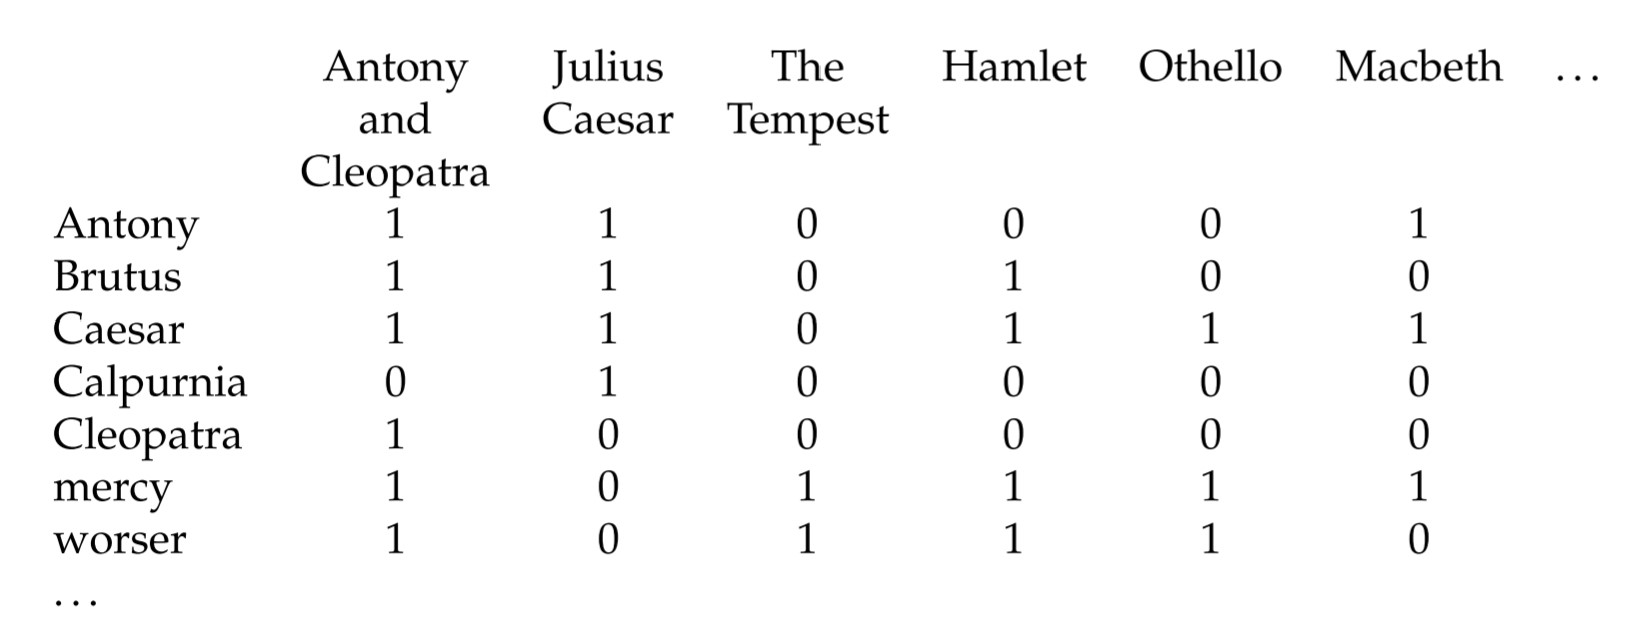
\includegraphics[scale = 0.6]{img/incidence matrix.jpg}
		\label{inc_mat}
\end{figure}

In this matrix, for each term we have a binary vector representing the set of documents including the term. Using this representation, we can answer the previous query by computing a bitwise AND between the vectors of \textit{Brutus}, \textit{Caesar} and \textit{Calpurnia} (complemented). The result is: 110100 AND 110111 AND 101111 = 100100, i.e. the plays that satisfy the query are \textit{Antony and Cleopatra} and \textit{Hamlet}.

In this sense, a \textbf{Boolean retrieval model} is a model for information retrieval in which we can pose any query which is in the form of a Boolean expression of terms, that is, in which terms are combined with the operators AND, OR, and NOT. In this model each document is represented by just using a set of words.

Let's consider a more realistic scenario, and suppose that we have a collection composed of $N = 1$ million documents, each of which is in turn composed of 1000 words (so 1G words in total). If we assume an average of 6 bytes per word, then the size of the collection is 6GB, and if there are $M = 500K$ distinct terms among the collection, then the matrix would have a dimension 500K x 1M. Moreover, since the collection only contains 1G of words, the matrix would be extremely sparse. For this reason, the matrix representation is not feasible for real world data dimension, so a much better representation is given by storing for each term only the documents in which that term appears. This approach can be implemented using the inverted index.

\subsection{Inverted Index}
As introduced before, the idea of the \textbf{inverted index} structure is that for each term $t$, we only store a list of all the documents that contain $t$, the so called postings list. 

\begin{figure}[h!]
		\centering
		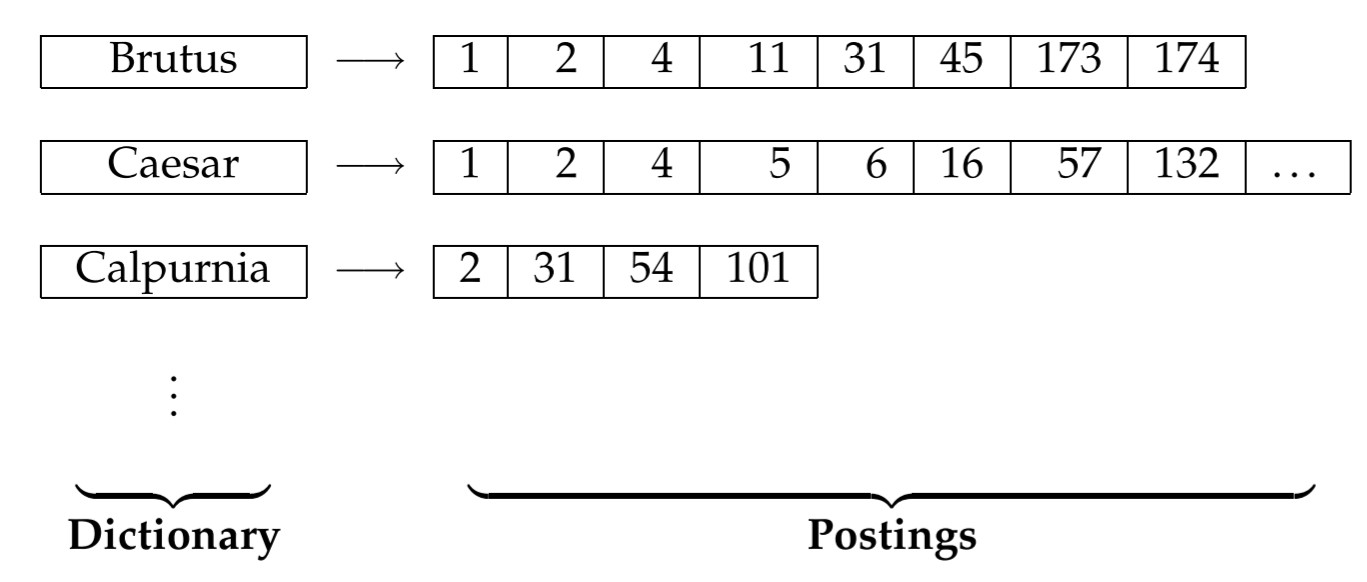
\includegraphics[scale = 0.6]{img/inverted index.jpg}
		\label{inc_mat}
\end{figure}

Usually, the dictionary is stored in the memory, with pointers to each postings list, which is stored on disk. The inverted index construction follows the following steps:

\begin{enumerate}
    \item Collect the documents to be indexed;
    \item Tokenize the text, turning each document to a list of tokens;
    \item Apply some linguistic preprocessing in order to obtain the indexing terms (ex: stemming, removing stop words, etc..);
    \item Create the inverted index combining dictionary and postings.
\end{enumerate}

An example of this building process in represented in Picture \ref{inc_ex}

\begin{figure}[h!]
		\centering
		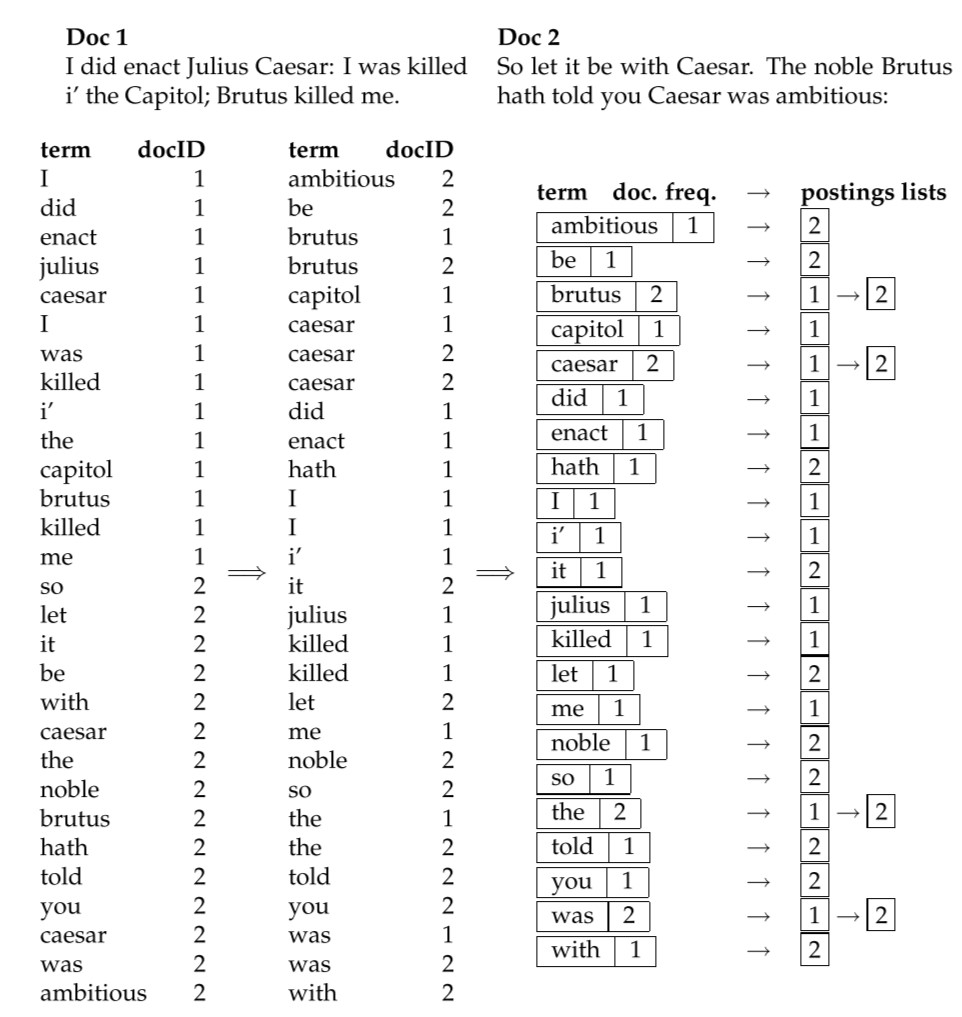
\includegraphics[scale = 0.8]{img/example_inverted index.jpg}
		\label{inc_ex}
\end{figure}

As we can see in the example, the terms of the dictionary are sorted in alphabetical order, and for each term the document frequency information, i.e. the length of its postings list, is added for each term, and it can be helpful for improving the efficiency of the search engine at query time. Since both the dictionary and the postings list are stored, their size is important. Concerning the postings list, a fixed length array would be wasteful as some words occur in many documents, and others in very few, so two good alternatives are \textbf{singly linked lists} or \textbf{variable length arrays}. However, variable length arrays win in space requirements by avoiding the overhead for pointers and in time requirements because their use of contiguous memory increases speed on modern processors with memory caches.

\subsection{Processing boolean queries}
Now the question is: how do we process a query using the inverted index structure and the boolean retrieval model? In we consider the query "\textit{Brutus} AND \textit{Caesar}", then the result can be obtained with the following steps:

\begin{enumerate}
    \item locate \textit{Brutus} in the dictionary;
    \item locate \textit{Caesar} in the dictionary;
    \item compute the intersection of the two postings lists;
\end{enumerate}

\begin{figure}[h!]
		\centering
		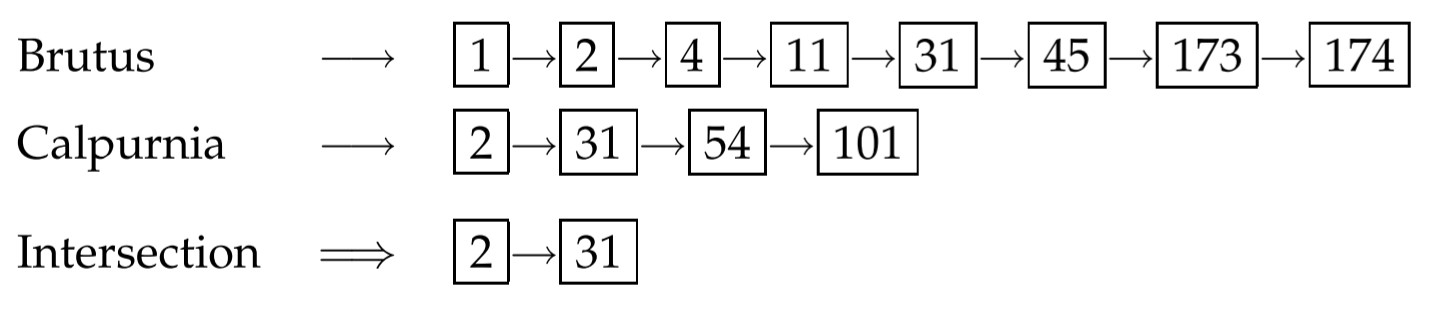
\includegraphics[scale = 0.8]{img/boolean query_inv.jpg}
		\label{inc_ex}
\end{figure}

As we can imagine, the intersection (or merging) operation is crucial: it must be able to retrieve in a fast way the documents that contain both terms. A possible implementation of the intersection operation is represented in Picture \ref{intersection}: in this case the complexity of the operation is $O(x + y)$, where $x$ and $y$ are the lengths of the two postings lists. Note that a crucial assumption of this implementation is that the two lists are sorted.

\begin{figure}[h!]
		\centering
		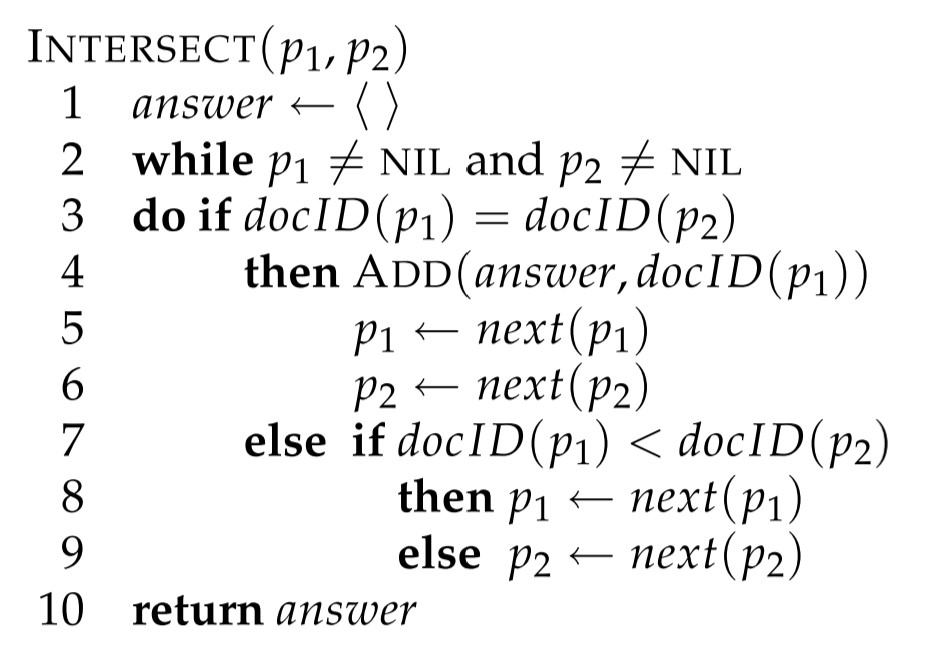
\includegraphics[scale = 0.8]{img/intersection.jpg}
		\label{intersection}
        \caption{Basic implementation of the intersection operation}
\end{figure}

One possible way to speedup the intersection operation is represented by the usage of the \textit{postings list with skip pointers} data structure, as shown in Picture \ref{postings with skip}. Skip pointers are effectively shortcuts that allow us to avoid processing parts of the postings list that will not figure in the search results: at each position of the postings list we can either process the following element or use the pointer to skip irrelevant elements. 

\begin{figure}[h!]
		\centering
		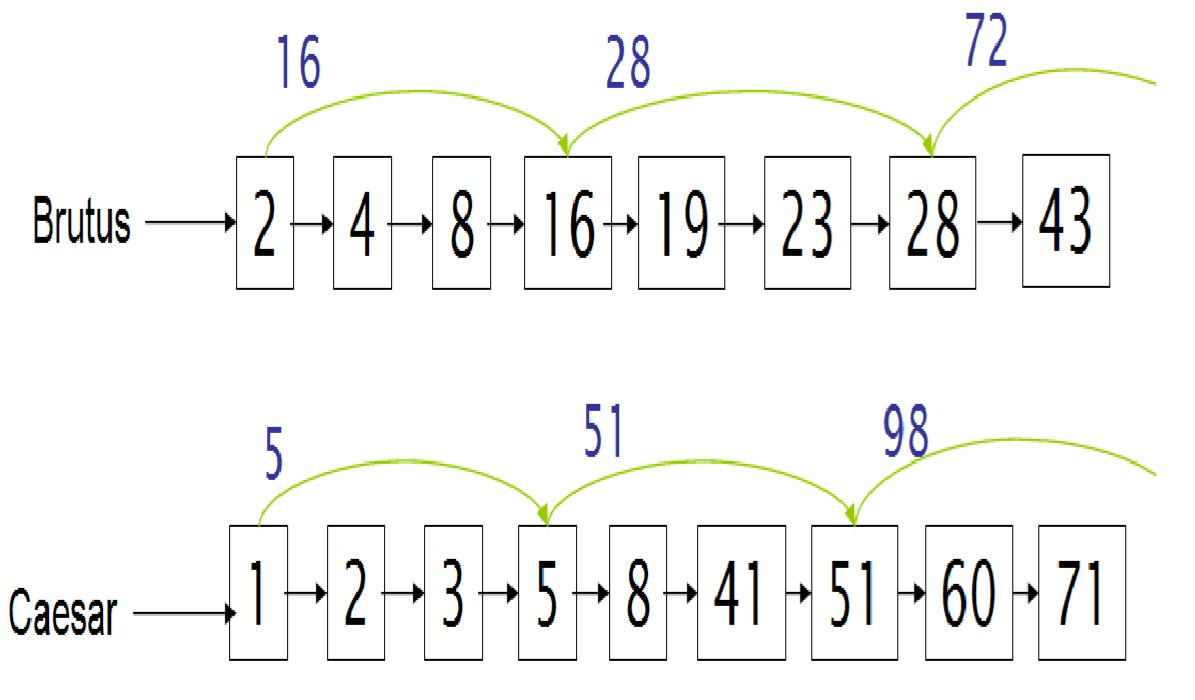
\includegraphics[scale = 0.5]{img/postings with skip.jpg}
		\label{postings with skip}
        \caption{Postings list with skip pointers}
\end{figure}

Now the two questions are \textbf{where} to place skip pointers and \textbf{how} to do efficient merging using skip pointers. Suppose we're considering the two postings lists of Picture \ref{postings with skip}, and that we have matched 8 on each list: we advance both pointers and we reach 16 in the first list, and 41 in the second. Now, since the skip list pointer points to 28, which is still less than 41, we can exploit it to jump directly to 28, without processing 19, and 23. Notice that this is possible thanks to the assumption that the lists are sorted. An example of \textbf{algorithm} that implements the merge operation using the postings lists with skip pointers is shown in Picture \ref{posting intersection with skip}.

\begin{figure}[h!]
		\centering
		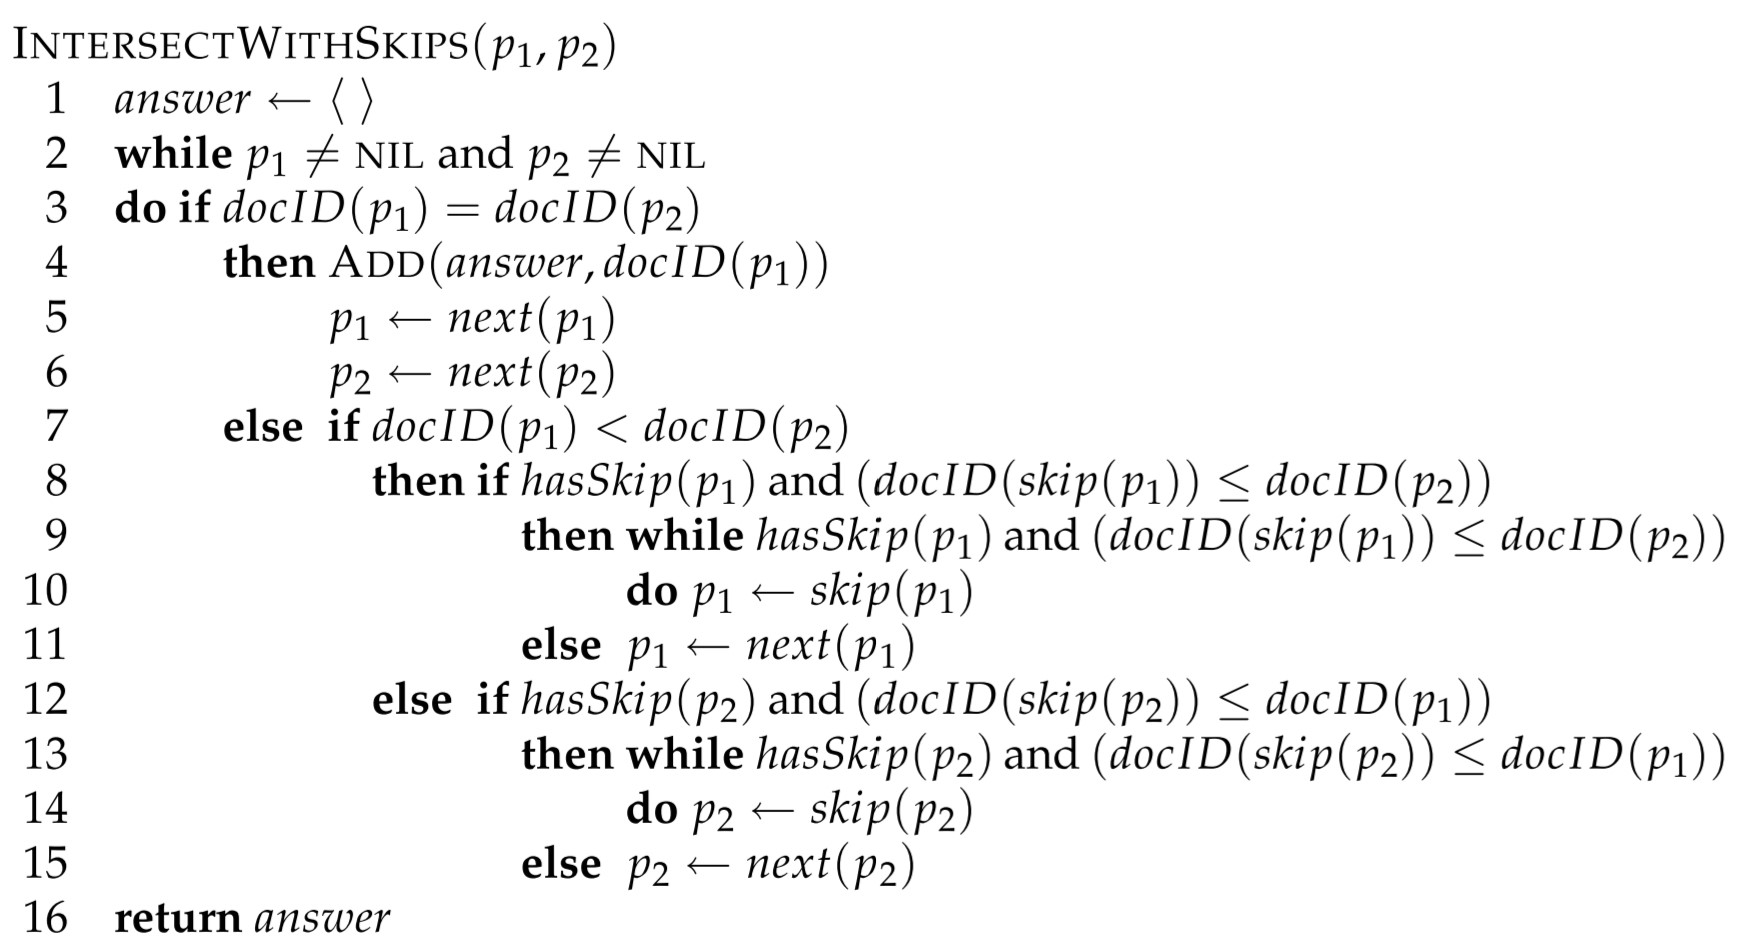
\includegraphics[scale = 0.6]{img/posting intersection with skip.jpg}
		\label{posting intersection with skip}
        \caption{Postings lists intersection with skip pointers}
\end{figure}

Regarding the \textbf{place} in which inserting the skip pointers, there's a \textbf{trade-off} between the number of pointers and the space that they occupy. On the one hand, the more skip pointers, the shorter the skip spans will be, resulting in many comparisons to skip pointers and a lot of space used to store them. On the other hand, the fewer skip pointers, the longer the skip spans will be, resulting in less opportunities to skip and, consequently, in less successful skips. A simple \textbf{heuristic} indicates that for postings list of length $P$ we should use $\sqrt{P}$ evenly-spaced skip pointers, ignoring the distribution of query terms.

In general, building effective skip pointers is easy if an index is relatively static, but it is harder if a postings list keeps changing because of updates.

\subsection{Properties}
Among the advantages, we underline:

\begin{itemize}
    \item It is \textbf{precise}, if the right strategies for searching are known;
    \item It is \textbf{efficient} for computers.
\end{itemize}

On the other hand, the disadvantages are:

\begin{itemize}
    \item The user must learn the \textbf{boolean logic};
    \item The \textbf{boolean logic} is \textbf{insufficient} to capture the \textbf{richness of the language};
    \item There's \textbf{no control} over the \textbf{size of the result set}: either too many or none documents are returned. Moreover, \textbf{all} the documents in the results are considered \textbf{equally good}, i.e. there's no rank for the documents in the solution;
    \item It \textbf{does not support partial matches}.
\end{itemize}

\subsection{Query optimization}
An important issue about \textit{Boolean retrieval model} is represented by understanding which is the best order for query processing. Suppose we're dealing with the following query \textit{Brutus} AND \textit{Calpurnia} AND \textit{Caesar}: for each term we have to get their postings and AND them together. In this case, the best choice would be to process the postings in order of increasing frequency, i.e. start with the smallest postings, by exploiting the document frequency information which is stored. By following this approach, the \textit{intersect} operation is implemented as shown in Picture \ref{sort_intersect}.

\begin{figure}[h!]
		\centering
		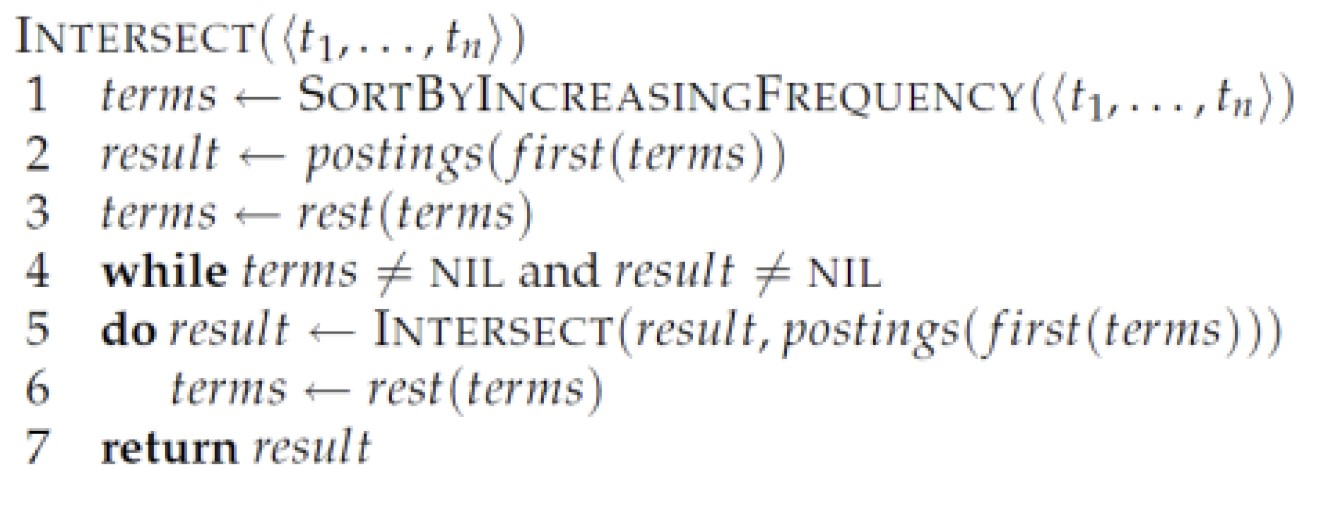
\includegraphics[scale = 0.6]{img/sort_intersect.jpg}
		\label{sort_intersect}
\end{figure}

If we consider another query, for example (\textit{Brutus} OR \textit{Caesar}) AND NOT (\textit{Anthony} OR \textit{Cleopatra}) AND (\textit{Brutus} OR \textit{Cleopatra}), then another approach to speedup the query could be estimate the size of each OR operation by the sum of its document frequencies, and then process in increasing order of the OR sizes.

\subsection{Positional postings and phrase queries}
Most recent search engines support a double quotes syntax (\textit{“stanford university”}) for \textbf{phrase queries}, which has proven to be very easily understood and successfully used by users, as 10\% of web queries are phrase queries, and many more are implicit phrase queries (such as person names), entered without use of double quotes. 

To be able to support such queries, it is no longer sufficient for postings lists to be simply lists of documents that contain individual terms. In this section we consider three approaches to supporting phrase queries and their combination in an efficient way.

\subsubsection{Biword indexes}
One approach could be considering each pair of consecutive terms (biword) in a document as a phrase: for example, the text \textit{"Friends, Romans, Countrymen"} would generate two biwords: \textit{"friends romans"} and \textit{"romans countrymen"}. Each of the \textbf{biword} is now a \textbf{dictionary term}, so in this particular case we would be able to solve a two-word phrase query processing in an immediate way. In general, longer queries can be processed by breaking them down: for example the query \textit{"stanford university palo alto"} can be broken into the following boolean query on biwords: \textit{"stanford university"} AND \textit{"university palo"} AND \textit{"palo alto"}. 

Two important issues about biwords are:

\begin{itemize}
    \item There can be some \textbf{false positives}: without examining the documents, we cannot verify that the documents matching the Boolean query do actually contain the original word phrase;
    \item The problem of the \textbf{index blowup} due to bigger dictionaries.
\end{itemize}

For these reasons, the biword index is not the standard solution, but it can be part of a compound strategy.

\subsubsection{Positional indexes}
This approach is most commonly employed, and it is based on the idea of storing, for each term in the vocabulary, the postings of the form docID: <position1, position2, .., >, where each position is a token index in the document. Each posting will also usually record the term frequency. An example of positional index is provided in Picture \ref{pos_index}: as we can see, for each term, the term frequency is indicated, along with the term frequencies and the positions for each document. In this case, \textit{to} has a document frequency of 993,427, and it appears 6 times in document 1 at positions 7, 18, etc..

\begin{figure}[h!]
		\centering
		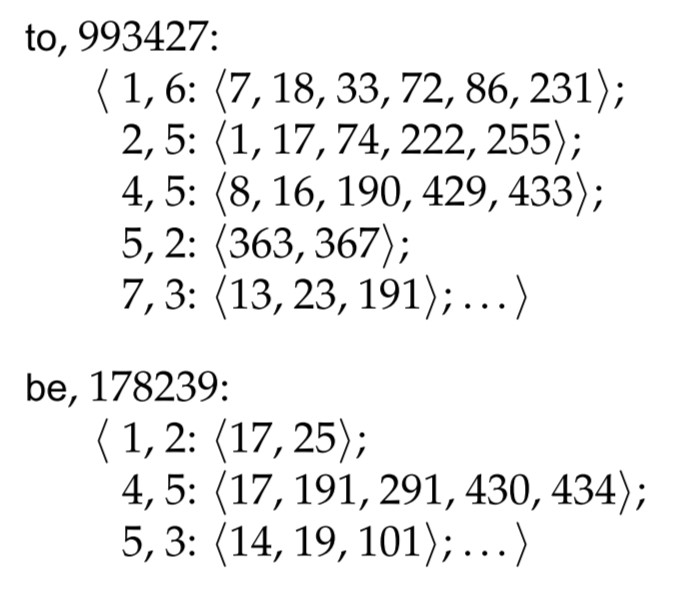
\includegraphics[scale = 0.8]{img/positional_index.jpg}
		\label{pos_index}
        \caption{Positional index}
\end{figure}

To process a phrase query, we still need to access the inverted index entries for each distinct term. As before, we would start with the least frequent term and then work to further restrict the list of possible candidates. In the \textbf{merge operation}, the same general technique is used as before, but rather than simply checking that both terms are in a document, we also need to \textbf{check} that \textbf{their positions} of appearance in the document are compatible with the phrase query being evaluated. This requires working out offsets between the words. For example, suppose that the positional index for the words \textit{to} and \textit{be} are the ones in Picture \ref{pos_index}, and that the query is \textit{to be or not to be}  in this case we first look for the documents that contain both terms, in this case doc1, doc4 and doc5. Then, we look for places in the lists where there is an occurrence of \textit{be} with a token index one higher than a position of \textit{to}, and then we look for another occurrence of each word with token index 4 higher than
the first occurrence. In the above list, these conditions are guaranteed for doc4, since \textit{to} appears in positions 429 and 433, while \textit{be} appears in positions 430 and 434. Notice that doc4 represents a good candidate for solving the query, but an additional check must be performed for terms \textit{or} and \textit{not}.

In general, positional indexes allow to solve $k$ word proximity searches, i.e. searches in which we fix a windows, while biword indexes cannot. Picture \ref{pos_intersect} shows an algorithm for implementing the $k$ word proximity searches: the algorithm finds places where the two terms appear within $k$ words of each other and returns a list of triples giving docID and the term position in $p1$ and $p2$.

\begin{figure}[h!]
		\centering
		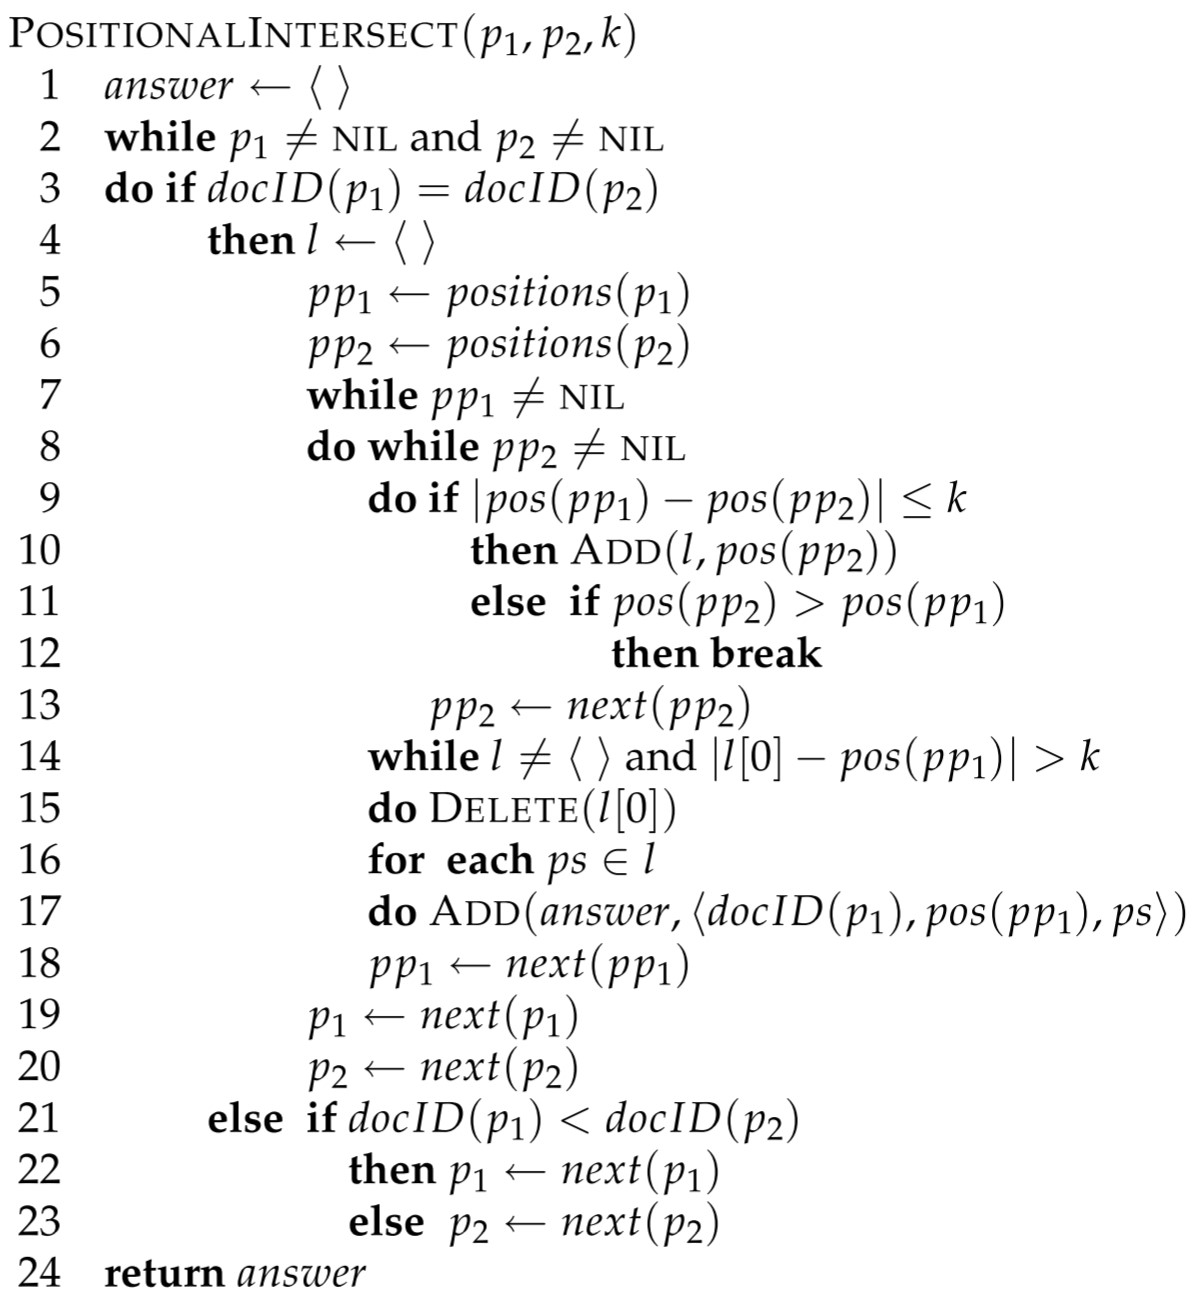
\includegraphics[scale = 0.8]{img/positional_intersect.jpg}
		\label{pos_intersect}
        \caption{Algorithm for proximity intersection of two postings lists}
\end{figure}

A positional index \textbf{expands postings storage substantially}, even if the positions/offsets are compressed. Indeed, the asymptotic complexity of a postings intersection operation is no longer bounded by the number of documents $N$, but by the total number of tokens in the document collection $T$. However, positional indexes are now \textbf{standardly used}, because of the power and usefulness of phrase and proximity queries. From the point of view of space implication, since a posting needs an entry for each occurrence, the \textbf{index size} depends on the \textbf{average document size}: the average web page has less than 1000 terms, but financial documents, books etc.. may easily reach 100,000 terms. If we consider an average term frequency of 0.1\%, then large documents cause an increase of two orders of magnitude in the space required to store the postings list, as represented in Picture \ref{space_pos_index}.

\begin{figure}[h!]
		\centering
		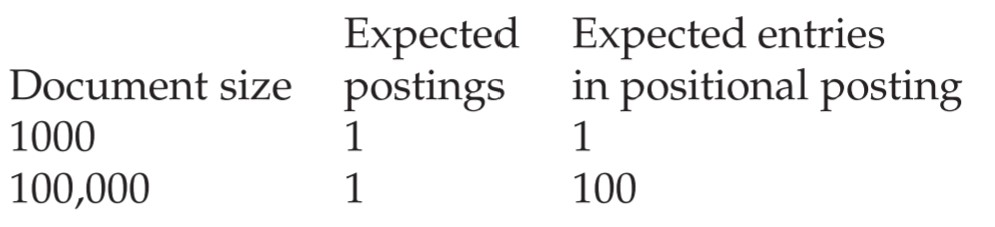
\includegraphics[scale = 0.8]{img/space positional indexes.jpg}
		\label{space_pos_index}
        \caption{Average number of positional postings with different document sizes}
\end{figure}

In general, according to some rules of thumb, a positional index is 2 to 4 times as large as a non-positional index, and a compressed positional index is about one third to one half the size of the raw text (after removal of markup, etc.) of the original uncompressed documents.

\subsubsection{Combination schemes}
This strategy combines the biword and the positional indexes approach, since it uses a phrase index, or just a biword index, for certain queries and uses a positional index for other phrase queries. The idea behind this approach is that it is usually inefficient to keep on merging positional postings lists, so for this reason the most common queries are included in the phrase index. Williams et al. (2004) evaluated a more sophisticated mixed indexing scheme, composed of biwords and positional indexes, and a typical web query mixture was executed in one-fourth of the time of using just a positional index. However, it required 26\% more space than having a positional index alone.


\section{The term vocabulary} \label{ch3}
We recall that the main steps for constructing an inverted index are:

\begin{enumerate}
    \item Collect the documents;
    \item Tokenize the text;
    \item Do some linguistic pre-processing of the tokens;
    \item Create the inverted index.
\end{enumerate}

In this chapter we first examine the possible formats and aspects of the input document, and then we will focus on the steps of tokenization and linguistic pre-processing of them.

\subsection{Documents}
Digital documents that are the input to an indexing process are typically bytes in a file or on a web server. The first step of processing is then to convert this byte sequence into a linear sequence of characters: however, many formats for the input file exist, along with many different encoding in which the convertion can take place. In this sense, the problem of choosing the best encoding could be addressed by a machine learning algorithm, but it is usually handled heuristically. Moreover, there exist some open source libraries that can handle the presence of multiple languages and formats in a document. Finally, the last issue regards the granularity of the documents: in particular, there's a trade-off between precision of the IR system and the recall. If the units get too small, we are likely to miss important passages because terms were distributed over several mini-documents, while if units are too large we tend to get spurious matches and the relevant information is hard for the user to find. In the following sections we assume that a suitable document size is chosen.

\subsection{Tokenization}
Given a character sequence and a defined document unit, \textbf{tokenization} is the task of chopping it up into pieces, called \textit{tokens}, perhaps at the same time throwing away certain characters, such as punctuation. Despite being often called \textit{terms} or \textit{types}, there's a difference between these entities:

\begin{itemize}
    \item a \textit{token} is an instance of a sequence of characters in some particular document that are grouped together as a useful semantic unit for processing;
    \item a \textit{type} is the class of all tokens containing the same character sequence;
    \item a \textit{term} is a (perhaps normalized) type that is included in the IR system’s dictionary.
\end{itemize}

For example, if the document to be indexed is \textit{to sleep perchance to dream}, then there are 5 tokens, but only 4 types (since there are two instances of \textit{to}). 

Now the question is: what are the correct tokens to use? How do we extract them? In general, for each language there are some tricky cases (e.g. if we have \textit{aren't}, we could tokenize it into \textit{are} and \textit{n't} or \textit{aren} and \textit{t} etc..), and for this reason the \textbf{issues} of tokenization are \textbf{language-specific}. Some examples of issues of tokenization are (more on Chapter 2 of the book):

\begin{itemize}
    \item How to split ambiguous words (e.g. \textit{aren't}, \textit{O'Neill} etc..);
    \item How to deal with special types of characters, such as e-mail addresses, web URLs, IP addresses etc.. A possible solution could be represented by omitting them, resulting on the other hand in restricting a lot what people could search for;
    \item In English, \textit{hyphenation} is a popular technique for splitting up vowels in words or for joining nouns as names; however, handling hyphens automatically could be hard, and it usually done in an heuristic way;
    \item Other language-specific issues (e.g. French, German, Chinese etc..).
\end{itemize}

\subsection{Stop words}
We define \textbf{stop words} as extremely common words (around 30\%) that would appear to be of little value in helping selecting documents matching a user need. The general strategy for determining a \textit{stop list} is to sort the terms by collection frequency, and then to take the most frequent terms and discard them. The usage of the stop list allows both to significantly \textbf{reduce the number of postings} that the system has to store and to save a lot of time in the indexing phase. However, in some cases the stopwords are very useful, for example in the \textit{phrase queries}, such as \textit{President of United States}, in \textit{relational queries}, such as \textit{Flights to Venice} or in some song titles, for example \textit{Let it be}.

The general trend in IR systems over time has been from standard use of quite large stop lists (200–300 terms) to very small stop lists (7–12 terms) to \textbf{no stop list} whatsoever. Web search engines generally do not use stop lists.

\subsection{Normalization}
Having broken up our documents (and also our query) into tokens, the easy case is if tokens in the query just match tokens in the token list of the document. However, there are many cases when two character sequences are not quite the same but you would like a match to occur. For instance, if you search for \textit{USA}, you might hope to also match documents containing \textit{U.S.A}. In this sense, \textit{token normalization} is the process of canonicalizing tokens so that matches occur despite superficial differences in the character sequences of the tokens. The most standard way to normalize is to implicitly create \textbf{equivalence classes}, which are normally named after one member of the set. For instance, if the tokens \textit{anti-discriminatory} and \textit{antidiscriminatory} are both mapped onto the term \textit{antidiscriminatory}, in both the document text and queries, then searches for one term will retrieve documents that contain either. 

Another issue about tokenization is represented by \textbf{accents} and \textbf{diacritics}, which in some languages are a regular part of the writing system and distinguish different sounds and meanings. In these cases, the important question is how the users are likely to write their queries for these words: even in languages that standardly have accents, users often may not type them (lazyness, speed etc..). In these cases, it might be the best to equate all words to a form without diacritics. A common strategy is to do \textbf{case-folding} by reducing all letters to lower case: in this case, all the terms will be retrieved, regardless of the correct capitalization. However, such case folding could equate words that might be better be kept apart, for example \textit{General Motors}, \textit{Fed} etc..

\subsection{Stemming and Lemmatization}
The goal of both \textbf{stemming and lemmatization} is to \textbf{reduce inflectional forms} and sometimes of derivationally related forms of a word to a common base form. For instance, \textit{am, are} and \textit{is} become \textit{be}: if we apply this to a sentence, \textit{the boy's car are of different colors} becomes \textit{the boy car be different color}. However, there'a little difference between stemming and lemmatization:

\begin{itemize}
    \item \textit{Stemming} usually refers to a crude heuristic process that chops off the ends of words in the hope of achieving this goal correctly most of the time, and often includes the removal of derivational affixes;
    \item \textit{Lemmatization} usually refers to doing things properly with the use of a vocabulary and morphological analysis of words, normally aiming to remove inflectional endings only and to return the base or dictionary form of a word, which is known as the \textit{lemma}.
\end{itemize}

The most common \textbf{algorithm for stemming English}, which have been shown to be empirically effective, is \textbf{Porter's algorithm}. This algorithm consists of 5 phases of word reductions applied sequentially, and each phase consists of a set commands: the usual convention is to select the command that applies the longest suffix. Picture \ref{porter} shows the set of commands of the first phase.

\begin{figure}[h!]
		\centering
		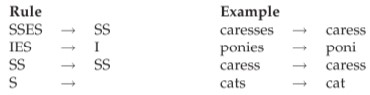
\includegraphics[scale = 1.8]{img/porter.jpg}
		\label{porter}
        \caption{Set of commands of the first phase}
\end{figure}

Many of the later rules use the concept of the \textit{measure} of a word, i.e. they check the number of syllables to see whether a word is long enough that is reasonable to regard the matching portion of a rule as a suffix rather than as part of the stem of a word. For example, the rule \textit{(m > 1) EMENT} would map \textit{replacement} to \textit{replac}, but not \textit{cement} to \textit{c} (since the prefix \textit{c} is not long enough).

In general, stemmers use language-specific rules, but they require less knowledge than a lemmatizer, which needs a complete vocabulary and morphological analysis to correctly lemmatize word. The \textbf{advantages} of performing stemming is that it helps increasing the \textbf{recall} of the IR system, i.e. the amount of its results, but on the other hand it could harm the precision, i.e. the quality of the results, of other IR system. In general, this operation helps on reducing the size of the vocabulary, and it was shown that is very useful for languages with much more morphology, such as Spanish, German and Finnish.

\section{Dictionaries and Tolerant Retrieval}\label{ch4}
In Chapters \ref{ch2} and \ref{ch3} we developed the ideas underlying inverted indexes for handling Boolean and proximity queries, so now we develop techniques that are robust to typographical errors in the query, as well as alternative spellings (tolerant retrieval).

In section \ref{4.1} we develop data structures that help the search of terms in the vocabulary in an inverted index, in Section \ref{4.2} we study the idea of \textit{wildcard queries}, that are used when the user is uncertain of the spelling of a query term, while in Section \ref{4.3} we focus on spelling errors.

\subsection{Search structures for dictionaries}\label{4.1}
Given an \textbf{inverted index} and a \textbf{query}, our first task is to determine whether each query term exists in the vocabulary and if so, identify the pointer to the corresponding postings. This operation is usually implemented by exploiting the \textbf{vocabulary} data structure: in our case, the dictionary stores the term vocabulary (representing the \textit{keys} of the dictionary), its document frequency and the pointer to the corresponding posting list. Usually, a vocabulary is implemented by using \textbf{hash tables} or \textbf{search trees}, and the choice between the two solutions depend on many factors, for example the number of keys that we have, whether this number is likely to change or not, the relative frequencies of each key etc..

\subsubsection{Hash Tables}
In the \textbf{hashing} technique, each vocabulary term is hashed into an integer (we assume that this operation minimizes the collisions), which is then used to access the corresponding posting list. The main \textbf{advantage} of this solution is that the vocabulary lookup is very fast, $O(1)$. However, there are several \textbf{disadvantages}: the hash table does not provide an easy way to find minor variants of the term, since different terms results in two different integers, and does not allow to search for a term using the prefix (tolerant retrieval). Finally, one important issue is that if the vocabulary keeps growing, a re-hashing operation of the whole vocabulary must be done, and this is usually very expensive.

\subsubsection{Search Trees}
\textbf{Search trees} are data structures that overcome some of the issues of the hash tables. The best-known search tree is the \textit{binary tree}, in which each internal node has two children, and it can be considered as a binary test that affects the search for a term, in the sense that the outcome of the test determines one of the two sub-trees along which the search proceeds. Picture \ref{binary tree} gives an example of binary tree used for a dictionary.

\begin{figure}[h!]
		\centering
		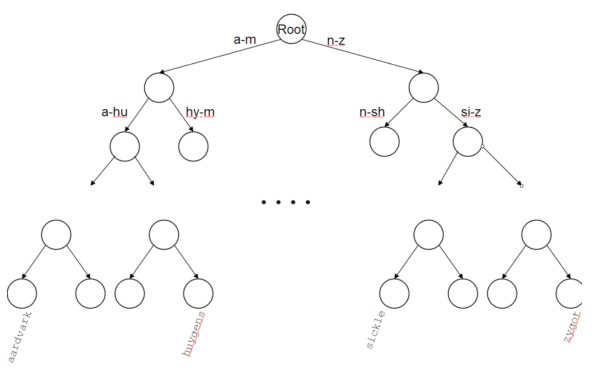
\includegraphics[scale = 1.8]{img/binary tree.jpg}
		\label{binary tree}
        \caption{Binary tree for a dictionary}
\end{figure}

The main issue about binary trees is that in order to implement efficient search, i.e. with complexity $O(logM)$, the tree must be \textbf{balanced}, so a big disadvantage of this structure is given by the overhead of maintaining the tree balanced when a new document is inserted.

To overcome this problem, usually the \textbf{B-tree} data structure is used: the \textit{B-tree} is a generalization of the binary tree in which every internal nodes has a number of children in the interval $[a,b]$, where $a$ and $b$ are appropriate natural numbers. Picture \ref{b tree} shows a B-tree where $a = 2$ and $b = 4$. We notice that, because a range of child nodes is permitted, B-trees do not need re-balancing as frequently as binary trees, but on the other hand they may waste more space when the nodes are not entirely full.

\begin{figure}[h!]
		\centering
		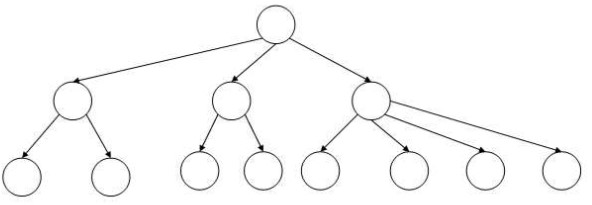
\includegraphics[scale = 1.8]{img/b tree.jpg}
		\label{b tree}
        \caption{B-tree for a dictionary}
\end{figure}

In general, the simplest search tree to implement is the \textit{binary tree}, but \textit{B-trees} are the most used. We notice that trees, unlike hash tables, require a \textbf{standard ordering} of the characters, which is usually represented by the \textit{lexicographic order}. The \textbf{advantage} of using the \textit{search trees} is that they solve the prefix problem, i.e. they allow to search for a term by providing its prefix. The \textbf{disadvantages} are that they are usually slower than hash tables ($O(log M)$ vs $O(1)$), and they may require the re-balancing operation, which is quite expensive, although the B-trees mitigate this problem.

\subsection{Wildcard queries}\label{4.2}
As we introduced before, the wildcard queries can be used when the user is uncertain of the spelling of a query, or when the user wants to retrieve documents containing all the variants of a term etc..

An example of wildcard query is \textit{mon*}, and it is called \textbf{trailing wildcard query}, since the symbol * occurs only once at the end of the string. This type of wildcard query is quite simple to be answered by using a binary tree (or B-tree) lexicon, since we have to search for all the words s.t. $\text{mon} \leq \text{word} \leq \text{moo}$, by traversing the tree.

A slight generalization of this typology is the \textbf{leading wildcard query}, where the queries are in the form \textit{*mon}: these queries can be answered by maintaining an additional reverse B-tree that stores the terms backwards.

Finally, we can handle an even more general case: wildcard queries in which there is a single * in the middle of the query, such as \textit{co*tion}. To solve these queries, we use the regular B-tree to retrieve the set of terms beginning with the prefix \textit{co}, then we use the reverse B-tree to retrieve the set of terms ending with the suffix \textit{tion}, and finally we intersect the two term sets using the standard inverted index. Obviously, this solution is quite expensive, and for this reason a possible improvement can be brought by transforming the wildcard queries so that the *'s occur always at the end of the terms. This approach gives rise to the \textbf{permuterm index}.

\subsubsection{Permuterm index}
The \textbf{permuterm index} is a form of inverted index in which all the possible permutations of a term all link to the original vocabulary term, as represented in Picture \ref{permuterm_index}. Notice that the character \$ is a special symbol that marks the end of a term: this character increases the vocabulary size, since we now store $n+1$ terms, where $n$ is the term size, rather than just 1. The set of rotated terms in the permuterm index is called \textit{permuterm vocabulary}.

\begin{figure}[h!]
		\centering
		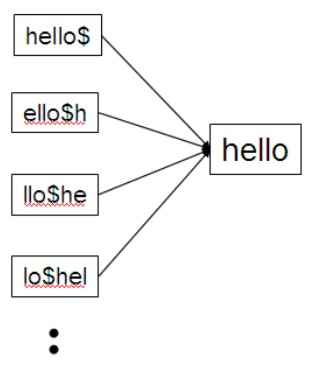
\includegraphics[scale = 1.6]{img/permuterm index.jpg}
		\label{permuterm_index}
        \caption{A portion of a permuterm index}
\end{figure}

As we introduced before, the goal of the \textit{permuterm index} is to rotate the wildcard query so that the * symbol appears at the end of the string. For example, if the query is \textit{h*e}, we insert the symbol \$, so \textit{h*e\$}, and our goal is to consider the term \textit{e\$h*}. Finally we can search the terms starting with \textit{e\$h*} using a standard B-tree lookup to retrieve the matching documents.

Now the problem is how to handle wildcard queries containing multiple * symbols, such as \textit{fi*mo*er}.  In this case we first enumerate the terms in the dictionary that are in the permuterm index of \textit{er\$fi*}. Not all such dictionary terms will have the string \textit{mo} in the middle, so we filter these out by exhaustive enumeration, checking each candidate to see if it contains \textit{mo}. Finally, we run the surviving terms through the standard inverted index for document retrieval.

One \textbf{disadvantage} of the permuterm index is that its dictionary becomes like 4 to 10 times larger than the original one, so we now introduce another method to answer wildcard queries.

\subsubsection{$k$-gram indexes for wildcard queries}
A $k$-gram is a sequence of $k$ characters, so \textit{cas}, \textit{ast} and \textit{stl} are all 3-grams occurring in the term \textit{castle}. We use a special character \$ to denote the beginning or end of a term, so the full set of 3-grams generated for castle is: \textit{\$ca}, \textit{cas}, \textit{ast}, \textit{stl}, \textit{tle}, \textit{le\$}. 

In the \textit{$k$-gram index}, the vocabulary contains all the $k$-grams that occur in any term in the vocabulary, and each postings list of a $k$-gram contains all the terms containing the corresponding $k$-gram. An example is provided in Picture \ref{kgram}.

\begin{figure}[h!]
		\centering
		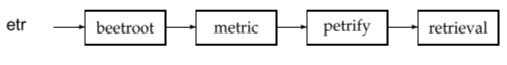
\includegraphics[scale = 1.6]{img/k-grams .jpg}
		\label{kgram}
        \caption{Postings list of a $k$-gram}
\end{figure}

Now, this particular index can be used for solving wildcard queries in the following way: suppose that the query is \textit{re*ve}, we then run the Boolean query \textit{\$re} AND \textit{ve\$}, and each of the matching terms is then looked up in the standard inverted index to yield documents matching the query. However, this approach leads to the retrieval of some \textbf{false positives}. Consider for example the query \textit{red*}: following the approach described above, we would perform the Boolean query \textit{\$re} AND \textit{red}, but this would lead to match terms like \textit{retired}, which is a false positives w.r.t. the original query. In this sense, a \textbf{post-processing} phase must be introduced, in order to filter the false positives against the original query: the surviving terms are then looked up in the standard inverted index.

\subsubsection{Permuterm index vs $k$-gram index}
As we said before, \textbf{permuterm index} is not space efficient: if $n$ is the average length of a word, using the character \$ as a suffix, we add $n$ rotations to the vocabulary; overall, we need $(n+1) * (n+1)$ chars for a term of $n$ chars.

With 2-grams, considering the leading and trailing \$, we use $(n+1) * 2$ chars, where $n+1$ is the number of bigrams for each term considering the symbol \$. Finally, with 3-grams we need $n*3$ chars.

In general, wildcard queries can result in very expensive query execution, and for this reason this capability is hidden behind an interface (say "Advanced Query"), which most users do not use.

\subsection{Spelling correction}\label{4.3}
We now consider the problem of \textbf{spelling correction} in queries, and in particular we focus on two possible solutions: the first one is based on \textit{edit distance}, while the second one on \textit{k-gram overlap}.

In general, the two main uses of the spelling correction are:

\begin{itemize}
    \item correcting the documents being indexed, and in particular this in important if the documents are retrieved using OCR (optical character recognition);
    \item correcting user queries to retrieve the correct answers (\textit{Did you mean..?}).
\end{itemize}

\subsubsection{Forms of spelling correction}
We focus on two specific forms of spelling correction:

\begin{itemize}
    \item \textbf{isolated-term correction}, in which we attempt to correct a single query term at a time. This type of correction does not catch typos resulting in correctly spelled words, e.g. \textit{flew form Heathrow}, since each term in the query is correctly spelled in isolation;
    \item \textbf{context-sensitive correction}, in which the surrounding words are considered. In this case, the mispelling of the previous example is detected.
\end{itemize}

In general, given a lexicon and a char sequence $Q$, the goal of this technique is to return the words in the lexicon closest to $Q$, and, in particular, among alternative correct spellings for a mis-spelled query, choose the "nearest" one. If two correctly spelled queries are tied, then select the most common.

\textbf{\underline{Isolated-term correction}}

We first analyze two techniques for addressing isolated-term correction: edit distance and $k$-gram overlap. 

Given two strings $S_1$ and $S_2$, the \textit{edit distance} (or \textit{Levenshtein distance}) is the minimum number of edit operations to convert one to the other. The operations are typically character-level, and they're usually \textit{insert}, \textit{delete}, \textit{replace} and \textit{transposition}. For example, the \textit{edit distance} between \textit{cat} and \textit{act} is 2, since two replacements are needed. A more accurate measure can be also obtained using the \textit{weighted edit distance}, where different weights are used for different kind of edit operations, depending on the likelihood of letters that are replaced (e.g. $m$ is more likely to be mis-typed as $n$ than as $q$, so replacing $m$ by $n$ is a smaller edit disance than by $q$). In general, the (weighted) edit distance can be computed using dynamic programming with complexity $O(|S_1| \text{x} |S_2|)$, and in the case of the weighted version, a weight matrix must be provided as input to the algorithm.

The spelling correction problem however demands more than computing edit distance: given a set $S$ of strings (corresponding to terms in the vocabulary) and a query string $q$, we seek the string(s) in $V$ of least edit distance from $q$. The obvious way of doing this is to compute the edit distance from $q$ to each string in $V$, before selecting the string(s) of minimum distance: however, this naive solution is quite expensive and extremely slow ($O(n^2)$). For this reason, some heuristics are adopted to cut the set of candidate dictionary terms: 

\begin{itemize}
    \item restrict the search to dictionary terms beginning with the same letter as the query string: in this case we hope that spelling errors do not occur in the first letter of the query;
    \item generate everything up to edit distance $k = 1,2$ and then intersect these candidates with terms in the index lexicon.
\end{itemize}

Another way to limit the set of vocabulary terms for which we compute edit distances to the query term is by using the \textbf{$k$-gram index} that we introduced for wildcard queries. In particular, this index is used to retrieve vocabulary terms that have many $k$-grams in common with the query: for example, the bigram index in Picture \ref{kgram_spelling} shows the postings for the three brigrams of the word \textit{bord}. Suppose that we want to retrieve the vocabulary terms that contain at least two of these bigrams, then a single scan of the postings would result in retrieving \textit{aboard}, \textit{border}, and \textit{boardroom}.

\begin{figure}[h!]
		\centering
		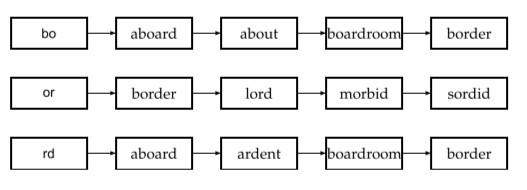
\includegraphics[scale = 1.6]{img/kgram spelling.jpg}
		\label{kgram_spelling}
        \caption{$k$-gram for spelling correction}
\end{figure}

However, we would like to consider a more precise measure of overlap, and one option could be the \textit{Jaccard coefficient}, which is defined as $\frac{|A \cap B|}{|A \cup B|}$, where $A$ and $B$ are, respectively, the set of $k$-grams in the query and the set of $k$-grams in a vocabulary term. As the scan proceeds, we proceed from one vocabulary term $t$ to the next, computing on the fly the \textit{Jaccard coefficient} between $q$ and $t$. If the coefficient exceeds a preset \textbf{threshold}, we add $t$ to the output; if not, we move on to the next term in the postings.

\underline{\textbf{Context-sensitive approach}}

As we underlined before, isolated-term correction would fail to correct typographical errors such as \textit{flew form Heathrow}, where all three query terms are correctly spelled: our desired output would be that the search engine may offer the corrected query \textit{few from Heathrow}. 

The simplest way to do this is to enumerate corrections of each of the three query terms (using the methods we described before) even though each query term is correctly spelled, then try substitutions of each correction in the phrase. For the example \textit{flew form Heathrow}, we enumerate such phrases as \textit{fled form Heathrow} and \textit{flew fore Heathrow}. For each such substitute phrase, the search engine runs the query and determines the number of matching results: finally, the engine suggests the alternative that has lots of hits. Obviously, this enumeration can be expensive if we find many corrections of the individual terms, since we could encounter a large number of combinations of alternatives.

A possible heuristic that can be used for reduce the search space is to retain only the most frequent combinations in the collection or in the query logs, which contain previous queries by the users. For example, we would retain \textit{flew from} as an alternative to try and extend to a three-term corrected query, but perhaps not \textit{fled fore} or \textit{flea form}.


\section{Index construction}\label{ch5}
In this chapter we focus on how to construct an inverted index, i.e. the process of \textit{index construction}.

\subsection{Hardware basics}
When building an information retrieval (IR) system, many decisions are based on the characteristics of the computer hardware on which the system runs. The following list provides the hardware basics that are needed to motivate IR systems.

\begin{itemize}
    \item Access to data in \textbf{memory} is much \textbf{faster} than access to data on \textbf{disk}: consequently, we want to keep as much data as possible in memory, especially those data that we need to access frequently. We call the technique of keeping frequently used disk data in main memory \textbf{caching};
    \item When doing a disk read or write, it takes a while for the disk head to move to the part of the disk where the data are located, and \textbf{no data} are being \textbf{transferred} \textbf{during this seek time}. To maximize data transfer rates, chunks of data that will be read together should therefore be stored contiguously on disk;
    \item Operating systems generally \textbf{read} and \textbf{write} entire \textbf{blocks}. Thus, reading a single byte from disk can take as much time as reading the entire block;
    \item \textbf{Data transfers} from disk to memory are handled by the \textbf{system bus}, not by the processor. This means that the processor is available to process data during disk I/O. We can exploit this fact to speed up data transfers by storing compressed data on disk. Assuming an efficient decompression algorithm, the total time of reading and then decompressing compressed data is usually less than reading uncompressed data;
    \item Servers used in IR systems typically have several \textbf{gigabytes} (GB) of \textbf{main memory}, sometimes tens of GB. Available disk space is several orders of magnitude larger;
    \item \textbf{Fault tolerance} is very \textbf{expensive}, so it is much cheaper to use many regular machines rather than one fault-tolerant machine.
\end{itemize}

In particular, Picture \ref{assumptions} shows the hardware assumptions for this chapter.

\begin{figure}[h!]
		\centering
		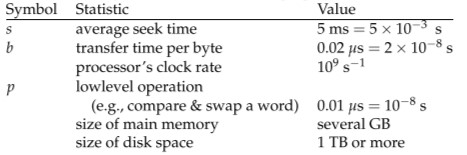
\includegraphics[scale = 1.8]{img/assumptions.jpg}
		\label{assumptions}
        \caption{Hardware assumptions for this chapter}
\end{figure}

\subsection{Blocked sort-based indexing (BSBI)}
The basic steps in constructing an inverted index are represented in Picture \ref{inc_ex}: the first phase is passing through the collection to assemble all the term-docId pairs, then the pairs are sorted and the docIds are organized for each term into a postings list, computing statistics like term and document frequencies. For small collections, all of this can be done in memory, but in this Chapter we analyze some methods for large collections, that require secondary memory storage.

\begin{figure}[h!]
		\centering
		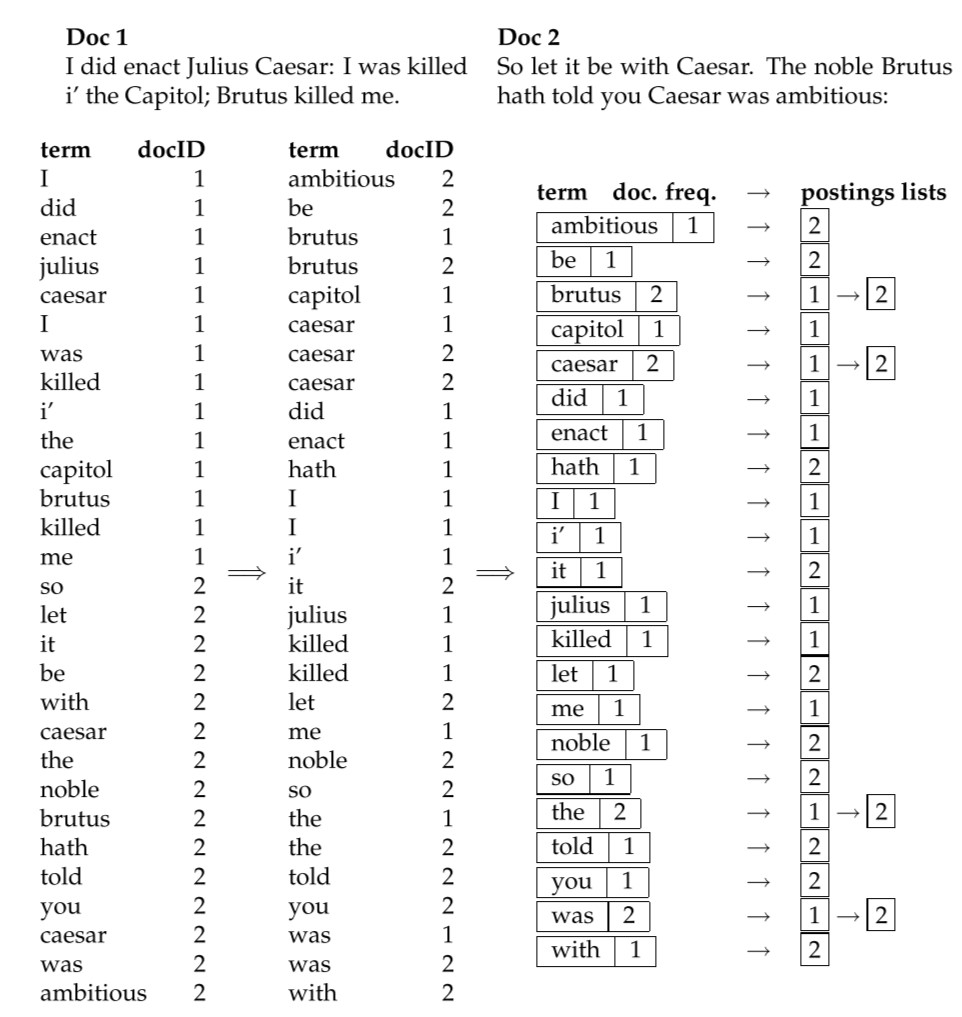
\includegraphics[scale = 0.8]{img/example_inverted index.jpg}
		\label{inc_ex}
\end{figure}

To make index construction more efficient, we represent terms as \textbf{termIDs}, where each termID is a unique serial number, and we work with the \textit{Reuters-RCV1} collection as our model collection in this Chapter, whose statistics are showed in Picture \ref{reuters}.

\begin{figure}[h!]
		\centering
		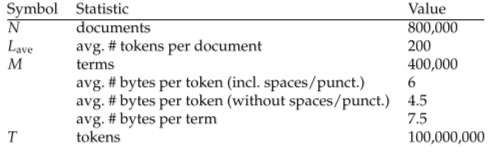
\includegraphics[scale = 1.5]{img/reuters.jpg}
		\label{reuters}
        \caption{Main statistics of \textit{Reuters-RCV1} collection}
\end{figure}

As represented in Picture \ref{inc_ex}, after all the documents have been parsed, the inverted file is sorted by terms. \textit{Reuters-RCV1} contains 100 million tokens, so collecting all termID-docID pairs of the collection using 4 bytes for each pair would require 0.8 GB of storage: clearly, it is not possible to sort them in memory, so we need an \textit{external sorting algorithm}. The main requirement of this algorithm is to minimize the number of random disk seeks during sorting. 

One solution is the \textit{blocked sort-based indexing} algorithm or \textit{BSBI} of Picture \ref{bsbi}. This algorithm:

\begin{enumerate}
    \item Segments the collection into parts of equal size;
    \item Sorts the termID-docID pairs of each part in memory;
    \item Stores the intermediate results on disk;
    \item Merges all intermediate results into the final index.
\end{enumerate}

\begin{figure}[h!]
		\centering
		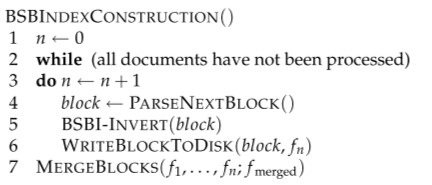
\includegraphics[scale = 1.5]{img/bsbi.jpg}
		\label{bsbi}
        \caption{\textit{BSBI} algorithm}
\end{figure}

Some notes:

\begin{itemize}
    \item The algorithm parses documents into termID–docID pairs and accumulates the pairs in memory until a block of a fixed size is full (function PARSENEXTBLOCK in the code). We choose the block size to fit comfortably into memory to permit a fast in-memory sort;
    \item Then, the termID-docID pairs are sorted;
    \item Next, we collect all termID–docID pairs with the same termID into a postings list, where a posting is simply a docID. The result, an inverted index for the block we have just read, is then written to disk;
    \item Finally, the algorithm simultaneously merges the blocks into one large merged index.
\end{itemize}

If we apply this approach to \textit{Reuters-RCV1} collection, and if we assume that we can fit 10 million termID-docID pairs into memory, we end up with 10 blocks, each of which is an inverted index of one part of the collection. Finally, the blocks are merged into the final index. An example with two blocks is shown in Picture \ref{bsbi example}.

\begin{figure}[h!]
		\centering
		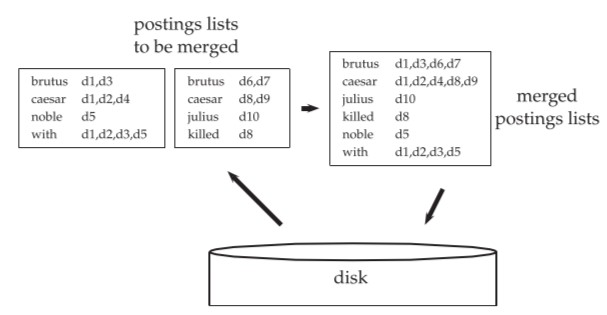
\includegraphics[scale = 1.5]{img/bsbi example.jpg}
		\label{bsbi example}
        \caption{Example of the \textit{BSBI} algorithm}
\end{figure}

One crucial operation of this algorithm is clearly the final \textbf{merge phase}: one possible way to implement it could be by performing a \textbf{binary merge}, but using this strategy we would need to re-write increasingly larger blocks to disk, resulting in a very expensive operation. For this reason, a \textbf{multi-way merge} is preferred, and it consists of opening all the block files simultaneously and maintain small read buffers for the ten blocks we are reading and a write buffer for the final merged index we are writing. By using this technique, we do not perform too many disk seeks, so the algorithm has better performances.

The \textbf{complexity} of \textit{BSBI} algorithm is $\Theta(T log T)$, and it derives by the sorting phase (assuming that we use QuickSort), where $T$ is the number of termID-docID pairs. However, the actual indexing time is dominated by the parsing operation (PARSENEXTBLOCK) and the final merging operation (MERGEBLOCKS). 

Some \textbf{issues} about this algorithm are:

\begin{itemize}
    \item The assumption to use this algorithm is that we're able to keep all the dictionary in memory, and this is not always the case;
    \item Again, the dictionary is needed to produce the mapping from \textit{term} to \textit{termID}: we could also work with term-docID postings, but then the intermediate files would become too large, resulting in a scalable but very slow algorithm.
\end{itemize}

\subsection{Single-pass in-memory indexing (SPIMI)}
The \textit{SPIMI} algorithm is a more scalable alternative to \textit{BSBI} that is based on two key ideas:

\begin{itemize}
    \item It uses terms instead of termID, so no mapping between term and termID is needed across the blocks;
    \item This algorithm does not sort the postings, so the docIDs are generated and assigned sequentially to the documents.
\end{itemize}

Using these two ideas, we can generate a complete inverted index for each block, and then merge them together into one big index. The \textit{SPIMI} algorithm is shown in Picture \ref{spimi}: notice that the part of the algorithm that parses the documents and turns them into term-docID pairs (tokens) is omitted. The algorithm receives in input the token stream, and run until the entire collection has been processed.

\begin{figure}[h!]
		\centering
		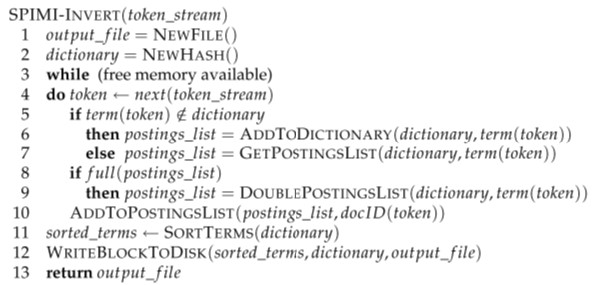
\includegraphics[scale = 1.5]{img/spimi.jpg}
		\label{spimi}
        \caption{\textit{SPIMI} algorithm}
\end{figure}

Some notes:

\begin{itemize}
    \item \textit{Line 4}: each token is processed one at a time;
    \item \textit{Line 5 and 6}: when a term occurs for the first time, it is added to the dictionary and a new empty postings list is created (\textit{Line 6});
    \item \textit{Line 7}: if the term already belongs to the dictionary, the corresponding postings list is retrieved;
    \item \textit{Line 8 and 9}: if the postings list is full, the size is doubled (some memory is wasted);
    \item \textit{Line 10}: the docID of the token is directly inserted into the postings list. Contrary to \textit{BSBI}, where the termID-docID pairs were sorted, here each postings list is dynamic, i.e. its size is adjusted as it grows (\textit{Line 8 and 9}). This approach has two advantages: on the one hand, it is faster since no sorting is required, on the other it saves a lot of memory because the termID of postings need not to be stored;
    \item \textit{Line 11}: when the memory is exhausted, the terms are sorted in order to write the postings lists in lexicographic order, which helps the final merging step;
    \item \textit{Line 12}: the index of the block (dictionary and postings list) is written to disk;
    \item Finally, the blocks are merged (not shown in the picture)
\end{itemize}

Another important feature of this algorithm is \textbf{compression}: both the postings and the dictionary terms can be stored compactly on disk if we employ compression. Compression increases the efficiency of the algorithm further because we can process even larger blocks, and because the individual blocks require less space on disk. We will exploit the compression in the following Chapter. 

The \textbf{time complexity} of \textit{SPIMI} algorithm is $\Theta(T)$, because all operations are at most linear in the size of the collection.

\subsection{Distributed indexing}
Collections are often so large that we cannot perform index construction efficiently on a single machine: Web search engines use \textbf{distributed indexing} algorithms for index construction. The result of the construction process is a distributed index that is partitioned across several machines, either according to term or according to document.

The distributed index construction method we describe in this section is an application of \textbf{MapReduce}, a general architecture for distributed computing, which is designed for large computer clusters (tightly coupled computers that work together closely). Each cluster is composed of cheap commodity machines, or \textit{nodes}, that are able to solve large computing problems, so one the main requirement of \textit{distributed indexing} is to divide the work up into chunks that can be easily assigned and re-assigned to idle nodes in the pool. The \textit{master node} directs the process of assigning jobs to individual nodes, and it is assumed to be "safe", i.e. to be fault tolerant.

The steps of the MapReduce are shown in Picture \ref{map reduce}.

\begin{figure}[h!]
		\centering
		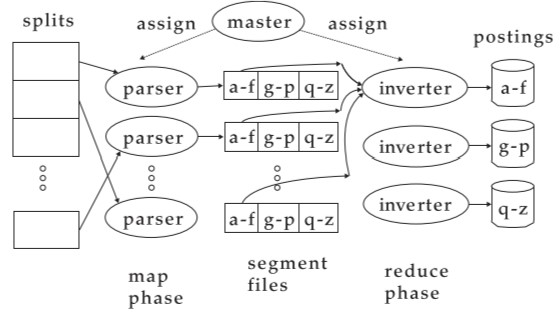
\includegraphics[scale = 1.5]{img/map reduce.jpg}
		\label{map reduce}
        \caption{MapReduce}
\end{figure}

\begin{enumerate}
    \item The input data (a collection of Web pages), is split into \textit{n splits}, where the size of each split is chosen so that the load is is distributed evenly and efficiently among the nodes. Usually, 16 or 64 MB are good choices;
    \item The splits are assigned to the nodes by the \textit{master node} on a ongoing basis: as a machine finishes processing one split, it is assigned to the next one;
    \item The \textit{map phase} consists of mapping splits to term-docID pairs, and since it is the same parsing in \textit{BSBI} and \textit{SPIMI}, we call the machines that execute the map phase \textbf{parsers}. Each parser writes its output to local intermediate files, called \textit{segment files};
    \item In the reduce phase, we would like to have all values for a given key to be stored close together, so that they can be read and processed quickly. This is achieved by \textbf{partitioning the keys} into $j$ term partitions and having the parsers write key-value pairs for each term partition into a separate segment file. In Picture \ref{map reduce}, the term partitions are according to first letter, and $j = 3$. Finally, each parser writes the corresponding segment file, one for each term partition, and each term partition thus corresponds to $r$ segment files, where $r$ is the number of parsers;
    \item The \textit{reduce phase} is performed by the \textbf{inverters}, which collect all values (docIDs) for a given key (termID) into one list. The master assigns each term partition to a different inverter and, as in the case of parsers, reassigns term partitions in case of failing or slow inverters. Each term partition (corresponding to $r$ segment files, one on each parser) is processed by one inverter;
    \item  Finally, the list of values is sorted for each key and written to the final sorted postings list (“postings” in the Picture).
\end{enumerate}

It is important to notice that parsers and inverters are not separate sets of machines, i.e. the same machine can be a parser in the map phase and an inverter in the reduce phase. In general, MapReduce offers a robust and conceptually simple framework for implementing index construction in a distributed environment. By providing a semiautomatic method for splitting index construction into smaller tasks, it can scale to almost arbitrarily large collections.

Picture \ref{map reduce example} shows an example of usage of MapReduce

\begin{figure}[h!]
		\centering
		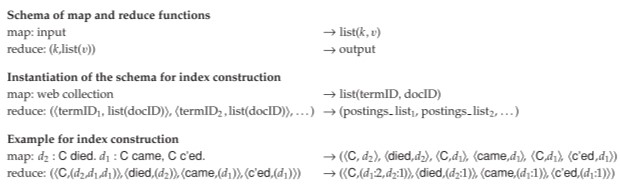
\includegraphics[scale = 1.5]{img/map reduce example.jpg}
		\label{map reduce example}
        \caption{Example of usage of MapReduce}
\end{figure}

\subsection{Dynamic indexing}
Thus far, we have assumed that the document collection is static, but most collections are modified frequently with documents being added, deleted, and updated. This means that new terms need to be added to the dictionary, and postings lists need to be updated for existing terms.

The simplest way to achieve this is to \textbf{periodically reconstruct the index} from scratch. This is a good solution if the number of changes over time is small and a delay in making new documents searchable is acceptable and if enough resources are available to construct a new index while the old one is still available for querying.

If there is a requirement that new documents be included quickly, one solution is to maintain two indexes: a \textit{large main index} and a \textit{small auxiliary index} that stores new documents. The auxiliary index is kept in memory, and the searches are run across both indexes and results merged. Deletions are stored in an invalidation bit vector, and we can then filter out deleted documents before returning the search result. Documents are updated by deleting and reinserting them. The main \textbf{issues} about this strategy may regard the merging phase: however, the merge of the auxiliary index into the main index could be efficient if we keep a separate file for each postings list. In this case, the merge operation would be the same as a simple append, but at the same time we would need to store a lot of files, which is inefficient for the OS. The simplest alternative, which is the one we assume for our purposes, is to store the index as one large file, i.e. a concatenation of postings lists; however, in reality a compromise between the two options is chosen.

Because of this complexity of dynamic indexing, some large search engines adopt a reconstruction-from-scratch strategy. They do not construct indexes dynamically. Instead, a new index is built from scratch periodically.

\subsection{Other types of indexes}

\begin{itemize}
    \item positional indexes;
    \item character n-gram indexes: as the text is parsed, the n-grams are enumerate. Then, for each n-gram we consider the pointers to all dictionary terms that contain it, i.e. the postings.
\end{itemize}

\section{Index Compression}\label{ch6}
In this chapter, we employ a number of compression techniques for dictionary and inverted index that are essential for efficient IR systems.

There are two more subtle \textbf{benefits} of compression:

\begin{enumerate}
    \item Increased use of \textbf{caching}: with compression, we can fit a lot more information into main memory. Instead of having to expend a disk seek when processing a query, we instead access its postings list in memory and decompress it. As we will see below, there are simple and efficient decompression methods, so that the penalty of having to decompress the postings list is small. As a result, we are able to \textbf{decrease the response time} of the IR system substantially;
    \item \textbf{Faster transfer of data from disk to memory}. Efficient decompression algorithms run so fast on modern hardware that the total time of transferring a compressed chunk of data from disk and then decompressing it is usually less than transferring the same chunk of data in uncompressed form.
\end{enumerate}

However, if the goal of compression is to conserve disk space and to decrease the response time of the IR system, then the \textbf{speed of the compression algorithm} itself is crucial: the compression algorithms we discuss in this chapter are highly efficient and can therefore serve all the purposes of index compression.

\underline{NOTE}: in this Chapter, we define a \textit{posting} as a docID in a postings list. For example, (6; 20, 45, 100), where 6 is the termID of the list's term, contains three postings.

\subsection{Statistical properties of terms in IR}
As in Chapter \ref{ch5}, we use \textit{Reuters-RCV1} as our model collection. We recall it main statistics in Picture \ref{reuters}, while in Picture \ref{statistics} we provide some terms and postings statistics of the collection.

\begin{figure}[h!]
		\centering
		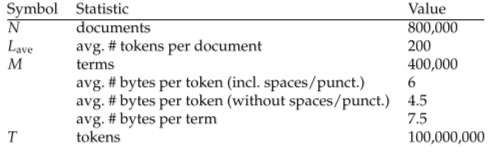
\includegraphics[scale = 1.5]{img/reuters.jpg}
		\label{reuters}
        \caption{Main statistics of \textit{Reuters-RCV1} collection}
\end{figure}

\begin{figure}[h!]
		\centering
		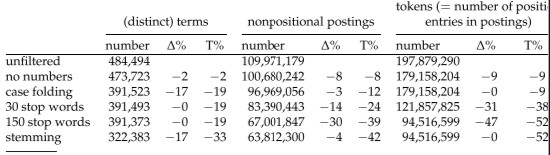
\includegraphics[scale = 1.7]{img/statistics.jpg}
		\label{statistics}
        \caption{Terms and postings statistics of \textit{Reuters-RCV1} collection}
\end{figure}

Some notes about these statistics follow:

\begin{itemize}
    \item the "$\Delta \%$" represents the reduction in size from the previous line;
    \item the "T\%" is the cumulative reduction from unfiltered;
    \item in general, the statistics show that \textbf{pre-processing} affects the size of the \textbf{dictionary} and the number of \textbf{non-positional postings} greatly: as we can see, stemming and case folding (i.e. considering "Rome" and "rome" as the same term) reduce the number of distinct terms by 17\%;
    \item the treatment of stopwords is also important: eliminating the 30 and 150 most common words from indexing cuts 31\% and 47\% of the total number of entries in postings, and 14\% and 30\% of the non-positonal postings;
    \item however, we notice that the usage of case folding and stemming does not change the number of entries in postings: this happens beacuse the positions of the terms are still kept in the postings;
    \item the same thing happens with the stopwords w.r.t. the number of distinct terms: we're only cutting off 30/150 words over a total of half million terms!
\end{itemize}

The compression techniques we describe in the remainder of this chapter are \textbf{lossless}, that is, \textbf{all information is preserved}. Better compression ratios can be achieved with \textbf{lossy} compression, which discards some information. Case folding, stemming, and stop word elimination are forms of lossy compression. In general, lossy compression makes sense when the “lost” information is unlikely ever to be used by the search system. For example, web search is characterized by a large number of documents, short queries, and users who only look at the first few pages of results. As a consequence, we can discard postings of documents that would only be used for hits far down the list. Thus, there are retrieval scenarios where lossy methods can be used for compression without any reduction in effectiveness.

Before introducing techniques for compressing the dictionary, we want to estimate the \textbf{number of distinct terms} (size of the vocabulary) $M$ in a collection. First of all, we notice that we cannot assume an upper bound; in practice, we will discover that the vocabulary size keep growing with the collection size.

\subsubsection{Heap's Law: estimating the number of terms}
The \textbf{Heap's Law} estimates the vocabulary size as a function of the collection size, in particular:

$$
M = kT^b
$$

, where:

\begin{itemize}
    \item $T$ is the number of tokens in the collection;
    \item $30 \leq k \leq 100$;
    \item $b \sim 0.5$.
\end{itemize}

The motivation of this law resides in the \textbf{linear relationship} between the collection size and the vocabulary size in a \textbf{log-log plot}, as represented in Picture \ref{heap}. 

\begin{figure}[h!]
		\centering
		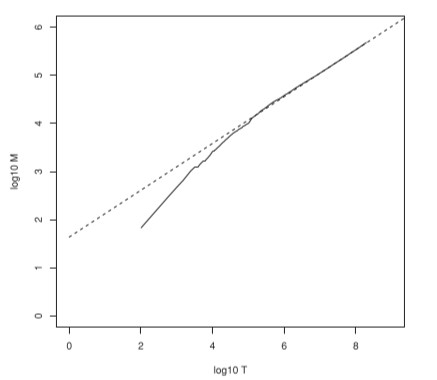
\includegraphics[scale = 1.7]{img/Heap law.jpg}
		\label{heap}
        \caption{Heap's Law: linear relationship between $M$ and $T$ in a log-log scale}
\end{figure}

As we can see, for RCV1 collection, the dashed line $\log_{10}M = 0.49 * \log_{10} T + 1.64$ represents the best least-square fit: in this case, $b = 0.49$ and $k = 44$. For example, for the first 1,000,020 tokens, Heap's Law predicts $44 * 1,000,020^{0.49} = 30,323$ terms, while the dashed line predicts 38,365 terms, so it is a good approximation.

Notice that the parameter $k$ is quite variable because vocabulary growth depends a lot on the nature of the collection and how it is processed. Case-folding and stemming reduce the growth rate of the vocabulary, whereas including numbers and spelling errors increase it.

In general, regardless of the values of the parameters for a particular collection, Heaps’ law suggests that:

\begin{enumerate}
    \item The dictionary size continues to increase with more documents in the collection, rather than a maximum vocabulary size being reached;
    \item The size of the dictionary is quite large for large collections
\end{enumerate}

These two hypotheses have been empirically shown to be true of large text collections, so dictionary compression is a crucial operation for an effective IR system.

\underline{Exercise}: Compute the vocabulary size for this scenario. There are 3,000 different terms ($M_1$) in the first 10,000 tokens ($T_1$), and 30,000 different terms ($M_2$) in the first 1,000,000 tokens($T_2$). Assume a search engine indexes a total of 20,000,000,000 (= $2^{10}$) pages, each containing 200 tokens on average. What is the size of the vocabulary of the indexed collection as predicted by the Heap's Law? 

\subsubsection{Zipf's Law}
While Heap's Law gives the vocabulary size, \textbf{Zipf's Law} helps us understanding how the terms are distributed across documents, so it takes into account the relative frequencies of terms, as we know that in natural languages, there are a few very frequent terms and very many rare terms.

If we assume that the terms are ranked from the most frequent to the least frequent, we can consider:
\begin{itemize}
    \item $t_i$ to be the term at rank $i$ in the collection;
    \item $cf_i$ to be the collection frequency, i.e. the number of occurrences of the term $t_i$, i.e. the term at rank $i$, in the collection;
    \item $df_i$ to be the document frequency, i.e. the total number of documents that contain the term $t_i$ in the corpus;
    \item $tf_{i,d}$ to be the term frequency, i.e. the total number of occurrences of the term in a document
\end{itemize}

Zipf's Law states that if $t_1$ is the most common term in the collection, $t_2$ is the next most common, and so on, then the collection frequency $cf_i$ of the i-th
most common term is proportional to $1/i$, i.e.:

$$
cf_i \propto \frac{1}{i}
$$

In this sense, if the most frequent term occurs $cf_i$ times, then the second most common will occur half of the occurrences, and the third one third of the occurrences and so on.. Another way of stating Zipf's Law is:

$$
cf_i = ci^{-1}
$$

or

$$
\log cf_i = \log c  - \log i
$$

, where $c$ is a constant. As we can see, there is a linear relationship between $\log cf_i$ and $\log i$, with slope -1, as represented in Picture \ref{zip}.

\begin{figure}[h!]
		\centering
		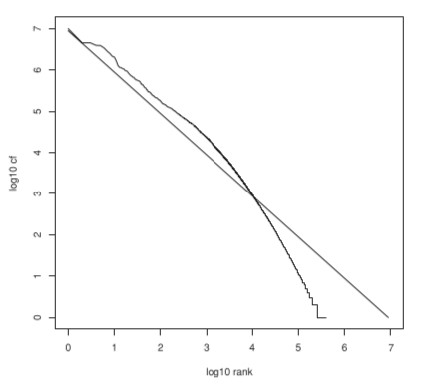
\includegraphics[scale = 1.7]{img/zipf law.jpg}
		\label{zip}
        \caption{Zipf's Law: linear relationship between $cf_i$ and $i$ in a log-log scale}
\end{figure}

Moreover, if we consider the relationship $cf_i = ci^{-1}$, we can recognize a \textbf{Power Law relationship}: the Power Law states that $p(i) \approx k i^{-\alpha}$, i.e. that roughly 80\% of the total popularity comes from 20\% of the terms. Notice that the quantity $\alpha$ represents the slope in the log-log plot of $p$ and $i$.

\subsection{Dictionary compression}
This section presents a series of dictionary data structures that achieve increasingly higher compression ratios. The main reason for compressing the dictionary is to fit it in memory, in order to reduce the number of disk accesses when processing a query. Indeed, some embedded/small devices may have very little memory. 

\subsubsection{Dictionary as a string}
The simplest data structure for the dictionary is to sort the vocabulary lexicographically and store it in an \textbf{array of fixed-width entries} as shown in Picture \ref{dic string}.

\begin{figure}[h!]
		\centering
		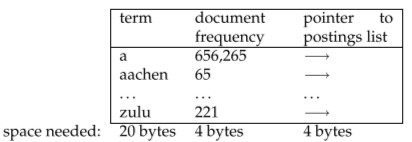
\includegraphics[scale = 1.7]{img/dictionary string.jpg}
		\label{dic string}
        \caption{Dictionary as an array of fixed-width entries}
\end{figure}

If we allocate 20 bytes for the term itself, 4 bytes for its document frequency and 4 bytes for its pointer to its postings list, then for Reuters-RCV1 we need 400,000 x 28 = 11.2 MB for storing the dictionary. Notice that the lexicographical order allows us to perform a binary search for looking up terms. However, using fixed-width entries for terms is clearly wasteful, since the average length of a term in English is about eight characters, so on average we are wasting twelve characters. Also, we have no way of storing terms with more than twenty characters. 

We can overcome these issues by storing the dictionary terms as one \textbf{long string of characters}, as shown in Picture \ref{dic string 2}.

\begin{figure}[h!]
		\centering
		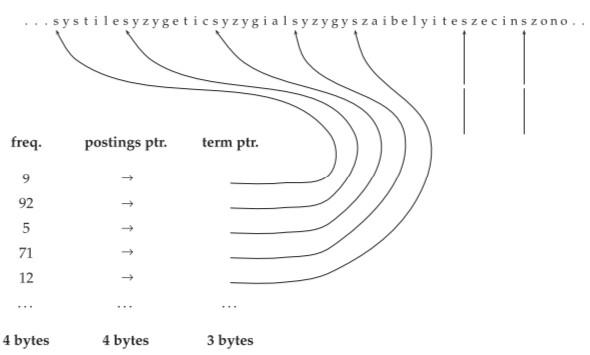
\includegraphics[scale = 1.7]{img/dictionary string_2.jpg}
		\label{dic string 2}
        \caption{Dictionary as a string}
\end{figure}

In this case, for each term we use 4 bytes for storing the term frequency, 4 bytes for storing the pointer to the corresponding postings list, 3 bytes for storing the term pointer and an average of 8 bytes for storing the term in the string. In this way, we only use an average of 11 bytes per term, versus the 20 bytes we used before, resulting in a 60\% storage save. In this case, we have a total of 19 bytes, so 400,000 x 19 = 7.6 MB, against the 11.2 MB used in the fixed-width entries. Notice that, as before, the look for a term can be done by performing a binary search operation, and that in this case the end of the string is not stored, since the term pointer of the next term is used as indicator of the end of the current term.

\subsubsection{Blocked storage}
We can further compress the dictionary by grouping terms in the string into blocks of size $k$ and keeping a term pointer only for the first term of each block, as represented in Picture \ref{blocked}.

\begin{figure}[h!]
		\centering
		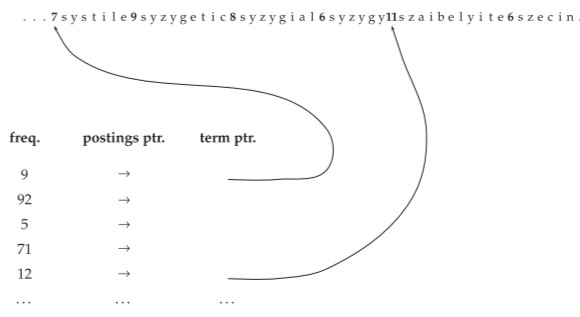
\includegraphics[scale = 1.7]{img/blocked storage.jpg}
		\label{blocked}
        \caption{Blocked storage}
\end{figure}

In this case we store the length of the term in the string as an additional byte at the beginning of the term: we thus eliminate $(k-1)$ term pointers, but need an additional $k$ bytes for storing the length of each term. If $k = 4$ we save $(k-1)$ x 3 = 9 bytes for term pointers, but we need an additional $k = 4$ bytes for term lengths. In the case of Reuters-RCV1, we reduce 5 bytes per four-term block, resulting in a total of 0.5 MB, bringing us down to 7.1 MB.

By increasing the block size k, we get better compression. However, there is a \textbf{tradeoff} between \textbf{compression} and the \textbf{speed of term lookup}. Suppose we have an eight-term dictionary, as represented in Picture \ref{example}.

\begin{figure}[h!]
		\centering
		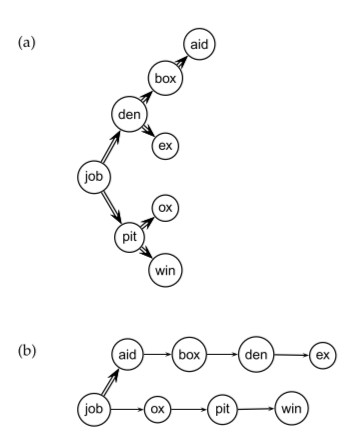
\includegraphics[scale = 1.7]{img/example .jpg}
		\label{example}
        % \caption{Search on uncompressed and compressed dictionary}
\end{figure}

In the Picture, steps in binary search are showed as double lines, and steps in list search as simple lines. We search for terms in the uncompressed dictionary by binary search (a). In the compressed dictionary, we first locate the term’s block by binary search and then its position within the list by linear search through the block (b). Searching the uncompressed dictionary in (a) takes on average (0 + 1 + 2 + 3 + 2 + 1 + 2 + 2)/8, i.e. more or less 1.6 steps, assuming each term is equally likely to come up in a query. For example, finding the two terms, \textit{aid} and \textit{box}, takes three and two steps, respectively. With blocks of size k = 4 in (b), we need (0+1+2+3+4+1+2+3)/8 = 2 steps on average, i.e. 25\% more. By increasing k, we can get the size of the compressed dictionary arbitrarily close to the minimum of 400,000 × (4 + 4 + 1 + 8) = 6.8 MB, but term lookup becomes prohibitively slow for large values of k.

However, by now we did not exploit the redundancy in the dictionary, in particular the fact that consecutive entries in an alphabetically sorted list share common prefixes. The exploitation of this property leads to \textit{front coding}.

\begin{figure}[h!]
		\centering
		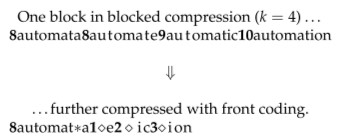
\includegraphics[scale = 2.0]{img/front coding.jpg}
		\label{front}
        \caption{Front coding: first implementation}
\end{figure}

In this case, a \textbf{common prefix} is identified for a sub-sequence of the term list, and then referred to with a special character. As we can see, the compression with front coding includes the common prefix, and each of the following characters for each term in the uncompressed sub-sequence. Together with the characters, the extra length beyond the suffix is stored, leading to a much smaller representation. In the case of Reuters-RCV1, this strategy saves another 1.2 MB. However, this is not the only possible implementation of the idea of front coding: Picture \ref{front2} show another implementation in which each term exploits a prefix of the previous one.

\begin{figure}[h!]
		\centering
		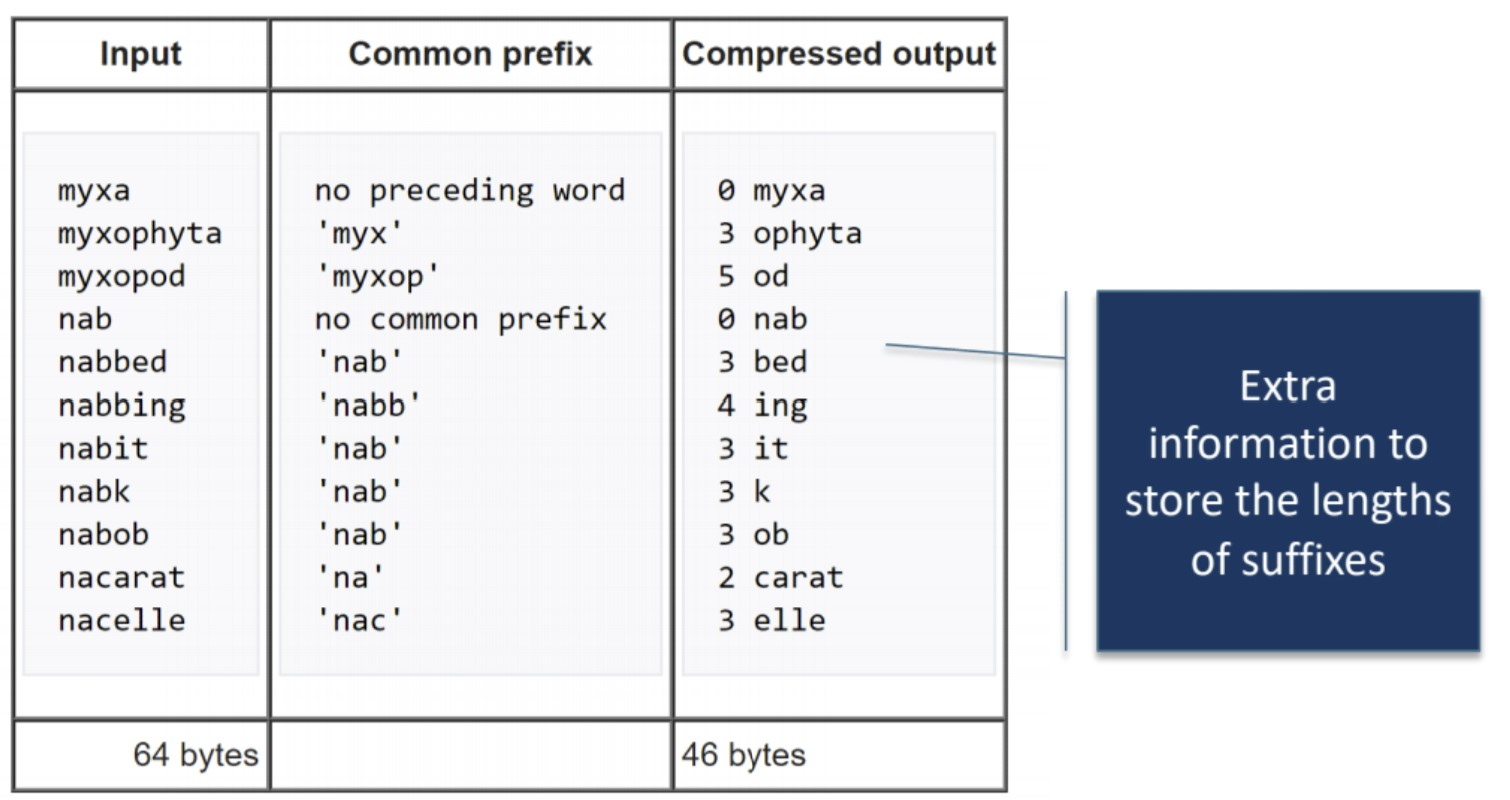
\includegraphics[scale = 0.5]{img/front coding2.jpg}
		\label{front2}
        \caption{Front coding: second implementation}
\end{figure}

However, even with the best compression scheme, it may not be feasible to store the entire dictionary in main memory for very large text collections and for hardware with limited memory. Picture \ref{summary} provides a summary of the dictionary compression achieved using the data structures we described so far.

\begin{figure}[h!]
		\centering
		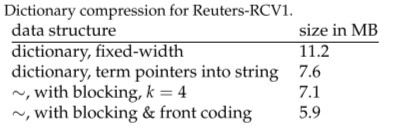
\includegraphics[scale = 2.0]{img/summary compression.jpg}
		\label{summary}
        \caption{Dictionary compression: summary}
\end{figure}

\subsection{Postings compression}
We recall the statistics of Reuters-RCV1 collection: as we can see, the number of postings, i.e. the number of docIDs in a postings list, is 100,000,000. DocIDs are $\log_{2}800,000 \approx 20$ bits long, so the size of the collection is 800,00 x 200 x 6 bytes = 960 MB, while the size of the uncompressed postings file is 100,000,000 x 20/8 = 150 MB.

\begin{figure}[h!]
		\centering
		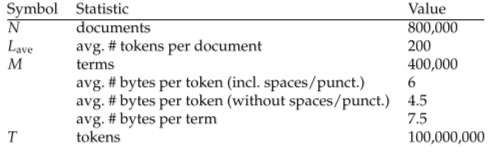
\includegraphics[scale = 1.5]{img/reuters.jpg}
		\label{reuters}
        \caption{Main statistics of \textit{Reuters-RCV1} collection}
\end{figure}

To use a more efficient representation of the postings file, i.e. a representation that uses less than 20 bits per document, we can exploit the fact that postings for frequent terms are close together. As represented in Picture \ref{gaps}, a very \textbf{frequent term} will have postings whose \textbf{gaps} are very \textbf{close}, and for which much less than 20 bits can be used, so in this case the idea is to store the gaps instead of the docIDs; on the other hand, gaps for a \textbf{rare term} have the \textbf{same order of magnitude as the docIDs}, so they need 20 bits. In this sense, we need a \textit{variable encoding} method that uses fewer bits for smaller gaps.

\begin{figure}[h!]
		\centering
		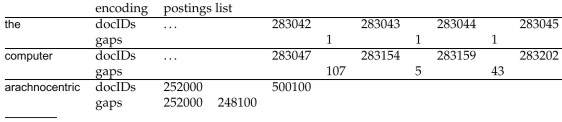
\includegraphics[scale = 2.0]{img/gaps.jpg}
		\label{gaps}
        \caption{Encoding gaps}
\end{figure}

To encode small numbers in less space than large numbers, we look at two types of methods: \textbf{bytewise compression} and \textbf{bitwise compression}. As the names suggest, these methods attempt to encode gaps with the minimum number of bytes and bits, respectively.

\subsubsection{Variable byte encoding}
Variable byte (VB) encoding uses an integral number of bytes to encode a gap $G$:

\begin{itemize}
    \item the last 7 bits of a byte are \textit{payload} and encode part of the gap;
    \item the first bit of the byte is a \textit{continuation bit}: it is set to 1 for the last byte of the encoded gap and to 0 otherwise.
\end{itemize}

To decode a variable byte code, we read a sequence of bytes with continuation bit 0 terminated by a byte with continuation bit 1. We then extract and concatenate the 7-bit parts. An example of VB-encoded postings list is provided in Picture \ref{vb}.

\begin{figure}[h!]
		\centering
		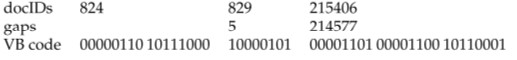
\includegraphics[scale = 2.0]{img/VB encoding.jpg}
		\label{vb}
        \caption{Example of VB encoding}
\end{figure}

A key property of VB encoding is that VB-encoded postings are \textbf{uniquely prefix-decodable}, i.e. no whole code word in the system is a prefix of any other code word. This means that no special marker is needed to separate codes.

With VB compression, the size of the compressed index for Reuters-RCV1 is 116 MB as we verified in an experiment: this is a more than 50\% reduction of the size of the uncompressed index. 

The idea of VB encoding can also be applied to larger or smaller units than bytes: 32-bit words, 16-bit words, and 4-bit words or nibbles. \textbf{Larger words} further \textbf{decrease} the \textbf{amount of bit manipulation} necessary at the cost of less effective (or no) compression. In general, \textbf{bytes} offer a \textbf{good compromise} between \textbf{compression ratio} and \textbf{speed of decompression}, and for most IR systems \textbf{variable byte codes} offer an excellent \textbf{tradeoff} between \textbf{time} and \textbf{space}, and they are also simple to implement. However, if the disk space is a scarce resource, we can achieve better compression ratios by using bit-level encodings, in particular two closely related encodings: $\gamma$ codes, which we will turn to next, and $\delta$ codes.

\subsubsection{Elias-$\gamma$ encoding}
While VB codes use a variable number of bytes for encoding a gap, bit-level codes use a finer grained bit level. The simplest bit-level code is the \textbf{unary code}, which represents $n$ as a string of $n$ 1's followed by a 0, as showed in the first column of Picture \ref{gamma}.

\begin{figure}[h!]
		\centering
		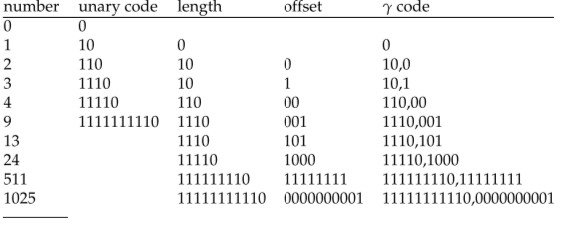
\includegraphics[scale = 2.0]{img/gamma encoding.jpg}
		\label{gamma}
        \caption{Examples of unary and $\gamma$ codes}
\end{figure}

Clearly, the unary code is not efficient, but it will become handy later.

In general, how efficient can a code be in principle? Assuming the $2^n$ gaps $G$ with $1 \leq G \leq 2^n$ are all equally likely, the optimal encoding uses $n$ bits for each $G$. So some gaps cannot be encoded with fewer than $\log_2 G$ bits. Our goal is to get as close to this lower bound as possible.

A method that is within a factor of optimal is $\gamma$ encoding. $\gamma$ codes implement \textbf{variable-length encoding} by \textbf{splitting} the representation of a gap $G$ into a pair of \textbf{length} and \textbf{offset}:

\begin{itemize}
    \item the \textit{offset} is $G$ in binary, but with the leading 1 removed. For example, for 13 (binary 1101), the \textit{offset} is 101;
    \item the \textit{length} encodes the length of \textit{offset} in unary code. For 13, the length of \textit{offset} is 3 bits, which is 1110 in unary.
\end{itemize}

The $\gamma$ code is then the \textbf{concatenation} of \textit{length} and \textit{offset} (in the example, the $\gamma$ code of 13 is therefore 1110101). Picture \ref{gamma} provides some other examples. The \textbf{encoding} of a $\gamma$ code works as follows:

\begin{enumerate}
    \item Read the unary code up to the 0 that terminates it, for example the four bits 1110 when decoding 1110101. Now we know that the offset is long 3 bits;
    \item The offset is read correctly, and the 1 is preprended, leading to 1101 = 13.
\end{enumerate}

In general:

\begin{itemize}
    \item the length of the \textit{offset} is $\lfloor \log_2 G \rfloor$ bits;
    \item the length of the \textit{length} is $\lfloor \log_2 G \rfloor + 1$
\end{itemize}

so the length of the entire code is $2 \lfloor \log_2 G \rfloor + 1$ bits. 

All the $\gamma$ codes have an odd number of bits, and they are within a factor of 2 of the optimal encoding $\log_2 G$ for any distribution, which makes the $\gamma$ codes to be \textbf{universal}. In addition to universality, $\gamma$ codes are \textbf{prefix free}, i.e. no $\gamma$ code can be the prefix of another, meaning that there is always a unique decoding of a sequence of $\gamma$ codes. The other property is that $\gamma$ codes are \textbf{parameter free}, which simplifies the implementation and the decompression of this code. However, a \textbf{disadvantage} of this encoding is that it is relatively inefficient for large numbers, since the unary code is used for encoding the offset.

The result of running $\gamma$ compression on Reuters-RCV1 is that the size of the compressed index is 101 MB, which is less than VB encoding.

Picture \ref{summary with post} shows a summary of the results of the compression techniques we exploited thus far.

\begin{figure}[h!]
		\centering
		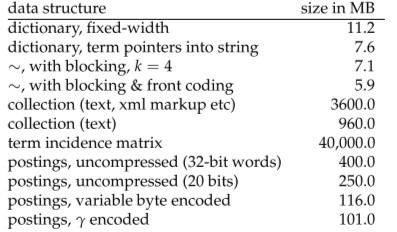
\includegraphics[scale = 2.0]{img/summary with postings.jpg}
		\label{summary with post}
        \caption{Summary of compression techniques including postings}
\end{figure}

\subsubsection{Elias-$\delta$ encoding}
A slight variation of the $\gamma$ codes are the $\delta$, in which again the gap $G$ is represented into a pair of \textit{length} and \textit{offset}:

\begin{itemize}
    \item the \textit{offset} is $G$ in binary, but with the leading 1 removed. For example, for 13 (binary 1101), the \textit{offset} is 101. It is the same as $\gamma$ codes;
    \item the \textit{length} encodes the length of \textit{offset} in $\gamma$ code.
\end{itemize}

In this case, $\delta$ encoding uses $2 \lfloor \log_2 \lfloor \log_2 G \rfloor \rfloor + 1$ bits.

\subsubsection{Golomb-Rice encoding}
Golomb-Rice encoding works as follows: we choose a quantity $M = 2^j$, where $j$ is a parameter of the method, and we encode an integer $n$ by splitting $n$ into two components, the quotient $q(n)$ and the remainder $r(n)$, where:

\begin{itemize}
    \item $q(n) = \lfloor \frac{n-1}{M} \rfloor$;
    \item $r(n) = (n-1) mod M$, i.e. $0 \leq r(n) \leq M - 1$.
\end{itemize}

Then, $n$ is encoded by writing $q(n) + 1$ in unary, followed by $r(n)$ as a binary number represented on $\log_2 M$ (= $j$) bits. In general, $j$ is chosen so that $2^j$ is centered around the mean of the elements to be represented.

\subsubsection{Interpolative coding}
A completely different approach is taken by the binary interpolative coding, which directly encodes strictly monotone sequences, and in particular this method recursively splits the sequence in two halves: the element in the middle is encoded, then the recursion is applied in the two halves.

We consider an example: suppose we have the following inverted list: <7; 3, 8, 9, 11, 12, 13, 17> in a collection of $N$ = 20 documents. Suppose that the value of the second pointer is somehow known before the first must be coded. In the example, if it is known that the second pointer is to document 8, then the first pointer is restricted to some document number in the range 1 to 7 inclusive. A simple assignment of binary codewords then suffices to represent this first document pointer in three bits. Suppose now that the fourth as well as the second document number is known. The fourth document pointer is to document 11, so the third pointer is constrained to the range 9 to 10. Again, a simple code (in this case just one bit long) can be used to represent the third pointer. The brevity of this codeword is a direct consequence of the fact that there is a cluster and that both the upper and lower bounding pointers are also in the cluster. As an even more extreme example, if both the fourth and the sixth pointers are known (to documents 11 and 13, respectively), then the fifth document pointer can be represented using a codeword zero bits long, since it must be to document 12.

This representation is based upon the supposition that the second, fourth, and sixth pointers are known. To represent them, a list <3; 8,11,13> must have been previously coded. The same technique can be used for this list too. If the second pointer (to document 11) is known, then the first pointer (to document 8) takes at most four bits. Indeed, since there must be a pointer to the left and a pointer to the right of this document, the range can be further narrowed to 2 .. . 9 inclusive, and a three-bit code can be used. By a similar argument, the third pointer must lie between 13 = 12 + 1 and 19 = 20 — 1 inclusive, and 3 - $\lfloor \log 7 \rfloor$ bits suffice.

It is possible to show that at its worst the interpolative code is only slightly inefficient compared with a Golomb code, and, because contiguous sets of values can be coded in less than one bit each, at its best it can be dramatically better. Moreover, in practice the interpolative code usually results in very good compression. Indeed, the only real drawback of the method is its complexity of implementation—encoding and each decoding make use of a stack of pending values, and the encoding and decoding loops become rather more detailed than for the simpler Golomb and $\gamma$ codes.

\subsubsection{Information theory}
Shannon showed that if we know that a random variable $X$ takes values with a discrete probability distribution $P = p_1, .., p_n$, then the minimum expected message length we can achieve with any binary prefix-free code is between $H(P)$ and $H(P) + 1$, where $H(P)$ is the \textbf{entropy}, which is defined as:

$$
H(P) = \sum_i p_i \log \frac{1}{p_i}
$$

For example, Elias-$\gamma$ encoding is optimal when the integers to be compressed conform the following probability distribution: $P(n) = \frac{1}{2n^2}$, i.e. the probability of small numbers is very high, or, in other terms, the probability of the numbers is inversely proportional to the magnitudes of the gaps.

Huffman encoding is known to be \textbf{optimal} w.r.t. the Shannon theory: in particular, this encoding is based on the entropy, and its goal is to represent more common symbols using fewer bits than less common ones. This encoding works for every possible probability distribution of integers, but its drawback is that it requires traversing a tree or performing slow table lookups.

\section{Scoring, term weighting and the vector space model}\label{ch7}

\subsection{Ranked retrieval}
Thus far, we've only considered Boolean queries, and in this sense, either a document satisfies a query or not. This methodology is good for expert users with precise understanding of their needs and the collection, but it is not good for most of the users, who are not capable of writing Boolean queries. Another problem of Boolean queries is the so-called \textit{feast or famine} problem, i.e. Boolean queries often result in either too few or too many results.

For these reasons, rather then retrieving a set of documents satisfying a query expression, in \textbf{ranked retrieval} the system reorders the top documents of a collection w.r.t. a given query. In this case, rather than a query language consisting in operators and expressions, the system deals with \textbf{free text queries}, i.e. a collection of words in human language. Notice that in the case of \textit{ranked retrieval}, the  \textit{feast or famine} issue is no longer a problem, since we just provide the top-$k$ results. 

\subsection{Parametric and zone indexes}
We have thus far viewed a document as a sequence of terms. In fact, most documents have \textbf{additional structure}. Digital documents generally encode, in machine-recognizable form, certain \textbf{metadata} associated with each document, such as its author(s), title and date of publication etc.. This metadata would generally include \textit{fields} such as the date of creation and the format of the document, as well the author and possibly the title of the document. The possible values of a field should be thought of as finite (for instance, the set of all dates of authorship). 

Consider queries of the form “find documents authored by William Shakespeare in 1601, containing the phrase \textit{alas poor Yorick}”. Query processing then consists as usual of postings intersections, except that we may merge \textbf{postings} from standard inverted as well as \textbf{parametric indexes}. There is \textbf{one} parametric index \textbf{for each field}, and it allows us to select only the documents matching a date specified in the query (in the example query above, the year 1601 is one such field value). The search engine may support querying ranges on such ordered values; to this end, a structure like a \textit{B-tree} may be used for the field’s dictionary. 

\textit{Zones} are similar to \textit{fields}, except the \textbf{contents} of a zone can be \textbf{arbitrary free text}, while a field may take on a relatively small set of values. For instance, document titles and abstracts are generally treated as zones. We may build a separate \textbf{inverted index for each zone of a document}, to support queries such as “find documents with \textit{merchant} in the title and \textit{william} in the author list and the phrase \textit{gentle rain in the body}”. This has the effect of building an index that looks like Picture \ref{zi}.

\begin{figure}[h!]
		\centering
		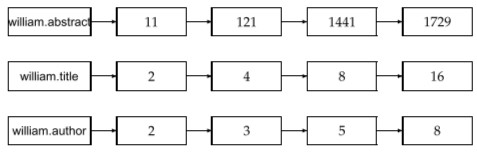
\includegraphics[scale = 2.0]{img/zone index.jpg}
		\label{zi}
        \caption{Basic zone index}
\end{figure}

We can reduce the size of the dictionary by encoding the zone in which a term occurs in the postings. In Picture \ref{zip} for instance, we show how occurrences of \textit{william} in the title and author zones of various documents are encoded. Such an encoding is useful when the size of the dictionary is a concern (because we require the dictionary to fit in main memory). 

\begin{figure}[h!]
		\centering
		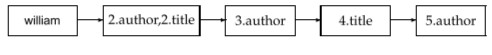
\includegraphics[scale = 2.0]{img/zone index with postings.jpg}
		\label{zip}
        \caption{Zone index in which the zone is encoded in the postings rather than the dictionary}
\end{figure}

But there is another important reason why the encoding of Figure \ref{zip} is useful: the efficient computation of scores using a technique we will call weighted zone.

\subsection{Term frequency and weighting}
Obviously, the core of the \textit{ranked retrieval} approach relies on the way we provide the \textbf{score} to each of the document, and in particular on the way we measure the importance of a query term w.r.t. the documents in the collection. 

One approach could be represented by considering the \textbf{Jaccard} coefficient between the vectors representing the query and the document. For example, if the query is "\textit{ides of march}", and the first document is "\textit{caesar died in march}" and the second document is "\textit{the long march}", then the Jaccard coefficients are:

$$
J(q,d_1) = \frac{1}{3+4-1} = \frac{1}{6}
$$

and 

$$
J(q,d_2) = \frac{1}{3+3-1} = \frac{1}{5}
$$

In this way, the result is that the second document is more relevant than the first one, but this is clearly not the case: clearly the Jaccard coefficient does not consider the \textit{term frequency}, i.e. the number of times a term occurs in a query.

Another approach is to assign the weight to be equal to the \textbf{number of occurrences} of term $t$ in document $d$. This weighting scheme is referred to as \textbf{term frequency} and is denoted $tf(t,d)$. Notice that for a document $d$, the set of weights determined by the \textit{term frequency} does not depend on the order of the terms in the document, since we only focus on the information about the number of occurrences of each term. This model is often called as \textit{bag of words} models. 

\subsubsection{Log-frequency and inverse document frequency}
Clearly, this raw definition of term frequency is not what we want from the IR system to be implemented: a document $d_1$ with 10 occurrences of a term is more relevant than a document $d_2$ with only 1 occurrence of a term, but $d_1$ is not 10 times more relevant than $d_2$. In other words, we do not want the relevance of a term to be directly proportional to its frequency.

One possible solution could be of considering the \textbf{log-frequency}, i.e.:

$$
\log tf(t,d) = \begin{cases}
1 + \log_{10} tf(t,d) \quad \text{if }tf(t,d)>0\\
0 \quad \text{otherwise }
\end{cases}
$$

In this way, the score of a query-document pair is defined as:

$$
\text{score}_{\text{LOG}}(q,d) = \sum_{t \in q \cap d} (1 + \log tf(t,d))
$$

Another possible solution exploits the \textbf{document frequency} concept: the \textit{document frequency} of a term $t$ represents the number of documents in the collection that contain the term $t$. The idea when considering \textit{document frequency} is that rare terms are more informative than frequent terms, so the documents that contain these rare terms are more likely to be relevant than documents that do not. In this sense, the \textit{document frequency} is an \textbf{inverse measure} of the \textbf{informativeness} of a term $t$. Notice that, for each term $t$, $df(t) \leq N$, where $N$ is the number of documents in the collection. The way the \textit{document frequency} is used for measuring the relevance of a term $t$ is represented by the \textbf{inverse document frequency}, which is defined as:

$$
idf(t) = \log_{10}(\frac{N}{df(t)})
$$

Some notes:

\begin{itemize}
    \item the $\log_{10}$ is used as a smoothing factor for the effect of $idf$;
    \item very frequent terms have small values of $idf$;
    \item rare terms have large values of $idf$.
\end{itemize}

In this case, the score of a query-document pair is defined as:

$$
\text{score}_{\text{IDF}}(q,d) = \sum_{t \in q \cap d} idf(t) = \sum_{t \in q \cap d} \log_{10}(\frac{N}{df(t)})
$$

Notice that $idf$ alone can produce a ranking of the matching documents only for queries with at least two terms, if all the docs do not contain all query terms.

\subsubsection{tf-idf}
We now combine the definitions of term frequency and inverse document frequency, to produce a composite weight for each term in each document, the \textit{tf-idf}:

$$
\textit{tf-idf}(t,d) = tf(t,d) * idf(t)
$$

Notice that:

\begin{itemize}
    \item the weight is higher for a term that appears many times within a small number of documents;
    \item the weight is lower for a term that occurs fewer times in a document, or that occurs in many documents. The lowest weight is obtained when the term occurs in all the documents.
\end{itemize}

At this point, we may view each document as a vector with one component corresponding to each term in the dictionary, together with a weight for each component that is given by the \textit{tf-idf}; in this case, we can compute the score as:

$$
\text{score}_{\text{TF-IDF}}(q,d) = \sum_{t \in q \cap d} \textit{tf-idf}(t,d)
$$

\underline{Example}: if we consider the table of term frequencies and idf values of Picture  \ref{ex} ,the score of Doc 1 is given by:

\begin{figure}[h!]
		\centering
		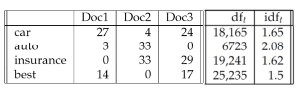
\includegraphics[scale = 2.0]{img/example tf idf.jpg}
		\label{ex}
        %\caption{Summary of compression techniques including postings}
\end{figure}

\begin{itemize}
    \item \textit{car} = $27 * 1.65 = 44.55$;
    \item \textit{insurance} = $0$;
    \item \textit{auto} = $3* 2.08 = 6.24$;
    \item \textit{best} = $14 * 1.5 = 21$
\end{itemize}

\subsection{Vector space model for scoring}
Thus far we developed the notion of a document vector that captures the relative importance of the terms in a document. The representation of a set of documents as vectors in a common vector space is known as the \textbf{vector space model} and is fundamental to a host of information retrieval operations ranging from scoring documents on a query, document classification and document clustering. The peculiarities of the documents as vectors are:

\begin{itemize}
    \item They're very \textbf{high-dimensional vectors}, i.e. they belong to an high-dimension vector space;
    \item They are very \textbf{sparse vectors}, i.e. most of the entries are equal to 0.
\end{itemize}

We recall that the goal of \textit{ranked retrieval} is to rank the documents of the collection according to their proximity to a given query. In this sense, we must provide both the vector representation for queries and the definition of proximity/similarity between vectors.

\subsubsection{Vector similarity}
We first deal with the concept of vector similarity, and we start our reasoning by considering the \textbf{euclidean distance} between two vectors. Given a document $d$ and a query $q$, the euclidean distance is defined as:

$$
dist_{\text{EUCLIDEAN}}(d,q) = \sqrt{\sum_{i = 1}^n (d_i - q_i)^2}
$$

, where $n$ is the dimensionality of the vectors. In general, the Euclidean distance is not a good measure of similarity, since it assumes large values for vectors of different lengths, i.e. the Euclidean distance of two close vectors can be very high due to their length, as represented in Picture \ref{eucl}. As we can see, the value of the Euclidean distance of $q$ and $d_2$ is very high, even if the distribution of their terms is quite similar.

\begin{figure}[h!]
		\centering
		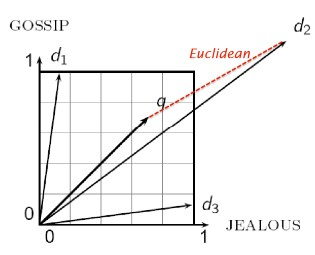
\includegraphics[scale = 2.0]{img/eucl.jpg}
		\label{eucl}
        \caption{Example of Euclidean distance}
\end{figure}

Another possible measure of the similarity of two vectors could rely on the \textbf{angle} between the vectors. In this sense, we could rank documents in increasing order of \textbf{cosine similarity} w.r.t. the query:

$$
sim_{\text{COSINE}}(\Vec{q},\Vec{d}) = \frac{\Vec{q} \cdot \Vec{d}}{|\Vec{q}||\Vec{d}|} = \frac{\sum_i q_i d_i}{\sqrt{\sum_i q_i^2} \sqrt{\sum_i d_i^2}} = \cos{\theta}
$$

, where:

\begin{itemize}
    \item $\Vec{q} \cdot \Vec{d}$ represents the \textit{dot product} between $q$ and $d$;
    \item $|\Vec{q}|$ and $|\Vec{d}|$ are the \textit{Euclidean lengths} of $\Vec{q}$ and $\Vec{d}$, and they're used to normalize the vectors $\Vec{q}$ and $\Vec{d}$ to unit vectors $\Vec{q} / |\Vec{q}|$ and $\Vec{d} / |\Vec{d}|$. In this way, long and short documents have now comparable weights.
\end{itemize}

Notice that the definition of $sim_{\text{COSINE}}$ is equal to the cosine of the angle $\theta$ between the two vectors, as showed in Picture \ref{cosine}.

\begin{figure}[h!]
		\centering
		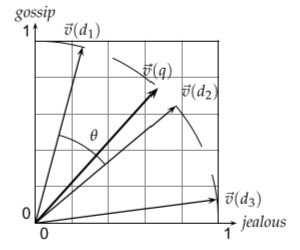
\includegraphics[scale = 2.0]{img/cosine.jpg}
		\label{cosine}
        \caption{Example of cosine similarity}
\end{figure}

What is the usage of cosine similarity?  Given a document $d$ (potentially one of the $d_i$ in the collection), consider searching for the documents in the collection most similar to $d$: we reduce the problem of finding the document(s) most similar to $d$ to that of finding the $d_i$ with the highest dot products $\Vec{d} \cdot \Vec{d_i}$. We could do this by computing the dot products between $\Vec{d}$ and each of $\Vec{d_1},..,\Vec{d_n}$, then picking off the highest resulting values.

\underline{Example}: Picture \ref{example cosine} represents the term frequencies for 4 terms in 3 different novels: in this sense, each of the novels is represented as a unit vector in three dimensions, resulting in the term frequencies weights of Picture \ref{example cosine}.

\begin{figure}[h!]
		\centering
		\includegraphics[scale = 2.0]{img/example cosine 1.jpg}
        \includegraphics[scale = 2.0]{img/example cosine 2.jpg}
		\label{example cosine}
        %\caption{Example of cosine similarity}
\end{figure}

In this case, $sim_{\text{COSINE}}(\Vec{SaS}, \Vec{PaP}) = 0.996 * 0.993 + 0.087 * 0.120 + 0.017 * 0 = 0.999 $ 

Viewing a collection of $N$ documents as a collection of vectors leads to a natural view of a collection as a term-document matrix: this is an $M \times N$ matrix whose rows represent the $M$ terms of the $N$ columns, each of which corresponds to a document. As always, the terms being indexed could be stemmed before indexing;

\subsubsection{Queries as vectors}
After discussing the concept of vectors similarity, we can now notice that we can also view a query as a vector. In this way, we can assign to each document $d$ a score equal to the dot product:

$$
\text{score} = \Vec{q} \cdot \Vec{d}
$$

In other words, we can consider a query as a very short document, so we can use the cosine similarity between the query vector and a documents vector as a measure of the score of the document for that query:

$$
\text{score} = sim_{\text{COSINE}(\Vec{q}, \Vec{d})} = \frac{\Vec{q} \cdot \Vec{d}}{|\Vec{q}||\Vec{d}|}
$$

Finally, the resulting scores can be used to select the top-scoring documents for a query. However, computing the cosine similarities between the query vector and each document vector in the collection, sorting the resulting scores and selecting the top-K documents can be expensive, since a single similarity computation can entail a dot product in tens of thousands of dimensions, demanding many arithmetic operations.

\subsubsection{Computing vector scores}
In a typical setting we have a collection of documents each represented by a vector, a free text query represented by a vector, and a positive integer K: we seek the K documents of the collection with the highest vector space scores on the given query. Picture \ref{cosine score} shows the algorithm for computing vector space scores.

\begin{figure}[h!]
		\centering
		\includegraphics[scale = 2.0]{img/cosine score.jpg}
		\label{cosine score}
        \caption{Algorithm for computing vector space scores}
\end{figure}

Some notes:
\begin{itemize}
    \item the array \textit{Length} stores the lengths for each of the $N$ documents;
    \item the array \textit{Scores} stores the scores for each of the documents: when the scores are finally computed in Step 9, the top-k documents are return in Step 10;
    \item the loop in Step 3 iterates over all the query terms $t$, while in Step 5 we calculate the weight in the query vector for term $t$;
    \item Steps 6-8 update the score of each document by adding in the contribution from term $t$. This process of adding in contributions one query term at a time is sometimes known as \textit{term-at-a-time} scoring or accumulation, and the $N$ elements of the array \textit{Scores} are therefore known as \textit{accumulators}. For this purpose, it would appear necessary to store, with each postings entry, the weight $wf_{t,d}$ of term $t$ in document $d$ (we have thus far used either $tf$ or $tf-idf$ for this weight, but leave open the possibility of other functions to be developed). In fact this is wasteful, since storing this weight may require a floating point number. Two ideas help alleviate this space problem. First, if we are using inverse document frequency, we need not precompute $idf_t$; it suffices to store $N/df_t$ at the head of the postings for $t$. Second, we store the term frequency $tf_{t,d}$ for each postings entry.
\end{itemize}

\subsection{Variant tf-idf functions}
For assigning a weight for each term in each document, a number of alternatives to $tf$ and $tf-idf$ have been considered. We discuss some of the principal ones here.

\begin{figure}[h!]
		\centering
		\includegraphics[scale = 2.0]{img/SMART.jpg}
		\label{SMART}
        \caption{SMART Notation for tf-idf variants}
\end{figure}

Picture \ref{SMART} lists some of the principal weighting schemes in use for each of $\Vec{d}$ and $\Vec{q}$, together with a mnemonic for representing a specific combination of weights; this system of mnemonics is sometimes called SMART notation. The mnemonic for representing a combination of weights takes the form \textit{ddd.qqq} where the first triplet gives the \textit{term weighting} of the \textit{document} vector, while the second triplet gives the \textit{weighting} in the \textit{query} vector.  The first letter in each triplet specifies the term frequency component of the weighting, the second the document frequency component, and the third the form of normalization used. 

It is quite common to apply different normalization functions to $\Vec{q}$ and $\Vec{d}$. For example, a very standard weighting scheme is \textbf{lnc.ltc}, where the document vector has log-weighted term frequency, no idf (for both effectiveness and efficiency reasons), and cosine normalization, while the query vector uses log-weighted term frequency, idf weighting, and cosine normalization.

\section{Computing scores in a complete search system}
In the previous Chapter we developed the theory underlying term weighting in documents for the purposes of scoring, leading up to vector space models and the basic cosine scoring algorithm. In this Chapter we begin in Section \ref{8.1} with heuristics for speeding up this computation; many of these heuristics achieve their speed at the risk of not finding quite the top K documents matching the query. Some of these heuristics generalize beyond cosine scoring. With Section \ref{8.1} in place, we have essentially all the components needed for a complete search engine. We therefore take a step back from cosine scoring, to the more general problem of computing scores in a search engine. In Section \ref{8.2} we outline a complete search engine, including indexes and structures to support not only cosine scoring but also more general ranking factors such as query term proximity. 

\subsection{Efficient scoring and ranking}\label{8.1}
Before analyzing an efficient version of the cosine ranking algorithm, we focus on the difference between two possible query evaluation techniques: \textbf{TAAT}, or \textbf{term at a time} and \textbf{DAAT}, or \textbf{document at a time}. 

In the \textit{TAAT} technique, the scores for all the documents are computed concurrently, one query term at a time, whereas in the \textit{DAAT} technique we compute the total score for each doc, considering all the query terms, before proceeding to the following one. In general, \textit{TAAT} requires a larger number of documents to be scored, and thus \textbf{more memory} to accumuate their scores before sorting. On the other hand, \textit{DAAT} technique requires \textbf{less memory}, as less documents scores are stored overall. For example, the algorithm in Picture \ref{cosine score} implements a \textit{TAAT} strategy.

In this case we are solving the following problem: find the $k$ documents in the collection "nearest" to the query, i.e. retrieve the top-$k$ largest query-doc cosines. A cosine ranking is defined \textbf{efficient} if the cosine values are computed efficiently and if the $k$ largest cosines are chosen efficiently. Since we're dealing with sparse query/documents vector, the problem of finding the $k$-nearest neighbors to a query vector is a solvable problem (more difficult for high-dimensional spaces and dense vectors).

\subsubsection{TAAT}
In this case the idea for an efficient ranking is to pick the $k$-nearest neighbors without totally ordering all the scores. In other words, let $J$ be the number of docs with non-zero cosines, our goal is to retrieve the $k$ best of these $J$ scores, rather that $N$.

An alternative is to use a MaxHeap to select the top-$k$. A MaxHeap is a priority queue with the following properties:

\begin{itemize}
    \item it is a complete binary tree, i.e. if a node is stored at index $k$, then its left/right children are stored at index $2k + 1$ and $2k + 2$;
    \item node's values are $\geq$ than the values of the children.
\end{itemize}

Given a complete array of \textit{accumulators}, $2J$ comparisons are required to build a MaxHeap; then, each of the $k$ "winners" is retrieved in $\log J$ steps. Thus, the total cost is $2J + k\log J$.

Once we established a method for fast ranking, we now focus on some strategies for fast scoring. The main idea is to assume that each query term occurs only once, i.e. $tf = 1$: in this way, each query term has not any weight, so in the ranking phase the query vector is not needed to be normalized. In this sense, $idf$ is only used for computing $wf_{t,d}$ and not for $wf_{t,q}$. The motivations for this choice relies on the following inequality, where $\Vec{q}$ represents the normalized vector of the query $q$, while $\Vec{Q}$ is the un-normalized one, i.e. all the nonzero components are equal to 1:

$$
\Vec{Q} \cdot \Vec{d_1} >  \Vec{Q} \cdot \Vec{d_2} \Longleftrightarrow \Vec{q} \cdot \Vec{d_1} >  \Vec{q} \cdot \Vec{d_2}
$$

These simplifications lead to the algorithm in Picture \ref{fast cosine score}.

\begin{figure}[h!]
		\centering
		\includegraphics[scale = 2.0]{img/fast cosine score.jpg}
		\label{fast cosine score}
        \caption{A faster algorithm for computing vector space scores}
\end{figure}

Some notes:

\begin{itemize}
    \item Line 7: since $wf_{t,q} = 1$, the multiply-add of algorithm \ref{cosine score} becomes an addition here;
    \item Line 11: the top-$k$ documents are retrieved using the MaxHeap strategy described above.
\end{itemize}

\subsubsection{DAAT}
In this case the idea is to use a binary MinHeap of $k$ elements. It takes $O(\log k)$ operations to insert a new \textit{accumulator}, then $k$ winners are read off in order. In this sense, the goal is to keep the top-$k$ documents seen so far, by using a binary MinHeap and performing the following operations when processing a new document $d'$ with score $s'$:

\begin{enumerate}
    \item Get the current minimum $h_m$ of heap (cost is $O(1)$);
    \item If $s' < h_m$, skip to the next document;
    \item if $s' \geq h_m$, perform an heap deletion of the root (cost is $O(\log k)$), and add $s':d'$ (cost is $O(\log k)$)
\end{enumerate}

Clearly, in the worst case scenario we have to add to the min heap all the new documents. An example of the functioning of this approach is given in Picture \ref{min heap ex}: as we can see, documents 6, 10 and 11 are not added to the MinHeap.

\begin{figure}[h!]
		\centering
		\includegraphics[scale = 2.0]{img/min heap ex.jpg}
		\label{min heap ex}
        \caption{Example of MinHeap of 3 elements}
\end{figure}

\subsubsection{WAND}

Another possible method for query evaluation in the \textit{DAAT} approach is provided by the \textbf{WAND scoring}. Notice that the normal DAAT still computes all the $J$ scores (i.e. all the non-zero scores), while the WAND approach is the following:

\begin{itemize}
    \item we maintain a running threshold score, e.g. the $k$-th highest score computed so far, which corresponds to the least score in the MinHeap;
    \item we prune away all the docs whose cosine scores are guaranteed to be below the current threshold;
    \item we compute the exact cosine scores for only the un-pruned documents, that are much less than the original $J$ scores.
\end{itemize}

In this sense, the WAND scoring technique is based on a two-level evaluation:

\begin{enumerate}
    \item The first level evaluation is used to quickly establish whether a document merits to be fully evaluated, i.e. whether it has a chance of being a top-$k$ document. Notice that this phase cannot lead to \textit{false negatives}, i.e. all the potential matches have to be kept, while on the other hand it could lead to few \textit{false positives};
    \item The second level consists on the full evaluation of the candidates retrieved in the first phase to enter the MinHeap.
\end{enumerate}

In this approach the \textbf{postings are ordered} by docID, and we assume there exists a \textbf{special iterator} on the postings with the following form: "go to the first docID $\geq$ X", i.e. an iterator that can skip blocks of documents. In a typical state, we have a \textbf{"finger"} at some docID in the postings of each query term, and each finger only moves to the right, i.e. to larger docIDs, by using the special iterator if needed. Clearly, the invariant is that all the docIDs lower than any finger have already been processed, meaning that either these docIDs have been pruned away or their cosine scores have been computed (in this case we can have either true positives or false positives).

Moreover, we assume that each query term $t$ is associated with an \textbf{upper bound} $UB_t$ on its maximal contribution to any document score in the postings list:

$$
UB_t \geq \alpha_t \text{max}(w(t,d_1), w(t,d_2), ..)
$$
, where $w(t,d_i)$ is the weight of a term, given by \textit{tf-idf}.

In addition, we set a \textbf{threshold} $\tau$, which defines the min score of the MinHeap, and whenever a documents $d$ succeeds in entering the MinHeap, the threshold grows.

A crucial operation in WAND is the \textbf{pivoting}, i.e. the searching of the \textbf{pivot} element: the pivot element is the first term for which $\sum_t UB_t > \tau$. If we have a situation like the one of Picture \ref{pivot}, the pivot is represented by the term \textit{in}.

\begin{figure}[h!]
		\centering
		\includegraphics[scale = 1.5]{img/pivot example.jpg}
		\label{pivot}
        \caption{Pivot}
\end{figure}

Once the pivot is determined, all the fingers are moved to the position of the pivot, using the iterator we introduced before: in this way, we perform the pruning operation of the documents that have no hope of being in the top-$k$.

\begin{figure}[h!]
		\centering
		\includegraphics[scale = 1.5]{img/wand pruning.jpg}
		\label{pruning}
        \caption{Pruning phase}
\end{figure}

Finally, if the docID of the pivot is present in all the three postings, we compute its full cosine score, otherwise we move the fingers and we consider another pivot.

The results of the WAND algorithm show that it leads to a 90+\% reduction in the score computation, and that it provides the best gains on longer queries. Notice that the functioning of the algorithm is not specific for the cosine ranking, but we only need the scoring metric to be additive by term. Finally, we notice that TAAT, DAAT, WAND and other variants of this algorithm provide a \textbf{safe ranking}, i.e. we're guaranteed that the top-$k$ documents are associated with the $k$ highest scored documents.

\subsubsection{Block-Max}
\textbf{Block-Max} represents a variant of the WAND algorithm. While in WAND algorithm the maximum "impact score" for each term/postings list is stored, the Block-Max algorithm stores the maximum "impact score" for each \textbf{block} of a compressed inverted list in uncompressed form. This behaviour enables the skip of large parts of the lists, without decompressing, so it speedups WAND. In particular, the algorithm splits the inverted lists into blocks of 64 or 128 docIDs, s.t. each block can be uncompressed separately; moreover, for each compressed block an additional table is created, which stores for each block:

\begin{itemize}
    \item the maximum (or minimum) docID;
    \item the maximum impact value for each block;
    \item the block size.
\end{itemize}

As in WAND, the \textbf{special iterator} is implemented to avoid decompressing blocks that are not relevant.

From Picture \ref{block max} we notice that for each block we maintain an upper bound approximation of the impact scores of each list, which corresponds to the maximum of the values, as we said before. Moreover, inside each block there may be many 0 values, that can be retrieved by decompressing the block. Finally, we notice that the blocks are not uniform in size.

\begin{figure}[h!]
		\centering
		\includegraphics[scale = 1.5]{img/block max.jpg}
		\label{block max}
        \caption{Blocks in Block Max algorithm}
\end{figure}

The \textit{Block Max} algorithm is implemented as follows:

\begin{enumerate}
    \item Sort the list from top to bottom, according the the docIDs of the current postings in the lists, as in WAND;
    \item Find the pivot ID as in WAND;
    \item Use the \textit{global maximum scores} ($UB_t$) to determine a candidate pivot, as in WAND;
    \item Use the \textit{block maximum scores} (which is $< UB_t$) to check if the candidate pivot is a real pivot.
    \begin{itemize}
        \item If it is a real pivot, move the current pointers of the previous query terms to the first postings in their lists, with docIDs $\geq$ the pivot ID, like in WAND;
        \item Otherwise, move them to ID = min(ID$_i$), where the various ID$_i$ are the maximum docIDs in the current blocks.
    \end{itemize}
\end{enumerate}

Picture \ref{block max res} shows the average query processing time of different algorithms w.r.t. different number of terms in the query, while Picture \ref{block max res 2} show the average number of processed documents by the algorithms. In both cases we notice that Block Max algorithm obtains the best performances.

\begin{figure}[h!]
		\centering
		\includegraphics[scale = 1.5]{img/block max results.jpg}
		\label{block max res}
        \caption{Comparison of different retrieval algorithms}
\end{figure}

\begin{figure}[h!]
		\centering
		\includegraphics[scale = 1.5]{img/block max results 2.jpg}
		\label{block max res 2}
        \caption{Comparison of different retrieval algorithms}
\end{figure}

\subsubsection{Inexact top-$k$ retrieval}
Thus far, we have focused on retrieving precisely the $k$ highest-scoring documents for a query. We now consider schemes by which we produce $k$ \textbf{documents that are likely to be among the $k$ highest scoring documents} for a query. In doing so, we hope to \textbf{dramatically lower} the \textbf{cost of computing} the $k$ documents we output, without materially altering the user’s perceived relevance of the top $k$ results. Consequently, in most applications it suffices to retrieve $k$ documents whose scores are very close to those of the $k$ best.

In general, the inexact top-$k$ retrieval is not a bad thing from the user's point of view, since the ranking function is only a proxy for the user's happiness, so the corresponding result may not be exact w.r.t. the user's will.

As an example, the WAND algorithm can be made inexact on two possible ways:

\begin{itemize}
    \item the first is a \textbf{safe} aggressive pruning, and it consists of considering smaller values for $k$: in this way, the threshold $\tau$ becomes higher, resulting in more pruning of low-scoring documents;
    \item the second is an \textbf{unsafe} aggressive pruning, and it consists of considering larger values of the threshold $\tau$, for example by considering a new threshold $\tau' = F \cdot \tau$, where $F \geq 1$ being a tunable parameter: in this way, a document deserves to be fully evaluated only if the final score is likely much greater than the current threshold $\tau$.
\end{itemize}

However, we now consider a series of ideas designed to \textbf{eliminate a large number of documents} without computing their cosine scores. The heuristics have the following two-step scheme:

\begin{enumerate}
    \item Find a set $A$ of documents that are contenders, where $k < |A| << N$. $A$ does not necessarily contain the $k$ top-scoring documents for the query, but is likely to have many documents with scores near those of the top $k$;
    \item Return the $k$ top-scoring documents in $A$. 
\end{enumerate}

From the descriptions of these ideas it will be clear that many of them require parameters to be tuned to the collection and application at hand, but it is important to notice that this approach can be used also for other (non-cosine) scoring functions.

\underline{\textbf{\textbf{Index elimination}}}

For a multi-term query $q$, it is clear that we compute the cosine only for the documents containing at least one of the query terms: we can take this observation further considering the following heuristics:

\begin{enumerate}
    \item We only consider documents containing query terms whose $idf$ exceeds a preset threshold, i.e. we only traverse the postings for terms whose $idf$ exceeds the threshold. Using this technique, the set of documents for which we compute cosines is greatly reduced. One way of viewing this heuristic: low $idf$ terms are treated as stop words and do not contribute to scoring. For instance, on the query \textit{catcher in the rye}, we only traverse the postings for \textit{catcher} and \textit{rye};
    \item We only consider documents that contain many (and as a special case, all) of the query terms: a danger of this scheme is that by requiring all (or even many) query terms to be present in a document before considering it for cosine computation, we may end up with fewer than $K$ candidate documents in the output. However, this strategy is quite easy to implement.
\end{enumerate}

\underline{\textbf{\textbf{Champion lists}}}

The idea of \textbf{champion lists} is to \textbf{precompute}, for each term $t$ in the dictionary, the set of the $r$ \textbf{documents} with the \textbf{highest weights} for $t$; the value of $r$ is chosen in advance. For $tf-idf$ weighting, these would be the $r$ documents with the highest $tf$ values for term $t$. We call this set of $r$ documents the \textit{champion list} for term $t$. 

Now, given a query $q$ we create a set $A$ as follows: we take the union of the champion lists for each of the terms comprising $q$. We now restrict cosine computation to only the documents in $A$. 

A critical parameter in this scheme is the \textbf{value $r$}, which is highly \textbf{application dependent}: intuitively, $r$ should be large compared with $k$, but it is set at the time of index construction, whereas $k$ is application dependent and may not be available until the query is received. In general, there is no reason to have the same value of $r$ for all terms in the dictionary; it could for instance be set to be \textbf{higher for rarer terms}.

\underline{\textbf{\textbf{Static quality scores and ordering}}}

We now further develop the idea of champion lists, in the somewhat more general setting of \textit{static quality scores}. In many search engines, we have available a \textbf{measure of quality} $g(d)$ for each document $d$ that is \textbf{query-independent} and thus \textbf{static}, where $0 \leq g(d) \leq 1$. For instance, this quantity may refer to the number of citations of a paper, or the PageRank score etc..

The \textbf{net score} for a document $d$ is some combination of \textbf{quality/authority}, defined by $g(d)$, together with the query-dependent score representing the \textbf{relevance}, for example the cosine score:

$$
\text{net-score}(q,d) = g(d) + \text{cosine}(q,d) = g(d) + \frac{\Vec{q} \cdot \Vec{d}}{|\Vec{q}||\Vec{d}|}
$$

Notice that $g(d)$ and $\text{cosine}(q,d)$ could be weighted in some way.

The \textbf{first idea} is to \textbf{order} the \textbf{documents} in the postings list for each term by \textbf{decreasing value} of $g(d)$. This allows us to perform the postings intersection algorithm of Picture \ref{intersection}, so we can concurrently traverse the query terms' postings for both postings intersection and cosine score computation. This idea is a direct extension of champion lists: for a well-chosen value $r$, we maintain for each term $t$ a global champion list of the $r$ documents with the highest values for $g(d) + tf-idf_{t,d}$. Then, at query time we only compute the net scores for documents in the union of these global champion lists. Intuitively, this has the effect of focusing on documents likely to have large net scores. 

The reason why we perform an ordering by $g(d)$ is that under $g(d)$ ordering top-scoring docs are likely to appear early in postings traversal, so in time-bound applications, for example, this strategy allows us to stop the postings traversal early with good results, since we avoid computing scores for non-relevant documents.

The \textbf{second idea} is to maintain for each term $t$ \textbf{two postings lists} consisting of \textbf{disjoint sets of documents}, each sorted by $g(d)$ values. The first list, which we call \textit{high}, contains the $m$ documents with the highest $tf$ values for $t$. The second list, which we call \textit{low}, contains all other documents containing $t$. When processing a query, we first scan only the \textit{high} lists of the query terms, computing net scores for any document on the \textit{high} lists of all (or more than a certain number of) query terms. If we obtain scores for $k$ documents in the process, we terminate. If not, we continue the scanning into the \textit{low} lists, scoring documents in these postings lists.

More generally, this second idea belongs to a more general aproach that consists of exploiting \textbf{tiered indexes}: the idea of these indexes is to break the postings up into a hierarchy of lists of decreasing importance, where the importance may be defined by $g(d)$ or by $g(d) + tf-idf(t,d)$. The structure of tiered indexes is provided in Picture \ref{tier}.

\begin{figure}[h!]
		\centering
		\includegraphics[scale = 1.5]{img/tiered index 2.jpg}
		\label{tier}
        \caption{Structure of a tiered index}
\end{figure}

As we can see:

\begin{itemize}
    \item The tiered index is composed of several sub-indexes;
    \item Former sub-indexes are small and keep more important documents, while later sub-indexes are larger and keep less important documents;
    \item At query time, only the top tier indexes are used to retrieve the top-$k$ documents: if the retrieval fails, it proceeds to lower tiers.
\end{itemize}

This method is characterized by the following issues:

\begin{itemize}
    \item The choice of the value of importance according to which a document is placed in each tier;
    \item How to place documents in different tiers (offline);
    \item At which tier do we stop the query processing (online).
\end{itemize}

\underline{\textbf{\textbf{Impact ordering}}}

Thus far, we've only considered common ordering of documents, either by docID or by static quality score, e.g. net-score. However, this ordering imposes a DAAT scoring, i.e. a concurrent traversal of all of the query terms' postings computing the score for each document as we encounter it. We now consider a TAAT approach, that allows to preclude such a concurrent traversal.

The idea is to order the documents $d$ in the postings list of term $t$ by decreasing order of $tf(t,d)$. Thus, the ordering of documents will vary from one postings list to another, and we cannot compute scores by a concurrent traversal of the postings lists of all query terms. Given postings lists ordered by decreasing order of $tf(t,d)$, two ideas have been found to significantly lower the number of documents for which we accumulate scores: 

\begin{enumerate}
    \item When traversing the postings list for a query term $t$, we stop either after a fixed number of documents $r$ have been seen, or after the value of $tf(t,d)$ has dropped below a threshold. Then, we take the union of the resulting sets of documents, and we compute the scores only for the documents in this union;
    \item When accumulating cosine scores we only consider the query terms in decreasing order of $idf$, so that the query terms likely to contribute the most to the final scores are considered first.
\end{enumerate}

\underline{\textbf{\textbf{Cluster pruning}}}

In cluster pruning we have a preprocessing step during which we \textbf{cluster the document vectors}. Then at query time, we consider only documents in a small number of clusters as candidates for which we compute cosine scores. 

Specifically, the preprocessing step is as follows:

\begin{enumerate}
    \item Pick $\sqrt{N}$ documents at random from the collection, the \textit{leaders}. Alternatively, we can use k-means to choose them;
    \item For each document that is not a \textit{leader} (the \textit{followers}), we pre-compute its nearest \textit{leader}. Intuitively, the expected number of followers for each leader is $\approx N / \sqrt{N} = \sqrt{N}$;
\end{enumerate}

Next, query processing proceeds as follows:

\begin{enumerate}
    \item Given a query $q$, find the \textit{leader} $L$ that is closest to $q$. This entails computing cosine similarities from $q$ to each of the $\sqrt{N}$ \textit{leaders};
    \item The candidate set $A$ consists of $L$ together with its \textit{followers}. We compute the cosine scores for all documents in this candidate set;
\end{enumerate}

A scheme of this approach is provided in Picture \ref{cluster pruning}.

\begin{figure}[h!]
		\centering
		\includegraphics[scale = 1.5]{img/cluster pruning.jpg}
		\label{cluster pruning}
        \caption{Cluster pruning}
\end{figure}

The use of randomly chosen \textit{leaders} for clustering is fast and likely to reflect the distribution of the document vectors in the vector space: a region of the vector space that is dense in documents is likely to produce multiple \textit{leaders} and thus a finer partition into sub-regions. 

Variations of cluster pruning introduce additional parameters $b_1$ and $b_2$, both of which are positive integers. In the pre-processing step we attach each \textit{follower} to its $b_1$ closest leaders, rather than a single closest leader. At query time we consider the $b_2$ leaders closest to the query $q$. Clearly, the basic scheme above corresponds to the case $b_1 = b_2 = 1$. Further, increasing $b_1$ or $b_2$ increases the likelihood of finding $k$ documents that are more likely to be in the set of true top-scoring $k$ documents, at the expense of more computation. In general, this variation implements the concept of \textit{fuzzy/soft clustering}, and in general it produces larger clusters.


\subsection{Components of an IR system}\label{8.2}
In this section we combine the ideas developed so far to describe a rudimentary search system that retrieves and scores documents. We first develop further ideas for scoring, beyond vector spaces. Following this, we will put together all of these elements to outline a complete system.

\subsubsection{Tiered index}
The first component is the \textit{tiered index}, which we already presented in the previous section.

\subsubsection{Query-term proximity}
Especially for \textbf{free text queries} on the web, i.e. a set of terms typed into a query box, users prefer a \textbf{document} in which \textbf{most} or all of the \textbf{query terms appear close to each other}, because this is evidence that the document has text focused on their query intent. 

Consider a query with two or more query terms, $t_1, t_2,.., t_k$. Let $\omega$ be the \textbf{width of the smallest window} in a document $d$ that \textbf{contains all the query terms}, measured in the number of words in the window. For instance, if the document were to simply consist of the sentence "The quality of mercy is not strained", the smallest window for the query "strained mercy" would be 4. Intuitively, the \textbf{smaller} that $\omega$ is, the \textbf{better} that $d$ matches the query. In cases where the document does not contain all of the query terms, we can set ω to be some enormous number. We could also consider variants in which only words that are not stop words are considered in computing $\omega$. Such \textbf{proximity-weighted scoring functions} are a departure from pure cosine similarity and closer to the “soft conjunctive” semantics that Google and other web search engines evidently use.

How can we design such a proximity-weighted scoring function to depend on $\omega$? We treat the integer $\omega$ as yet another \textbf{feature} in the \textbf{scoring function}, whose importance is assigned by \textbf{machine learning}, as will be developed in the following sections.

\subsubsection{Query parsers}
Common search interfaces tend to \textbf{mask query operators} from the end user, in order to hide the complexity of these operators from the largely non-technical audience for such applications, inviting \textbf{free text queries}. Given such interfaces, how should a search equipped with indexes for various retrieval operators treat a query such as "rising interest rates"? 

The answer of course depends on the user \textbf{population}, the \textbf{query distribution} and the \textbf{collection of documents}. Typically, a \textbf{query parser} is used to translate the user-specified keywords into a query with various operators that is executed against the underlying indexes:

\begin{enumerate}
    \item Run the user-generated query string as a \textit{phrase query} "rising interest rates" and rank the matching docs using vector space scoring;
    \item If fewer than $K$ documents contain the phrase "rising interest rates", run the two 2-term phrase queries "rising interest" and "interest rates"; rank these using vector space scoring, as well;
    \item If we still have fewer than ten results, run the vector space query consisting of the three individual query terms
\end{enumerate}

Each of these steps (if invoked) may yield a list of scored documents, for each of which we compute a score. This score must combine contributions from vector space scoring, static quality, proximity weighting and potentially other factors. This demands an \textbf{aggregate scoring function} that accumulates \textit{evidence} of a document’s relevance from multiple sources. How do we devise a query parser and how do we devise the aggregate scoring function? 

The answer depends on the setting. In many enterprise settings we have application builders who make use of a toolkit of available scoring operators, along with a query parsing layer, with which to manually configure the scoring function as well as the query parser. This setting works in collections whose characteristics change infrequently. \textbf{Web search} on the other hand is faced with a \textbf{constantly changing document collection} with new characteristics being introduced all the time. It is also a setting in which the number of scoring factors can run into the hundreds, making hand-tuned scoring a difficult exercise. To address this, it is becoming increasingly common to use \textbf{machine-learned scoring}, that we will explore later in the notes.

\subsubsection{Putting it all together}
The overall search system that supports free-text queries, as well as Boolean, zone and filed queries is represented in Picture \ref{complete system}: note that the paths are shown primarily for a free text query.

\begin{figure}[h!]
		\centering
		\includegraphics[scale = 1.8]{img/complete system.jpg}
		\label{complete system}
        \caption{A complete search system}
\end{figure}

The steps are the following:

\begin{enumerate}
    \item The documents stream in for \textbf{parsing} and \textbf{linguistic processing} (tokenization, stemming etc..). The resulting stream of tokens feeds into two modules:

    \begin{itemize}
        \item First, we retain a copy of each parsed document in a \textbf{document cache}. This will enable us to generate \textbf{results snippets}, i.e. snippets of text accompanying each document in the results list for a query. This snippet tries to give a succinct explanation to the user of why the document matches the query;
        \item A second copy of the tokens is fed to a bank of \textbf{indexers}. 
    \end{itemize}

    \item The \textbf{indexers} create a bank of indexes including zone and field indexes that store the metadata for each document, tiered indexes, indexes for spelling correction and structures for accelerating inexact top-$k$ retrieval;
    \item A \textbf{free text user query} is sent down to the indexes both directly and through a module for generating spelling-correction candidates;
    \item \textbf{Retrieved documents} are passed to a \textbf{scoring module} that computes scores based on machine-learned ranking (MLR) for \textbf{scoring} and \textbf{ranking} documents;
    \item Finally, these ranked documents are rendered as a \textbf{results page}.
\end{enumerate}


\section{Evaluation in IR}\label{ch9}
\subsection{IRS quality evaluation}
In general, the evaluation of a IR system depends on two important measures: the \textbf{efficiency}, i.e. how fast the system indexes a collection and how fast it searches, and the \textbf{effectiveness/quality} of the system, which can be measured by the number of clicks in the result pages (actually not a good measure since a user suffers from many biases) or by the number of repeated visitors/buyers or the dwell time.

The most common proxy for measuring the quality of an IR system is represented by the \textbf{relevance} of the search results. In order to measure the relevance of the results, we need a \textbf{test collection} consisting of:

\begin{enumerate}
    \item A document collection;
    \item A query collection;
    \item A set of relevance judgments, standardly a binary assessment of either relevant (1) or non-relevant (0) for each query-document pair.
\end{enumerate}

The standard approach to information retrieval system evaluation revolves around the notion of \textbf{relevant} and \textbf{non-relevant} documents. With respect to a user information need, a document in the test collection is given a binary classification as either relevant or non-relevant. This decision is referred to as the gold standard or \textbf{ground truth judgment of relevance}. Notice that a document is relevant if it addresses the stated information need, not because it just happens to contain all the words in the query. 

The test document collection and suite of information needs have to be of a reasonable size: you need to average performance over fairly large test sets, as results are highly variable over different documents and information needs. In this sense, we may notice a crucial issue. Suppose that the query collection contains 50,000 queries, and that the document collection contains 5M documents: then, the matrix containing the relevance judgments would contain $0.25 \times 10^{12}$ elements, and if we suppose that each judgement takes a human 2.5 seconds, then the matrix is created in 170M hours per person. However, \textbf{crowd sourcing} can be exploited to generate such test collection.

Finally, we also need the test queries, which on the one hand must be relevant to the available documents, and on the other they must be representative of actual user needs. In general, using random query terms from the documents is not a good idea, so usually a sample from the query logs is performed, or hand-crafted queries.

\subsection{Standard test collections}
Picture \ref{tc} shows the statistic of some of the most important test collections for IR evaluation.

\begin{figure}[h!]
		\centering
		\includegraphics[scale = 1.8]{img/test collection.jpg}
		\label{tc}
        \caption{Test collections}
\end{figure}

\subsection{Evaluation of unranked retrieval sets}
The two most frequent and basic measures for information retrieval effectiveness are \textbf{precision} and \textbf{recall}. These are first defined for the simple case where an IR system returns a set of documents for a query. We will see later how to extend these notions to ranked retrieval situations.

\textit{Precision (P)} is the fraction of retrieved documents that are relevant:

$$
\text{Precision} = \frac{\text{# retrieved relevant documents}}{\text{# retrieved documents}} = P[\text{relevant} | \text{retrieved}]
$$

, while the \textit{Recall (R)} is the fraction of relevant documents that are retrieved:

$$
\text{Recall} = \frac{\text{# retrieved relevant documents}}{\text{# relevant documents}} = P[\text{retrieved} | \text{relevant}]
$$

If we consider the following contingency table

\begin{figure}[h!]
		\centering
		\includegraphics[scale = 2.0]{img/contingecy table.jpg}
		\label{ct}
        % \caption{Test collections}
\end{figure}

then

$$
P = \frac{tp}{tp + fp}
$$

$$
R = \frac{tp}{tp + fn}
$$

Another measure is the \textit{Accuracy}, i.e. the fraction of classification of the IR system that are correct:

$$
\text{accuracy} = \frac{tp + tn}{tp + fp + tn + fn}
$$

However, there is a good reason why \textbf{accuracy} is \textbf{not an appropriate measure} for information retrieval problems. In almost all circumstances, the \textbf{data} is \textbf{extremely skewed}: normally over 99.9\% of the documents are in the non-relevant category. A system tuned to maximize accuracy can appear to perform well by simply deeming all documents non-relevant to all queries, but labeling all documents as non-relevant is completely unsatisfying to an information retrieval system user. 

The advantage of having the two numbers for precision and recall is that one is more important than the other in many circumstances. Typical web surfers would like every result on the first page to be relevant (\textbf{high precision}) but have not the slightest interest in knowing let alone looking at every document that is relevant. In contrast, various professional searchers such as paralegals and intelligence analysts are very concerned with trying to get as \textbf{high recall as possible}. Nevertheless, the two quantities clearly \textbf{trade off} against one another: you can always get a recall of 1 (but very low precision) by retrieving all documents for all queries! \textbf{Recall} is a \textbf{non-decreasing function of the number of documents retrieved}. On the other hand, in a good system, \textbf{precision} usually \textbf{decreases} as the \textbf{number of documents retrieved is increased}. In general we want to get some amount of recall while tolerating only a certain percentage of false positives.

A single measure that trades off precision and recall if \textit{F measure}, which represents the weighted harmonic mean between the two measures:

$$
F = \frac{1}{\alpha \frac{1}{P} + (1 - \alpha) \frac{1}{R}} = \frac{(\beta^2 + 1)PR}{\beta^2 P + R}
$$

, where $\beta^2 = \frac{1 - \alpha}{\alpha}$ and $\alpha \in [0,1]$, thus $\beta^2 \in [0, \infty]$. 

The default \textit{balanced F measure} corresponds to $\alpha = 0.5$ or $\beta = 1$, and it is commonly written as $F_1$:

$$
F_1 = \frac{1}{0.5 \frac{1}{P} + 0.5 \frac{1}{R}} = \frac{2 P R}{P + R}
$$

Notice that values of $\beta < 1$ emphasize precision, while values of $\beta > 1$ emphasize recall. The choice of the \textbf{harmonic mean} resides in the fact that it always \textbf{less than or equal} to the \textbf{arithmetic mean} and the \textbf{geometric mean}, so when the values of precision and recall differ greatly, the harmonic mean is closer to their minimum than to their arithmetic mean. This is useful, for example, if we have a system that return all the documents. In this case the recall is 100\%, thus using the arithmetic mean we would get a 50\% of evaluation, while using the harmonic mean and assuming that the precision is very low, the score is 0.02\%, which is more explanatory.

\subsection{Evaluation of ranked retrieval results}
\textit{Precision}, \textit{recall}, and the \textit{F measure} are set-based measures, i.e. they are computed using unordered sets of documents. We need to extend these measures (or to define new measures) if we are to evaluate the \textbf{ranked retrieval results} that are now standard with search engines. In a ranked retrieval context, appropriate sets of retrieved documents are naturally given by the top-$k$ retrieved documents. 

\subsubsection{Precision-recall}

For each such set, precision and recall values can be plotted to give a \textbf{precision-recall curve}, such as the one shown in Picture \ref{precision recall}. 

\begin{figure}[h!]
		\centering
		\includegraphics[scale = 2.0]{img/precision recall.jpg}
		\label{precision recall}
        \caption{Precision-recall graph}
\end{figure}

Precision-recall curves have a distinctive \textbf{saw-tooth shape}: if the $(k + 1)$-th retrieved document is non-relevant, then recall is the same as for the top-$k$ documents, but precision has dropped. If it is relevant, then both precision and recall increase, and the curve jags up and to the right. In this sense, both precision and recall increases with each relevant document retrieved, while only precision drops when a non-relevant doc is retrieved.

\subsubsection{Interpolated precision}

Since the precision-recall is not a function we consider the \textbf{interpolated precision}: the \textit{interpolated precision} $p_{interp}$ at a certain recall level $r$ is defined as the highest precision found for any recall level $r' \geq r$:

$$
p_{interp}(r) = \max_{r' \geq r} p(r')
$$

In Picture \ref{precision recall}, the \textit{interpolated precision} is depicted in red.

However, despite being very informative, there is the desire to boil the information of the \textit{interpolated precision} down to a few numbers, or perhaps even a single number. The traditional way of doing this is the \textit{11-point interpolated average precision}. For each information need, the interpolated precision is measured at the 11 recall levels of 0.0, 0.1, 0.2, . . . , 1.0. For the precision-recall curve in Picture \ref{precision recall}, these 11 values are shown in the following table:

\begin{figure}[h!]
		\centering
		\includegraphics[scale = 1.6]{img/interpolated precision.jpg}
		\label{interpolated}
        \caption{11-point interpolated average precision}
\end{figure}

For each recall level, we then calculate the arithmetic mean of the interpolated precision at that recall level for each information need in the test collection. A composite precision recall curve showing 11 points is showed in Picture \ref{interpolated2}.

\begin{figure}[h!]
		\centering
		\includegraphics[scale = 1.8]{img/interpolated precision 2.jpg}
		\label{interpolated2}
        \caption{Averaged 11-point interpolated average precision across 50 queries}
\end{figure}

\subsubsection{MAP}

In recent year, other measures have become more common. One example \textbf{Mean Average Precision} or \textbf{MAP}, which has been shown to have especially good \textbf{discrimination} and \textbf{stability}. If the set of documents for a query $q_j \in Q$ is $\{ d_1, .., d_m \}$ and $R_{jk}$ is the set of ranked retrieval results from the top result until you get to document $d_k$, then:

$$
MAP(Q) = \frac{1}{|Q|} \sum_{j = 1}^{|Q|} \frac{1}{m_j} \sum_{k = 1}^{m_j} \text{Precision}(R_{jk})
$$
, i.e. it is the arithmetic mean of average precision across multiple queries/ranking.

Notice that when a relevant document is not retrieved at all, the precision value in the above equation is taken to be 0. For a \textbf{single query}, the average precision approximates the area under the uninterpolated precision-recall curve, and so the MAP is roughly the \textbf{average area under the precision-recall curve for a set of queries}. 

\underline{Example: Average Precision}

Suppose we have two rankings, as in Picture \ref{ap}, with the corresponding precision and recall.

\begin{figure}[h!]
		\centering
		\includegraphics[scale = 2.0]{img/example AP.jpg}
		\label{ap}
        \caption{Example of AP}
\end{figure}

Then:

$$
\text{AP}_1 = (1.0 + 0.67 + 0.75 + 0.8 + 0.83 + 0.6)/6 = 0.78
$$

and 

$$
\text{AP}_2 = (0.5 + 0.4 + 0.5 + 0.57 + 0.56 + 0.6)/6 = 0.52
$$

, so both rankings retrieve all the relevant documents, but the first one has a better AP.

\underline{Example: Mean Average Precision}

Suppose we have two rankings, as in Picture \ref{map}, with the corresponding precision and recall.

\begin{figure}[h!]
		\centering
		\includegraphics[scale = 2.0]{img/example MAP.jpg}
		\label{map}
        \caption{Example of MAP}
\end{figure}

Then:

$$
\text{AP}_1 = (1.0 + 0.67 + 0.5 + 0.44 + 0.5)/5 = 0.62
$$

and 

$$
\text{AP}_2 = (0.5 + 0.4 + 0.43)/3 = 0.53
$$

Finally, 

$$
\text{MAP} = (0.62 + 0.44)/2 = 0.53
$$

, so both rankings retrieve all the relevant documents, but the first one has a better AP.

\subsubsection{P@K, AP@K and MAP@K}
The above measures factor in precision at all recall levels, but for many prominent applications, particularly web search, what matters is rather \textbf{how many good results there are on the first page or the first three pages}. This leads to measuring precision at fixed low levels of retrieved results, such as 10 or 30 documents. This is referred to as \textbf{Precision@K}, e.g. Precision@10. From a mathematical point of view, the Precision@K is defined as:

$$
P@k(q_i) = \frac{1}{K} \sum_{k = 1}^K \text{rel}(q_i, k)
$$
, where 

$$
\text{rel}(q_i, k) = \begin{cases}
    1 \qquad \text{if document at rank $k$ is relevant}\\
    0 \qquad \text{otherwise}
\end{cases}
$$

\begin{figure}[h!]
		\centering
		\includegraphics[scale = 2.0]{img/example prec.jpg}
		\label{prec}
        % \caption{Example of MAP}
\end{figure}

It has the \textbf{advantage} of \textbf{not requiring any estimate of the size of the set of relevant documents} but the \textbf{disadvantages} that it is the \textbf{least stable of the commonly used evaluation measures} and that it \textbf{does not average well}, since the total number of relevant documents for a query has a strong influence on Precision@k.

In a similar way, we can define AP@K as:

$$
\text{AP@K}(q_i) =  \frac{1}{K_i} \sum_{k = 1}^K P@k(q_i) \cdot \text{rel}(q_i, k)
$$
, where

$$
K_i = \sum_{k = i}^K \text{rel}(q_i, k)
$$

Finally, we can define MAP@k as:

$$
MAP@k(Q) = \frac{1}{|Q|} \sum_{q_i \in Q} AP@K(q_i)
$$

\subsubsection{MRR}
Another important measure is the \textbf{Mean Reciprocal Rank}, which is defined as follows:

$$
MRR = \frac{1}{|Q|} \sum_{i = 1}^{|Q|} \frac{1}{\text{rank}_i}
$$

, where $\text{rank}_i$ represents the rank of the first relevant document returned for a query $q_i \in Q$.

\subsubsection{DCG}
Finally, we explore the \textbf{DCG} measure. We make two assumptions:

\begin{itemize}
    \item Highly relevant documents are more useful than marginally relevant documents;
    \item The lower the ranked position of a relevant document, the less useful it is for the user, since it is less likely to be examined.
\end{itemize}

Now, this measure uses the notion of \textbf{gain} for measuring the usefulness of a document: the gain is accumulated, starting at the top of the ranking and may be reduced, or discounted, at lower ranks. If the judgements of the $n$ documents are $r_1, r_2, .., r_n$ (in ranked order), then the \textbf{cumulative gain} is 

$$
CG = r_1 + r_2 + .. + r_n
$$

In the \textbf{discounted cumulative gain}, the gain is discounted if the relevant documents appear at a rank greater than 1: a typical discount is $\frac{1}{\log(rank)}$. The DCG at a particular rank $p$ is:

$$
DCG_p = rel_1 + \sum_{i = 2}^p \frac{rel_i}{\log_2 i}
$$

An alternative formulation can be considered, where high relevance judgements become much more important:

$$
DCG@p = rel_1 + \sum_{i = 2}^p \frac{2^{rel_i}}{\log_2 (1 + i)}
$$

In this sense, this measure emphasis on retrieving highly relevant documents.

\underline{Example: DCG}

Suppose that the relevance judgements for 10 documents on a 0-3 scale are the following: [3, 2, 3, 0, 0, 1, 2, 2, 3, 0]. Then:

$$
\frac{rel_i}{\log_2 i} = [3, 2, \frac{3}{1.59}, 0, 0, \frac{1}{2.59}, \frac{2}{2.81}, \frac{2}{3}, \frac{3}{3.17}, 0] = [3, 2, 1.89, 0 , 0, 0.39, 0.71, 0.67, 0.95, 0]
$$

Then, we can compute DCG@p as:

$$
DCG@p = [3, 5, 6.89, 6.89, 6.89 , ..]
$$

\subsubsection{NDCG}
The idea of \textbf{NDCG} is to \textbf{normalize DCG} at rank $n$ by the DCG value at rank $n$ of the \textbf{ideal ranking}, where the ideal ranking would first return the documents with the highest relevance score, then the second highest etc.. 

$$
NDCG@k(Q) = \frac{1}{|Q|} \sum_{j = 1}^{|Q|} Z_{kj} \sum_{m = 1}^k \frac{2^{R(j,m) - 1}}{\log_2 (1+m)} = \frac{\text{actual DCG}}{\text{ideal DCG}}
$$
, where:

\begin{itemize}
    \item $Q$ is a set of queries;
    \item $Z_{kj}$ is a normalization factor calculated to make it so that a perfect ranking's NDCG@k for query $j$ is 1;
    \item $R(j,m)$ is the relevance score given to document $d$ for query $j$.
\end{itemize}

Notice that this normalization is particularly useful for contrasting queries with varying number of relevant documents, and for this reason it is quite popular in evaluating IR systems.

\underline{Example: NDCG}

Suppose that the perfect ranking is given by the following order of relevance judgements [3,3,3,2,2,2,1,0,0,0]. Then, the ideal DCG values would be [3, 6, 7.89, 8.89, 9.75, ..]. 

Suppose that the actual rank is [3, 2, 3, 0, 0, 1, 2, 2, 3, 0], then the actual DCG is [3, 5, 6.89, 6.89, 6.89, 7.28, ..].

Thus, the NDCG values are [1, 0.83, 0.87, ..]. Notice that $\forall k, NDCG@k \leq 1$.

\subsection{User utility}
Since the \textbf{human judgements} that are used to estimate the relevance of documents are expensive, inconsistent (both between different users and over time), and are not always a good representative of real users, we may exploit \textbf{users' clicks}. From a study we can notice that the users suffer from a strong \textbf{position bias}, i.e. they're more likely to click on links in the first position more than others, even if the link is not correct.

\subsubsection{Kendall's $\tau$}
Given a set of pairwise preferences $P$, without relevance judgements assigned to documents, we can measure the quality of two ranking $A$ and $B$ by defining a proximity measure between $A$ and $P$ and $B$ and $P$. The winning ranking is the one with better proximity with $P$. Clearly, the proximity measure should \textbf{reward} agreements with $P$, and \textbf{penalize} disagreements with $P$.

A possible proximity measure could be \textbf{Kendall's $\tau$}: let $X$ be the number of agreements between ranking $A$ and $P$, and $Y$ be the number of disagreements, then the Kendall's $\tau$ correlation between $A$ and $P$ is defined as:

$$
\tau(A,B) = \frac{X-Y}{X+Y}
$$

Notice that $0 \leq \tau(A,B) \leq 1$, and if $\tau(A,B) = 1$, then we have a perfect agreement, if $\tau(A,B) = -1$, then we have perfect disagreement, i.e. one ranking is the reverse of the other, and if $\tau(A,B) = 0$, then $X$ and $Y$ are independent.

\subsubsection{A/B testing}
If an IR system has been built and is being used by a large number of users, the system’s builders can evaluate possible changes by deploying variant versions of the system and recording measures that are indicative of user satisfaction with one variant vs. others as they are being used. This method is frequently used by web search engines. 

The most common version of this is \textbf{A/B testing}. For such a test, precisely \textbf{one thing} is \textbf{changed} between the \textbf{current system} and a \textbf{proposed system}, and a \textbf{small proportion of traffic} (say, 1–10\% of users) is randomly \textbf{directed to the variant system}, while most users use the current system. 

In IR systems, A/B testing works as follows: suppose we have two rankings for the same query, as showed in Picture \ref{ab}.

\begin{figure}[h!]
		\centering
		\includegraphics[scale = 2.0]{img/ab.jpg}
		\label{ab}
        % \caption{Example of MAP}
\end{figure}

We can now interleave the results of the two rankings and remove the duplicates, as shown in Picture \ref{ab1}.

\begin{figure}[h!]
		\centering
		\includegraphics[scale = 2.0]{img/ab1.jpg}
        \includegraphics[scale = 2.0]{img/ab2.jpg}
		\label{ab1}
        % \caption{Example of MAP}
\end{figure}

Finally, we can count the clicks on results from A versus the results from B, as showed in Picture \ref{ab2}: better rankings will (on average) get more clicks.

\begin{figure}[h!]
		\centering
		\includegraphics[scale = 2.0]{img/ab3.jpg}
		\label{ab2}
        % \caption{Example of MAP}
\end{figure}

In practice, though, A/B testing is widely used, because A/B tests are easy to deploy, easy to understand, and easy to explain to management.
\section{Relevance feedback and query expansion}
In most collections, the same concept may be referred to using different words. This issue, known as \textit{synonymy}, has an \textbf{impact} on the \textbf{recall} of most information retrieval systems. For example, you would want a search for \textit{aircraft} to match \textit{plane} (but only for references to an airplane, not a woodworking plane), and for a search on \textit{thermodynamics} to match references to \textit{heat} in appropriate discussions. Users often attempt to address this problem themselves by manually refining a query, but in this chapter we discuss ways in which a system can help with query \textbf{refinement}, either \textbf{fully automatically} or with the \textbf{user} in the loop. 

The methods for tackling this problem split into two major classes: \textbf{global methods} and \textbf{local methods}. \textbf{Global} methods are \textbf{techniques} for \textbf{expanding} or reformulating query terms \textbf{independent} \textbf{of the query} and \textbf{results} returned from it, so that changes in the query wording will cause the new query to match other semantically similar terms. Global methods include:

\begin{itemize}
    \item Query expansion with a thesaurus or WordNet;
    \item Query expansion via automatic thesaurus generation;
    \item Techniques like spelling correction.
\end{itemize}

\textbf{Local methods} adjust a query \textbf{relative} to the \textbf{documents} that initially appear to match the query, and the basic method is \textbf{relevance feedback}.

\subsection{Relevance feedback}
The idea of \textbf{relevance feedback} (\textbf{RF}) is to \textbf{involve} the \textbf{user} in the \textbf{retrieval process} so as to improve the final result set. In particular, the user gives feedback on the relevance of documents in an initial set of results. The basic procedure is:

\begin{enumerate}
    \item The user issues a (short, simple) query;
    \item The system returns an initial set of retrieval results;
    \item The user marks some returned documents as relevant or non relevant;
    \item The system computes a better representation of the information need based on the user feedback;
    \item The system displays a revised set of retrieval results.
\end{enumerate}

The process exploits the idea that it may be difficult to formulate a good query when you don’t know the collection well, but it is easy to judge particular documents, and so it makes sense to engage in iterative query refinement of this sort. In such a scenario, relevance feedback can also be \textbf{effective} in \textbf{tracking a user’s evolving information need}: seeing some documents may lead users to refine their understanding of the information they are seeking. 

Picture \ref{relevance feedback} shows a textual IR example where the user wishes to find out about new applications of space satellites.

\begin{figure}[h!]
		\centering
		\includegraphics[scale = 2.0]{img/relevance feedback.jpg}
		\label{relevance feedback}
        \caption{Example of relevance feedback process}
\end{figure}

In the Picture:

\begin{itemize}
    \item (a) shows the initial query;
    \item (b) shows how the user marked some documents as relevant, using the +;
    \item (c) shows the terms that are used to expand the initial query, along with the weights for each term;
    \item (d) shows the revised top results. Notice that the first two documents are the same of the first top-8, while many others were not included initially.
\end{itemize}

\subsubsection{The Rocchio algorithm for relevance feedback}
The Rocchio algorithm is the classic algorithm for implementing relevance feedback in the vector space model. 

The goal of the algorithm is to find a query vector $\Vec{q}$ that maximizes the similarity with relevant documents while minimizing similarity with non-relevant documents. If $C_r$ is the set of relevant documents, and $C_{nr}$ the set of non-relevant documents, then we wish to find:

$$
\Vec{q}_{opt} = \text{arg} \max_{\Vec{q}} [\text{sim}(\Vec{q}, \mu(C_r)) - \text{sim} (\Vec{q}, \mu(C_{nr}))]
$$
, where $\mu$ is the centroid of the two sets, and it is define as $\mu(D) = \frac{1}{|D|} \sum_{d \in D} \Vec{d}$. 

Notice that if we use the cosine similarity, then the equation becomes:

$$
\Vec{q}_{opt} = \frac{1}{|C_r|} \sum_{\Vec{d}_j \in C_r} \Vec{d}_j - \frac{1}{|C_{nr}|} \sum_{\Vec{d}_j \in C_{nr}} \Vec{d}_j
$$
, i.e. the \textbf{optimal query} is the vector with \textbf{maximum difference} between the \textbf{centroids} of the relevant and non-relevant documents, as showed in Picture \ref{rocchio0}.

\begin{figure}[h!]
		\centering
		\includegraphics[scale = 2.0]{img/rocchio0.jpg}
		\label{rocchio0}
        \caption{Optimal query in Rocchio's algorithm}
\end{figure}

Notice that a strong \textbf{assumption} of this algorithm is that the full \textbf{sets of relevant and non-relevant documents are known}, which is not necessarily true in real systems. For this reason, the algorithm that was introduced and popularized in SMART system proposed to use the modified query $\Vec{q}_m$:

$$
\Vec{q}_m = \alpha \Vec{q}_0 + \beta \mu (D_r) - \gamma \mu (D_{nr})
$$
, where:

\begin{itemize}
    \item $D_r$ is the set of \textbf{known relevant document} vectors;
    \item $D_{nr}$ is the set of \textbf{known non-relevant document} vectors;
    \item $\Vec{q}_m$ is the resulting modified query vector;
    \item $\Vec{q}_0$ is the original query vector;
    \item $\alpha$, $\beta$ and $\gamma$ are weights that can be hand-chosen or set empirically;
    \item $\mu (D_r)$ and $\mu (D_{nr})$ represent, respectively, the centroid of the known relevant documents and the centroid of the known non-relevant documents.
\end{itemize}

Some notes:

\begin{itemize}
    \item Since $|D_r| << |C_r|$ and $|D_{nr}| << |C_{nr}|$, $\Vec{q}_m$ represents an \textbf{approximation} of $\Vec{q}_{opt}$;
    \item The weights control the balance between trusting the judged document set versus the query: if we have a lot of judged documents, we would like a higher $\beta$ and $\gamma$;
    \item Starting from $q_0$, the \textbf{new query moves} you some distance \textbf{toward} the \textbf{centroid} of the \textbf{relevant documents} and some distance \textbf{away} from the \textbf{centroid} of the \textbf{non-relevant documents};
    \item Negative term weights are ignored, i.e. they are set to 0.
\end{itemize}

Picture \ref{rocchio2} shows an application of Rocchio's algorithm: after some documents are labeled as relevant and non-relevant, the initial query vector is moved in response to this feedback

\begin{figure}[h!]
		\centering
		\includegraphics[scale = 2.0]{img/rocchio2.jpg}
		\label{rocchio2}
        \caption{Example of Rocchio's algorithm}
\end{figure}

\textbf{Relevance feedback} can \textbf{improve} both \textbf{recall} and \textbf{precision}. But, in practice, it has been shown to be most useful for increasing recall in situations where recall is important. This is partly because the technique expands the query, but it is also partly an effect of the use case: when they want high recall, users can be expected to take time to review results and to iterate on the search. 

\textbf{Positive feedback} also turns out to be \textbf{much more valuable} than \textbf{negative feedback}, and so most IR systems set $\gamma < \beta$. Reasonable values might be $\alpha = 1$, $\beta = 0.75$, and $\gamma = 0.15$. In fact, many systems allow only positive feedback, which is equivalent to setting $\gamma = 0$. 

In general, the \textbf{disadvantages} of relevance feedback are the following:

\begin{itemize}
    \item It is \textbf{expensive}: it creates long modified queries,as the resulting vectors are less sparse, which are expensive to process;
    \item Users are reluctant to provide explicit feedback;
    \item It's often hard to understand why a particular document was retrieved after applying relevance feedback.
\end{itemize}

\subsubsection{Pseudo-relevance feedback}
\textbf{Pseudo relevance feedback} provides a \textbf{method} for \textbf{automatic local analysis}. It \textbf{automates} the \textbf{manual part of relevance feedback}, so that the user gets improved retrieval performance without an extended interaction. 

The method is to do normal retrieval to find an \textbf{initial set of most relevant documents}, to then \textbf{assume} that the \textbf{top-$k$} ranked documents are \textbf{relevant}, and finally to do relevance feedback as before under this assumption. This automatic \textbf{technique} mostly \textbf{works}, but can go horribly wrong for some queries, due to the \textit{query drift} problem.

\subsection{Query expansion}
In relevance feedback, users give additional input on documents (by marking documents in the results set as relevant or not), and this input is used to re-weight the terms in the query for documents. In \textbf{query expansion} on the other hand, users give additional input on query words or phrases, possibly \textbf{suggesting additional query terms}. Some search engines (especially on the web) suggest related queries in response to a query (\textit{Also try..}); the users then opt to use one of these alternative query suggestions.

The central question in this form of query expansion is \textbf{how to generate alternative or expanded queries for the user}. The most common form of query expansion is \textbf{global analysis} (i.e. \textbf{not query dependent}), using some form of \textbf{thesaurus}. For each term $t$ in a query, the \textbf{query} can be automatically \textbf{expanded} with \textbf{synonyms} and \textbf{related words} of $t$ from the thesaurus. Use of a thesaurus can be combined with ideas of \textbf{term weighting}: for instance, one might weight added terms less than original query terms.

Methods for building a thesaurus for query expansion include:

\begin{itemize}
    \item Use of a controlled \textbf{vocabulary} maintained by human editors;
    \item A \textbf{manual thesaurus}, i.e. a set of synonyms;
    \item An \textbf{automatically derived thesaurus}, formed by exploiting co-occurrence statistics over collections of documents and word embeddings;
    \item Using \textbf{query log mining}, i.e. exploiting the manual query reformulations, the session analysis and the co-clicks of other users to make suggestions to a new user. This requires a huge query volume, and is thus particularly appropriate to web search.
\end{itemize}

Thesaurus-based query expansion has the \textbf{advantage} of \textbf{not requiring any user input}. Use of query expansion generally \textbf{increases} \textbf{recall}, but it may significantly \textbf{reduce} the \textbf{precision}, particularly when the query contains ambiguous term. In this sense, a domain specific thesaurus is required: general thesauri and dictionaries give far too little coverage of the rich domain-particular vocabularies of most scientific fields. It is widely used in many science and engineering fields. Moreover, it is very expensive to create a manual thesaurus and to maintain it over time.

\subsubsection{Automatic thesaurus generation}
As we introduced before, an automatic thesaurus can be exploited for query expansion. 

Before analyzing how an automatic thesaurus can be generated, we now focus on how we can represent the \textbf{words} as \textbf{vectors}. Notice that this task is particularly useful, since we can exploit the vector representations in order to compute similarity between words. One possibility is to consider a \textbf{one-hot representation} of terms, i.e. each term is represented by an extremely sparse vector $v \in \mathbb{R}^N$, where $N$ is the lexicon size, and $v[i] = 1$ if the term is equal to the one in the lexicon, 0 otherwise. Clearly, this representation is not very suitable, since:

\begin{itemize}
    \item It results in very high dimensional vectors;
    \item It does not provide a notion of similarity between vectors: e.g. \textit{car} and \textit{automobile}, despite being two similar words, are orthogonal vectors.
\end{itemize}

A possible solution is to \textbf{learn to encode similarity in the vectors} themselves, and in particular by representing \textbf{words} by their \textbf{context}. In this case, a word's meaning is given by the words that frequently appear close-by, and in order to represent a word, we use many contexts of it.

This notion is particularly useful for \textbf{automatic thesaurus generation}, whose attempt is to generate a thesaurus by analyzing a collection of documents. There are two main approaches:

\begin{enumerate}
    \item Exploit \textbf{word co-occurrence}. We say that words co-occurring in a document or paragraph are likely to be in some sense similar or related in meaning, and simply count text statistics to find the most similar words;
    \item Use a shallow \textbf{grammatical analysis} of the text and to exploit grammatical relations or grammatical dependencies. For example, we say that entities that are grown, cooked, eaten, and digested, are more likely to be food items.
\end{enumerate}

\begin{figure}[h!]
		\centering
		\includegraphics[scale = 2.0]{img/automatic thesaurus.jpg}
		\label{automatic thesaurus}
        \caption{Example of an automatically generated thesaurus}
\end{figure}

\textbf{Simply} using\textbf{ word co-occurrence} is \textbf{more robust} (it cannot be misled by parser errors), but using \textbf{grammatical relations is more accurate}. 

The simplest way to compute a co-occurrence thesaurus is based on \textbf{term-term similarities}. We begin with a \textbf{term-document matrix} $A$, where each cell $A_{t,d}$ is a weighted count $w_{t,d}$ for term $t$ and document $d$, with weighting so $A$ has length-normalized rows. Notice that the dimensionality of $A$ is $M \times N$, where $M$ is the size of the lexicon, and $N$ is the size of the collection, i.e. the number of documents. If we then calculate $C = AA^T$, then $C_{u,v}$ is a \textbf{similarity score} between terms $u$ and $v$, with a \textbf{larger} number being \textbf{better}. 

While some of the thesaurus terms are good or at least suggestive, others are marginal or bad. Term ambiguity easily introduces irrelevant statistically correlated terms. For example, a query for \textit{Apple computer} may expand to \textit{Apple red fruit computer}. In general these thesauri suffer from both \textbf{false positives} and \textbf{false negatives}. Moreover, since the terms in the automatic thesaurus are highly correlated in documents anyway (and often the collection used to derive the thesaurus is the same as the one being indexed), this form of \textbf{query expansion} \textbf{may not retrieve many additional documents}. 

Another very important way to compute a co-occurrence thesaurus is to use \textbf{word embeddings}: we build a \textbf{dense vector for each word}, with the property that it is similar to vectors of words that appear in similar context. In particular, we can measure \textbf{similarity} between documents by using the \textbf{dot product}. A famous framework that is used for learning word vectors is \textbf{Word2vec}, which works as follows:

\begin{itemize}
    \item A large corpus of text is provided as input to the model;
    \item Each word is the represented by a vector;
    \item The model goes through each position $t$ in the text, which has a center word $c$ and a list of context words $o$ (usually not so large): the similarity between the vectors $c$ and each context word $o$ is used to calculate the probability of $o$ given $c$ (or vice-versa), as showed in Picture \ref{word2vec}. 

    \begin{figure}[h!]
		\centering
		\includegraphics[scale = 2.0]{img/word2vec.jpg}
		\label{word2vec}
        \caption{Example of windows and process for computing the probabilities}
    \end{figure}
    
    Then, the model keeps adjusting the word vectors to maximize this probability.
\end{itemize}

In other words, the goal of Word2vec is to train a \textbf{Neural Network} on a large corpus of pairs $(c,o)$, i.e. center and context terms pairs. An example of training samples is provided in Picture \ref{word2vec2}, while Picture \ref{word2vec3} shows the Neural Network that is used for implementing Word2vec.

\begin{figure}[h!]
		\centering
		\includegraphics[scale = 0.6]{img/word2vec2.jpg}
		\label{word2vec2}
        \caption{Example of training samples}
\end{figure}

\begin{figure}[h!]
		\centering
		\includegraphics[scale = 1.0]{img/word2vec3.jpg}
		\label{word2vec3}
        \caption{Neural Network of Word2vec}
\end{figure}

As we can see, the Network receives in input a vector in which there's a 1 in the position corresponding to the center word $c$, and for each term in the lexicon, it produces a probability that the word at a randomly chosen, nearby position is the term itself. Notice that the output layer is represented by a \textbf{Softmax classifier}, whose goal is to map a real number (in this case the similarity between vectors) to a probability distribution. In particular, for each word $w$, we use two different vectors:

\begin{itemize}
    \item $v_w$ when $w$ is a center word;
    \item $u_w$ when $w$ is a context word.
\end{itemize}

Then, for a center word $c$ and a context word $o$, we compute:

$$
P(o | c) = \frac{\exp{u_o^T v_c}}{\sum_{w \in V} \exp{u_w^T v_c}}
$$

Then, network minimizes the \textbf{cross-entropy} using Stochastic Gradient Descent. 

In the case of query expansion, Word2vec can be used by expanding a query retrieving the k-nearest neighbors w.r.t. the term-vector similarity. The method works as follows:

\begin{itemize}
    \item Each query is represented by a set of terms: $q = \{ t_1, t_2, .., t_m \}$;
    \item We build a set of $m \times k$ candidate terms: $C = \bigcup_{t \in q} \text{k-NN} (t)$;
    \item Terms in $C$ are sorted on the basis of the following score: $\text{AvgSim}(t,q) = \frac{1}{|q|} \sum_{t_i \in q} \text{cosine}(t, t_i)$, and the top-$k$ candidates are finally selected as expansion terms.
\end{itemize}


\section{Web crawling}
\textbf{Web crawling} is the process by which we \textbf{gather pages from the Web}, in order to index them and support a search engine. The objective of crawling is to \textbf{quickly} and \textbf{efficiently} gather as \textbf{many useful web pages as possible}, together with the link structure that interconnects them. 

The goal of this chapter is not to describe how to build the crawler for a full-scale commercial web search engine. We focus instead on a range of \textbf{issues} that are generic to \textbf{crawling} from the student project scale to substantial research projects. 

\subsection{Features}
We now list some features that a web crawler must provide:

\begin{itemize}
    \item \textbf{Robustness}: the Web contains servers that create spider traps, which are generators of web pages that mislead crawlers into getting stuck fetching an infinite number of pages in a particular domain. Crawlers must be designed to be \textbf{resilient} to such \textbf{traps};
    \item \textbf{Politeness}: a crawler must \textbf{respect} both the implicit and the explicit \textbf{policies} (i.e. specifications on which portions of a site can be crawled) of Web servers regulating the rate at which a crawler can visit them. 
\end{itemize}

Other features that a Web crawler should provide are:

\begin{itemize}
    \item \textbf{Distributed}, i.e. it should be designed to run on multiple distributed machines;
    \item \textbf{Scalable}, i.e. it should be designed to increase the crawl rate by adding more machines;
    \item \textbf{Performance and efficiency}, i.e. it should permit full use of available processing and network resources;
    \item \textbf{Quality}, i.e. the crawler should be biased towards fetching "useful" pages first;
    \item \textbf{Extensible}, i.e. it should be adaptable to new data formats and protocols;
    \item \textbf{Freshness}, i.e. it should continue fetching fresh copies of a previously fetched page.
\end{itemize}

\subsection{Crawling}
The basic operation of any hypertext crawler is as follows. 

\begin{enumerate}
    \item The crawler begins with \textbf{one or more URLs} that constitute a \textbf{seed set};
    \item It picks a \textbf{URL} from this seed set, then \textbf{fetches} the web page at that URL;
    \item The fetched page is then parsed, to extract both the \textbf{text} and the \textbf{links} from the page (each of which points to another URL). 
    \begin{itemize}
        \item The extracted text is fed to a \textbf{text indexer};
        \item The extracted links (URLs) are then added to a \textbf{URL frontier}, which at all times consists of URLs whose corresponding \textbf{pages} have \textbf{yet to be fetched} by the crawler. Initially, the URL frontier contains the seed set; as pages are fetched, the corresponding URLs are deleted from the URL frontier.
    \end{itemize} 
\end{enumerate}

A visual representation of the seed set and the frontier is provided in Picture \ref{crawling}: as we can see, there are many crawlers that get the URL from the frontier, implemented as a queue.

\begin{figure}[h!]
		\centering
		\includegraphics[scale = 1.6]{img/crawling.jpg}
		\label{crawling}
        \caption{Visual representation of the crawling process}
\end{figure}

This seemingly \textbf{simple recursive traversal} of the web graph is \textbf{complicated} by the many \textbf{demands} on a practical web crawling system: the crawler has to be distributed, scalable, efficient, polite, robust and extensible while fetching pages of high quality. We examine the effects of each of these issues. 

\subsubsection{Crawler architecture}
The simple scheme outlined above for crawling demands several modules that fit together as shown in Picture \ref{crawler arch}.

\begin{figure}[h!]
		\centering
		\includegraphics[scale = 1.6]{img/crawler architecture.jpg}
		\label{crawler arch}
        \caption{Architecture of a crawler}
\end{figure}

\begin{enumerate}
    \item The \textbf{URL frontier}, containing URLs yet to be fetched in the current crawl (in the case of continuous crawling, a URL may have been fetched previously but is back in the frontier for re-fetching);
    \item A \textbf{DNS resolution module} that determines the web server from which to fetch the page specified by a URL;
    \item  A \textbf{fetch module} that uses the http protocol to retrieve the web page at a URL;
    \item A \textbf{parsing module} that extracts the text and set of links from a fetched web page;
    \item A \textbf{duplicate elimination module} that determines whether an extracted link is already in the URL frontier or has recently been fetched.
\end{enumerate}

Crawling is performed by anywhere from \textbf{one} to potentially \textbf{hundreds of threads}, each of which loops through the logical cycle in Picture \ref{crawler arch}. These threads may be run in a \textbf{single process}, or be \textbf{partitioned} amongst \textbf{multiple processes} running at different nodes of a distributed system. We begin by assuming that the \textbf{URL frontier} is \textbf{in place} and \textbf{non-empty}. Then, we follow the progress of a single URL through the cycle of being fetched, passing through various checks and filters, then finally (for continuous crawling) being returned to the URL frontier. 

A crawler thread begins by \textbf{taking a URL} from the \textbf{frontier} and fetching the web page at that URL, generally using the \textit{http} protocol. The \textbf{fetched page} is then \textbf{written} into a \textbf{temporary store}, where a number of operations are performed on it. Next, the page is \textbf{parsed} and the text as well as the links in it are extracted: the text is passed on to the indexer, while the link goes through a series of tests to determine whether the link should be added to the URL frontier. 

First, the thread \textbf{tests} whether a \textbf{web page} with the \textbf{same content} has \textbf{already been seen} at another URL: the simplest implementation for this would use a simple fingerprint, while more sophisticated tests would use shingles. Next, a \textbf{URL filter} is used to determine whether the \textbf{extracted URL} should be \textbf{excluded} from the \textbf{frontier} based on one of \textbf{several tests}. For instance, the crawl may seek to exclude certain domains. Notice that a similar test could be \textbf{inclusive} rather than \textbf{exclusive}: many hosts on the Web place certain \textbf{portions} of their \textbf{websites} \textbf{off-limits to crawling}, under a standard known as the \textbf{Robots Exclusion Protocol}. This is done by placing a file with the name \textit{robots.txt} at the root of the URL hierarchy at the site. Here is an example\textit{ robots.txt} file that specifies that no robot should visit any URL whose position in the file hierarchy starts with \textit{/yoursite/temp/}, except for the robot called \textit{“searchengine”}.

\begin{figure}[h!]
		\centering
		\includegraphics[scale = 1.8]{img/robots.jpg}
		\label{robots}
        \caption{Example of \textit{robots.txt} file}
\end{figure}

Next, a URL should be \textbf{normalized}, and, finally,  the URL is \textbf{checked} for \textbf{duplicate elimination}: if the URL is already in the frontier or (in the case of a non-continuous crawl) already crawled, we do not add it to the frontier. When the URL is added to the frontier, it is assigned a \textbf{priority} based on which it is eventually removed from the frontier for fetching.

\subsubsection{DNS resolution}
Given a URL in textual form, the process of translating it to an IP address is called \textbf{DNS resolution}: during this phase, the component of the web crawler contacts a \textit{DNS server} that returns the translated IP address.

DNS resolution is a well-known \textbf{bottleneck} in web crawling. Due to the \textbf{distributed nature} of the Domain Name Service, DNS resolution may entail \textbf{multiple requests} and round-trips across the internet, requiring seconds and sometimes even longer. Right away, this puts in \textbf{jeopardy} our goal of \textbf{fetching several hundred documents a second}. A standard remedy is to introduce \textbf{caching}: URLs for which we have recently performed DNS lookups are likely to be found in the DNS cache, avoiding the need to go to the DNS servers on the internet. However, obeying politeness constraints limits the of cache hit rate. 

There is another important difficulty in DNS resolution; the \textbf{lookup implementations} in standard libraries (likely to be used by anyone developing a crawler) are generally \textbf{synchronous}. This means that \textbf{once a request is made} to the Domain Name Service, \textbf{other} crawler \textbf{threads} at that node \textbf{are blocked} until the first request is completed. To circumvent this, most web crawlers implement their \textbf{own DNS resolver} as a component of the crawler. 

\subsubsection{URL frontier}
Two important considerations govern the \textbf{order} in which \textbf{URLs} are \textbf{returned by the frontier}:

\begin{enumerate}
    \item \textbf{Freshness}, i.e. \textbf{high-quality pages} that change frequently should be \textbf{prioritized} for \textbf{frequent crawling}. Thus, the \textbf{priority} of a page should be a \textbf{function} of both its \textbf{change rate} and its \textbf{quality} (using some reasonable quality estimate). The combination is necessary because a large number of spam pages change completely on every fetch;
    \item \textbf{Politeness}, i.e. we must \textbf{avoid repeated fetch requests to a host within a short time span}. A common heuristic is to insert a time gap between successive requests to an host.
\end{enumerate}

Clearly, these goals may conflict with each other. 

A state-of-the-art (continuous) web crawler maintains two separate queues for prioritizing the download of URLs:

\begin{itemize}
    \item The \textbf{discovery queue}, which downloads pages that are not previously downloaded, pointed by already discovered links;
    \item The \textbf{refreshing queue}, which re-downloads already downloaded pages, and thus tries to increase the freshness of the repository.
\end{itemize}

Since the Web is dynamic, the general problem is that the client must periodically poll the remote source to detect changes with local copies and refresh them. In general, the \textit{freshness} $F$ and the \textit{age} $A$ of a page $e_i$ are defined as:

$$
F(e_i; t) = \begin{cases}
    1 \qquad \text{if } e_i \text{ is up-to-date at time} t \\
    0 \qquad \text{otherwise}
\end{cases}
$$

$$
A(e_i; t) = \begin{cases}
    0 \qquad \text{if } e_i \text{ is up-to-date at time} t \\
    (t - \text{modification time of } e_i) \qquad \text{otherwise}
\end{cases}
$$

The evolution in time of \textit{freshness} and \textit{age} are represented in Picture \ref{freshness and age}.

\begin{figure}[h!]
		\centering
		\includegraphics[scale = 1.8]{img/fr and age.jpg}
		\label{freshness and age}
        \caption{Evolution of freshness and age over time}
\end{figure}

In general, the goal of the refreshing operation is to maintain the average number of fresh pages as high as possible, and the average age of the pages as low as possible. In this sense, the update can be either uniform, i.e. regardless of the age of the page, or proportional to the change rate of a page: in a simulated environment, the uniform strategy is surprisingly better, since the crawler wastes a lot of time in trying to keep updated pages changing often, so in order to improve freshness, we must penalize pages changing too often.

\subsubsection{Distributed crawler}

We have mentioned that the threads in a crawler could run under different processes, each at a different node of a distributed crawling system. Such distribution is essential for scaling; it can also be of use in a \textbf{geographically distributed crawler system} where each node crawls hosts “near” it. Partitioning the hosts being crawled amongst the crawler nodes can be done by a hash function, or by some more specifically tailored policy. For instance, we may locate a crawler node in Europe to focus on European domains, although this is not dependable for several reasons.

How do the \textbf{various nodes} of a distributed crawler \textbf{communicate} and \textbf{share URLs}? The idea is to replicate the flow of Picture \ref{crawler arch} at each node, with one essential difference: following the URL filter, we use a \textbf{host splitter} to dispatch each surviving URL to the crawler node responsible for the URL; thus the set of hosts being crawled is partitioned among the nodes. This modified flow is shown in Picture \ref{distr crw}. The output of the host splitter goes into the Duplicate URL Eliminator block of each other node in the distributed system. 

\begin{figure}[h!]
		\centering
		\includegraphics[scale = 1.8]{img/distributed crawler.jpg}
		\label{distr crw}
        \caption{Distributed version of the crawl architecture}
\end{figure}

In this sense, the idea is to assign a partition of the Web to each of the crawlers, and this \textbf{Web partitioning} can be, for example {Hash-based}, i.e. based on the MD5 hashes of either canonical URLs or host names. Moreover, regarding \textbf{fault tolerance}, when a crawling node dies, its URLs are redistributed over the remaining crawler nodes.





\section{Link analysis}
\subsection{Introduction}
\textbf{Early search engines} retrieved \textbf{relevant pages} for the user based primarily on the content \textbf{similarity} of the user \textbf{query} and the \textbf{indexed pages} of the search engines. Starting from \textbf{1996}, it became clear that \textbf{content similarity} alone was \textbf{no longer sufficient} for search due to two reasons:

\begin{enumerate}
    \item The \textbf{number of Web pages grew rapidly} during the middle to late 1990s. Given any query, the number of relevant pages can be huge, and this abundance of information causes a major problem for ranking, i.e., how to choose only 10–30 pages and rank them suitably to present to the user;
    \item Content \textbf{similarity methods} are easily \textbf{spammed}. A page owner can \textbf{repeat some important words} and add many remotely related words in his/her pages to \textbf{boost the rankings of the pages} and/or to make the pages relevant to a large number of possible queries.
\end{enumerate}

Starting from around 1996, researchers in academia and search engine companies began to work on the problem, and they resorted to \textbf{hyperlinks}. Unlike \textbf{text documents} used in traditional information retrieval, which are often considered \textbf{independent} of one another (i.e., with no explicit relationships or links among them except in citation analysis), \textbf{Web pages} are \textbf{connected} through \textbf{hyperlinks}, which carry important information. \textbf{Some} hyperlinks are used to \textbf{organize} a large amount of information at the same Web site, and thus \textbf{only point to pages in the same site}. \textbf{Other} hyperlinks point to \textbf{pages in other Web sites}. Such out-going hyperlinks often indicate an implicit conveyance of authority to the pages being pointed to. Therefore, those \textbf{pages} that are \textbf{pointed to} by \textbf{many other pages} are likely to \textbf{contain authoritative or quality information}. Such linkages should obviously be used in page evaluation and ranking in search engines. 

During the period of 1997-1998, two most influential hyperlink based search algorithms \textbf{PageRank} and \textbf{HITS} were designed. PageRank is the algorithm that powers the successful search engine Google. Both PageRank and HITS were originated from \textbf{social network analysis},and they both exploit the hyperlink structure of the Web to rank pages according to their levels of “prestige” or “authority”. 

Notice that apart from search ranking, hyperlinks are also useful for \textbf{finding Web communities}. A Web community is a cluster of densely linked pages representing a group of people with a common interest. Beyond explicit hyperlinks on the Web, explicit or implicit links in other contexts are useful too, e.g., for discovering communities of named entities (e.g., people and organizations) in free text documents and for analyzing social phenomena in emails and friendship networks on social networking sites.

\subsection{Network properties}
Before analyzing the two algorithms defined above, we now focus on some important properties of \textbf{networks}, in particular the one of the Web graph. 

A network is defined as \textbf{scale-free} if its degree distribution, i.e. the probability $P(k_i)$ that a node selected uniformly at random has $k_i$ degree, follows a \textbf{power law} distribution:

$$
P(k_i) = c \cdot k_i ^{-\alpha}
$$

Picture \ref{random vs scale free} shows the difference between a random network and a scale-free network.

\begin{figure}[h!]
		\centering
		\includegraphics[scale = 1.8]{img/random vs scale free.jpg}
		\label{random vs scale free}
        \caption{Random vs scale-free network}
\end{figure}

In other word, the property of scale-free networks ensures that:

\begin{itemize}
    \item The \textbf{ratio} of very \textbf{connected nodes} and the number of nodes in the rest of the network remains \textbf{constant} as the network changes in size;
    \item Scale-free networks may show almost \textbf{no degradation} as "random" nodes fail: if failures occur randomly, since most nodes have a small degree, the likelihood that a hub (with many links) would be affected is almost negligible. But such networks highly \textbf{suffer from attacks toward high degree nodes}, which may cause disasters in the global inter-connectivity;
    \item They have a high value of the so-called \textbf{clustering coefficient} $C$. Given a vertex $v$, let $k_v$ be the number of neighbors of $v$, then $C_v = \frac{\text{# existing links}}{\text{# all possible existing links}} = \frac{\text{# existing links}}{k_v (k_v - 1)}$. Then $C$ is computed as the average across all the values of $C_v$. This coefficient in scale-free networks is about five times higher than the coefficient of a random graph. Notice that, in general, the coefficient decreases as the node degrees increase.
\end{itemize}

Notice that the name of scale-free networks comes from the fact that the power-law distribution looks the same, no matter the scale of the network. In this sense, the \textbf{shape} of the power-law \textbf{distribution} remains \textbf{unchanged}, except for a multiplicative constant. From a mathematical point of view, a probability distribution $p(x)$ is scale-free if exists $g(b)$ s.t. $p(bx) = g(b) p(x)$, for each $b$ and $x$. If we consider the power-law distribution $p(x) = c \cdot x^{-\alpha}$:

$$
p(bx) = c \cdot (bx)^{-\alpha} = b^{-\alpha} \cdot c \cdot x^{-\alpha}
$$

from which we derive that $g(b) = b^{-\alpha}$, so that the property $p(bx) = g(b) p(x)$ is ensured.

Scale-free networks arise from the \textbf{preferential attachment process}, a pattern of network growth in which new nodes prefer to link to highly connected nodes. In other words, given a new node, the probability that it connects to $\text{node}_i$ is proportional to the number of existing links $k_i$ to $\text{node}_i$:

$$
P(\text{linking to node}_i) = \frac{k_i}{\sum_j k_j}
$$

If we think of a citation network, we are more likely to cite pages that already have a lot of links, and hence there's a positive feedback loop.

Finally, one last property on the Web network is that is is a \textbf{small world}, i.e. it has a short average path length $d$: in particular, $d = 0.35 + 2.06 \log N$. If we consider $N = 8 * 10^8$, then $d = 18.59$, i.e. two randomly chosen documents on the Web are on average 19 clicks away from each other.

\subsection{Social network analysis}
Social network is the study of \textbf{social entities} and their interactions and \textbf{relationships}. The interactions and \textbf{relationships} can be \textbf{represented} with a network or \textbf{graph}, where each vertex (or node) represents an actor and each link represents a relationship. From the network we can study the \textbf{properties of its structure}, and the role, position and prestige of each social actor. We can also find various kinds of sub-graphs, e.g., \textbf{communities} formed by groups of actors. 

Social network analysis is useful for the Web because the Web is essentially a virtual society, and thus a virtual social network, where each page can be regarded as a social actor and each hyperlink as a relationship.

In this section, we introduce two types of social network analysis, \textbf{centrality} and \textbf{prestige}, which are closely related to hyperlink analysis and search on the Web. Both centrality and prestige are \textbf{measures of degree of prominence of an actor in a social network}. 

\subsubsection{Centrality}
\textbf{Important} or prominent actors are those that are \textbf{linked} or involved with \textbf{other actors extensively}. In the context of an organization, a person with extensive contacts (links) or communications with many other people in the organization is considered more important than a person with relatively. A \textbf{central node} is a node involved in \textbf{many relationships}.

There are different types of links or involvements between actors. Thus, several types of centrality are defined on undirected and directed graphs. We discuss three popular types below.

\underline{\textbf{Degree centrality}}

Let the total number of actors in the network be $n$. In an \textbf{undirected graph}, the degree centrality of an actor $i$ (denoted by $C_D(i)$) is simply the \textbf{node degree} (the number of edges) of the actor node, denoted by $d(i)$, \textbf{normalized} with the \textbf{maximum degree}, $n-1$:

$$
C_D(i) = \frac{d(i)}{n-1}
$$

Notice that $0 \leq C_D(i) \leq 1$.

In a \textbf{directed graph}, we need to distinguish \textbf{in-links} of actor $i$ (links pointing to i), and \textbf{out-links} (links pointing out from $i$). The degree centrality is defined based on only the out-degree (the number of out-links or edges), $d_o(i)$:

$$
C'_D(i) = \frac{d_o(i)}{n-1}
$$

\underline{\textbf{Closeness centrality}}

This view of centrality is based on the closeness or \textbf{distance}. The basic idea is that an \textbf{actor} $xi$ is \textbf{central} if it can \textbf{easily interact} with \textbf{all other actors}. That is, its \textbf{distance to all other actors is short}. Thus, we can use the shortest distance to compute this measure. 

Let the shortest distance from actor $i$ to actor $j$ be $d(i, j)$ (measured as the number of links in a shortest path): then, for an undirected graph the closeness centrality $C_C(i)$ of actor $i$ is defined as 

$$
C_C(i) = \frac{n-1}{\sum_{j = 1}^n d(i,j)}
$$

Notice that in this case we're assuming that the graph is connected, i.e. there exists a path from any point to any other point s.t. $d(i,j) \geq 0$. Also in this case $0 \leq C_C(i) \leq 1$.

The \textbf{same equation} can be used for a \textbf{directed graph}. 

\underline{\textbf{Betweenness centrality}}

If two non-adjacent actors $j$ and $k$ want to interact and actor $i$ is on the path between $j$ and $k$, then $i$ may have some control over their interactions. Betweenness measures this \textbf{control of $i$ over other pairs of actors}. Thus, if $i$ is on the \textbf{paths} of \textbf{many} such \textbf{interactions}, then $i$ is an \textbf{important actor.}

For an \textbf{undirected graph}, let $p_{jk}$ be the number of shortest paths between actors $j$ and $k$. The betweenness of an actor $i$ is defined as the number of shortest paths that pass $i$ (denoted by $p_{jk}(i)$, $j \neq i$ and $k \neq i$) normalized by the total number of shortest paths of all pairs of actors not including $i$:

$$
C_B(i) = \sum_{j < k} \frac{p_{jk}(i)}{p_{jk}}
$$

Note that there may be multiple shortest paths between actor $j$ and actor $k$. Some pass $i$ and some do not. We assume that all paths are equally likely to be used. $C_B(i)$ has a \textbf{minimum} of 0, attained when $i$ falls on no shortest path. Its \textbf{maximum} is $(n-1)(n-2)/2$, which is the number of pairs of actors not including $i$. In the network of Picture \ref{bet}, actor 1 is the most central actor. It lies on all 15 shortest paths linking the other 6 actors. $C_B(1)$ has the maximum value of 15, and $C_B(2) = C_B(3) = C_B(4) = C_B(5) = C_B(6) = C_B(7) = 0$.

\begin{figure}[h!]
		\centering
		\includegraphics[scale = 1.8]{img/betweenness.jpg}
		\label{bet}
        \caption{Betweenness centrality}
\end{figure}

If we are to ensure that the value range is between 0 and 1, we can normalize it with $(n-1)(n-2)/2$, which is the maximum value of $C_B(i)$. The standardized betweenness of actor $i$ is defined as:

$$
C'_B(i) = \frac{2 \sum_{j < k} \frac{p_{jk}(i)}{p_{jk}}}{(n-1)(n-2)}
$$

Unlike the closeness measure, the betweenness can be computed even if the graph is not connected.

For a \textbf{directed graph}, the same equation can be used but must be multiplied by 2 because there are now $(n-1)(n-2)$ pairs considering a path from $j$ to $k$ is different from a path from $k$ to $j$.

\subsubsection{Prestige}
\textbf{Prestige} is a \textbf{more refined measure of prominence} of an actor than centrality as we will see below. We need to distinguish between ties sent (\textbf{out-links}) and ties received (\textbf{in-links}), and to compute the \textbf{prestige} of an actor, we only look at the \textbf{in-links}. Hence, the prestige cannot be computed unless the relation is directional or the graph is directed. The main difference between the concepts of centrality and prestige is that \textbf{centrality} focuses on \textbf{out-links} while \textbf{prestige} focuses on \textbf{in-links}. 

We define three prestige measures. The third prestige measure (i.e., rank prestige) forms the basis of most Web page link analysis algorithms, including PageRank and HITS.

\underline{\textbf{Degree prestige}}

Based on the definition of the prestige, it is clear that an actor is \textbf{prestigious} if it \textbf{receives many in-links} or nominations. Thus, the simplest measure of prestige of an actor $i$ (denoted by $P_D(i)$) is its in-degree,

$$
P_D(i) = \frac{d_I(i)}{n-1}
$$

where $d_I(i)$ is the in-degree of $i$ (the number of in-links of $i$) and $n - 1$ is the maximum in-degree of a node. As in the degree centrality, dividing by $n - 1$ standardizes the prestige value to the range from 0 and 1. The \textbf{maximum} prestige value is 1 when \textbf{every other actor links to or chooses actor $i$}.

\underline{\textbf{Proximity prestige}}

The degree prestige of an actor $i$ only considers the actors that are adjacent to $i$. The proximity prestige \textbf{generalizes} it by \textbf{considering} both the \textbf{actors directly and indirectly linked to actor} $i$. That is, we consider every actor $j$ that can reach $i$, i.e., there is a directed path from $j$ to $i$. 

Let $I_i$ be the set of actors that can reach actor $i$ (notice that $|I_i| \leq 1$). The \textbf{proximity} is defined as \textbf{closeness} or distance of \textbf{other actors to $i$}. Let $d(j, i)$ denote the shortest path distance from actor $j$ to actor $i$: to compute the proximity prestige, we use the average distance, which is

$$
\sum_{j \in I_i} \frac{d(j,i)}{|I_i|}
$$

If we look at the \textbf{ratio} or proportion of \textbf{actors} who \textbf{can reach $i$} to the \textbf{average distance that these actors are from $i$}, we obtain the \textbf{proximity prestige}, which has the value range of [0, 1]:

$$
P_P(i) = \frac{\frac{|I_i|}{n-1}}{\sum_{j \in I_i} \frac{d(j,i)}{|I_i|}}
$$

where $|I_i|/(n-1)$ is the \textbf{proportion} of \textbf{actors} that \textbf{can reach actor $i$}. In one extreme, every actor can reach actor $i$, which gives $|I_i|/(n-1) = 1$. The denominator is 1 if every actor is adjacent to $i$. Then, $P_P(i) = 1$. On the other extreme, no actor can reach actor i. Then $|I_i| = 0$, and $P_P(i) = 0$.

\underline{\textbf{Rank prestige}}

The above two prestige measures are based on in-degrees and distances. However, an important factor that has not been considered is the prominence of individual actors who do the “voting” or “choosing.” In the \textbf{real world}, a \textbf{person} $i$ \textbf{chosen} by an \textbf{important person} is \textbf{more prestigious} than chosen by a less important person. If one’s circle of influence is full of prestigious actors, then one’s own prestige is also high. Thus one’s \textbf{prestige} is \textbf{affected} by the \textbf{ranks or statuses of the involved actors}. Based on this intuition, the rank prestige $P_R(i)$ is defined as a \textbf{linear combination of links that point to $i$}:

$$
P_R(i) = \sum_{j = 1}^n A_{ji} \cdot P_R(j)
$$

where $A_{ji} = 1$ if $j$ points to $i$, and 0 otherwise. This equation says that an \textbf{actor’s rank prestige} is a \textbf{function} of the \textbf{ranks of the actors who vote or choose the actor}, which makes perfect sense. 

Since we have $n$ equations for $n$ actors, we can write them in the \textbf{matrix notation}. We use $P$ to represent the \textbf{column vector} that contains all the rank prestige values, i.e., $P = (P_R(1), P_R(2), …, P_R(n))^T$. We use matrix $A$ (where $A_{ij} = 1$ if $i$ points to $j$, and 0 otherwise) to represent the \textbf{adjacency matrix} of the network or graph. Then, we have

$$
P = A^T P
$$

This equation is precisely the \textbf{characteristic equation} used for finding the \textbf{eigensystem} of the matrix $A^T$, so \textbf{$P$} is an \textbf{eigenvector} of $A^T$. 

This equation and the idea behind it turn out to be very useful in Web search. Indeed, the most well known ranking algorithms for Web search, PageRank and HITS, are directly related to this equation. 

\subsection{Co-Citation and Bibliographic Coupling}
Another area of research concerned with links is the \textbf{citation analysis} of scholarly publications. A scholarly publication usually cites related prior work to acknowledge the origins of some ideas in the publication and to compare the new proposal with existing work. Citation analysis is an area of bibliometric research, which \textbf{studies} \textbf{citations} to \textbf{establish} the \textbf{relationships} between \textbf{authors and their work}.

When a publication (also called a paper) cites another publication, a relationship is established between the publications. Citation analysis uses these relationships (links) to perform various types of analysis. A \textbf{citation} can represent many types of \textbf{links}, such as links between \textbf{authors}, \textbf{publications}, \textbf{journals} and conferences, and fields, or even between countries. We will discuss two specific types of citation analysis, co-citation and bibliographic coupling. 

\subsubsection{Co-citation}
\textbf{Co-citation} is used to \textbf{measure} the \textbf{similarity} of \textbf{two papers}. If papers $i$ and $j$ are both cited by paper $k$, then they may be said to be related in some sense to each other, even though they do not directly cite each other. Picture \ref{co cit} shows that papers $i$ and $j$ are co-cited by paper $k$. If papers $i$ and $j$ are cited together by many papers, it means that $i$ and $j$ have a strong relationship or similarity. The \textbf{more papers they are cited by}, the \textbf{stronger} their \textbf{relationship} is.

\begin{figure}[h!]
		\centering
		\includegraphics[scale = 1.8]{img/co-citation.jpg}
		\label{co cit}
        \caption{Co-citation}
\end{figure}

Let $L$ be the \textbf{citation matrix}, where $L_{ij} = 1 $ if paper $i$ cites paper $j$, and 0 otherwise. \textbf{Co-citation} (denoted by $C_{ij}$) is a \textbf{similarity measure} defined as the \textbf{number of papers that co-cite $i$ and $j$}, and is computed with

$$
C_{ij} = \sum_{k = 1}^n L_{ki}L_{kj} = (L^T L)_{ij}
$$

where $n$ is the total number of papers. Notice that $C_{ii}$ is naturally the number of papers that cite $i$. A square matrix $C$ can be formed with $Cij$, and it is called the \textbf{co-citation matrix}. Co-citation is symmetric, $C_{ij} = C_{ji}$, and is commonly \textbf{used} as a \textbf{similarity measure} of two \textbf{papers} in \textbf{clustering} to group papers of similar topics together.

\subsubsection{Bibliographic coupling}
\textbf{Bibliographic coupling} operates on a similar principle, but in a way it is the \textbf{mirror image of co-citation}. Bibliographic coupling \textbf{links} \textbf{papers} that \textbf{cite the same articles} so that if papers $i$ and $j$ both cite paper $k$, they may be said to be related, even though they do not directly cite each other. The \textbf{more papers they both cite}, the \textbf{stronger} their \textbf{similarity} is. Picture \ref{bib coup} shows both papers $i$ and $j$ citing (referencing) paper $k$.

\begin{figure}[h!]
		\centering
		\includegraphics[scale = 1.8]{img/biblio coupling.jpg}
		\label{bib coup}
        \caption{Bibliographic coupling}
\end{figure}

We use $B_{ij}$ to represent the number of papers that are cited by both
papers $i$ and $j$: 

$$
B_{ij} = \sum_{k = 1}^n L_{ik}L_{jk} = (LL^T)_{ij}
$$

$B_{ii}$ is naturally the \textbf{number of references} (in the reference list) of paper $i$. A \textbf{square matrix $B$} can be formed with $B_{ij}$, and it is called the \textbf{bibliographic coupling matrix}. Bibliographic coupling is also \textbf{symmetric} and is regarded as a similarity measure of two papers in clustering. We will see later that two important types of pages on the Web, hubs and authorities, found by the HITS algorithm are directly related to co-citation and bibliographic coupling matrices.

\subsection{PageRank}
The year 1998 was an important year for Web link analysis and Web search, since both the PageRank and the HITS algorithms were reported in that year. The main ideas of PageRank and HITS are really quite similar. However, it is their dissimilarity that made a huge difference as we will see later. Since that year, \textbf{PageRank} has emerged as the \textbf{dominant} \textbf{link analysis model} for Web search, partly due to its \textbf{query-independent evaluation of Web pages} and its \textbf{ability} to \textbf{combat spamming}, and partly due to Google’s business success. 

PageRank relies on the \textbf{democratic nature of the Web} by using its vast link structure as an indicator of an individual page's quality. In essence, PageRank interprets a \textbf{hyperlink} from page $x$ to page $y$ as a \textbf{vote}, by page $x$, for page $y$. However, PageRank looks at \textbf{more than just the sheer number of votes} or links that a page receives. It also analyzes the \textbf{page} that \textbf{casts} the vote. \textbf{Votes} casted by pages that are themselves\textbf{ “important”} weigh more heavily and help to make other pages more “important.” This is exactly the idea of rank prestige in social networks.

\subsubsection{PageRank algorithm}
PageRank is a \textbf{static ranking of Web pages} in the sense that a \textbf{PageRank} value is \textbf{computed for each page off-line} and it does \textbf{not depend on search queries}. Since PageRank is based on the measure of prestige in social networks, the \textbf{PageRank value} of each page can be regarded as its \textbf{prestige}.

From the perspective of prestige, we use the following to derive the PageRank algorithm:

\begin{enumerate}
    \item A \textbf{hyperlink} from a \textbf{page} pointing \textbf{to} another \textbf{page} is an implicit conveyance of authority to the target page. Thus, the \textbf{more in-links} that a page $i$ receives, the \textbf{more prestige} the page $i$ has;
    \item Pages that point to page $i$ also have their own prestige scores. A page with a \textbf{higher prestige} score \textbf{pointing} to $i$ is \textbf{more important} than a page with a \textbf{lower prestige} score pointing to $i$. In other words, a \textbf{page} is \textbf{important} if it is \textbf{pointed} to by other \textbf{important pages}.
\end{enumerate}

According to rank prestige in social networks, the importance of page $i$ ($i$’s \textbf{PageRank score}) is \textbf{determined} by \textbf{summing up the PageRank scores of all pages that point to $i$}. Since a page may point to many other pages, its \textbf{prestige score should be shared among all the pages} that it points to. Notice the difference from rank prestige, where the prestige score is not shared.

To formulate the above ideas, we treat the Web as a directed graph $G =
(V, E)$, where $V$ is the set of vertices or nodes, i.e., the set of all pages, and $E$ is the set of directed edges in the graph, i.e., hyperlinks. Let the total number of pages on the Web be $n$ (i.e., $n = |V|$). The PageRank score of the page $i$ (denoted by $P(i)$) is defined by:

\begin{equation}\label{PageRank}
    P(i) = \sum_{(j,i) \in E} \frac{P(j)}{O_j}
\end{equation}

, where $O_j$ is the number of out-links of page j, and it represents the "quantity" of prestige which is spread among the neighbors of $i$.

Mathematically, we have a system of $n$ linear equations with $n$ unknowns, so we can use a \textbf{matrix} to represent \textbf{all the equations}. Let $P$ be a $n$-dimensional column vector of PageRank values, i.e., 

$$
P = (P(1), P(2), …, P(n))^T
$$

Let $A$ be the adjacency (usually sparse) matrix of our graph with

$$
A_{ij} = \begin{cases}
    \frac{1}{O_i} \qquad \text{if } (i,j) \in E \\
    0 \qquad \text{otherwise}
\end{cases}
$$

We can write the system of $n$ equations with as

\begin{equation}\label{PageRank matrix}
    P = A^T P
\end{equation}

This is the \textbf{characteristic equation of the eigensystem}, where the \textbf{solution to P} is an \textbf{eigenvector} with the corresponding \textbf{eigenvalue of 1} ($\lambda = 1$). Since this is a \textbf{circular definition}, an \textbf{iterative algorithm is used to solve it}. It turns out that if \textbf{some conditions} are satisfied (which will be described shortly), \textbf{1 is the largest eigenvalue} and the \textbf{PageRank vector $P$ is the principal eigenvector}. A well known mathematical technique called \textbf{power iteration} can be used to find $P$:

$$
P_k = A^T P_{k-1}
$$

Notice that the power iteration method stops when $P_k \approx P_{k-1}$. 

However, the problem is that Equation \ref{PageRank matrix} does not quite suffice because the Web graph does not meet the conditions. To introduce these conditions and the enhanced equation, let us derive the same Equation based on the \textbf{Markov chain}. In the Markov chain model, \textbf{each Web page} or node in the Web graph is \textbf{regarded as a state}. A \textbf{hyperlink} is a \textbf{transition}, which leads \textbf{from one state to another state with a probability}. Thus, this framework models \textbf{Web surfing as a stochastic process}. It models a Web surfer randomly surfing the Web as a state transition in the Markov chain. Recall that we used $O_i$ to denote the number of out-links of a node $i$. Each \textbf{transition probability is $1/O_i$} if we assume the Web surfer will click the hyperlinks in the page $i$ \textbf{uniformly} at random, the “back” button on the browser is not used and the surfer does not type in an URL. Let $A$ be the state transition probability matrix, a square matrix of the following format:

$$
A = \begin{bmatrix}
A_{11} & A_{12} & \hdots & A_{1n}\\
A_{21} & A_{22} & \hdots & A_{2n}\\
\vdots & \vdots & \ddots & \vdots\\
A_{n1} & A_{n2} & \hdots  & A_{nn} 
\end{bmatrix}
$$

, where $A_{ij}$ represents the \textbf{transition probability} that the \textbf{surfer} in \textbf{state} $i$ (page $i$) will move to \textbf{state} $j$ (page $j$). 

Given an \textbf{initial probability distribution vector} that a surfer is at each state (or page) $p_0 = (p_0(1), p_0(2), …, p_0(n))^T$ (a column vector) and an $n \times n$ transition probability matrix $A$, we have

\begin{equation}
    \sum_{i = 1}^n p_0(i) = 1
\end{equation}

\begin{equation}\label{Sum of the rows equal to 1}
    \sum_{j = 1}^n A_{ij} = 1
\end{equation}

Equation \ref{Sum of the rows equal to 1} is not quite true for some Web pages because they have no out-links. If the matrix $A$ satisfies Equation \ref{Sum of the rows equal to 1}, we say that $A$ is the \textbf{stochastic matrix of a Markov chain}. Let us assume $A$ is a stochastic matrix for the time being and deal with it not being that later. 

In a Markov chain, a question of common interest is: \textbf{given the initial probability distribution} $p_0$ at the beginning, what is the \textbf{probability} that $m$ \textbf{steps}/transitions later that the \textbf{Markov chain will be at each state} $j$? We can determine the probability that the system (or the random surfer) is in state $j$ after 1 step (1 state transition) by using the following reasoning:

$$
p_1(j) = \sum_{i = 1}^n A_{ij}(1) p_0(i)
$$

where $A_{ij}(1)$ is the probability of going from $i$ to $j$ in 1 transition, and $A_{ij}(1) = A_{ij}$. We can write it with a matrix:

$$
p_1 = A^T p_0
$$

In general, the probability distribution after $k$ steps is:

\begin{equation}
    p_k = A^T p_{k-1}
\end{equation}

By the \textbf{Ergodic Theorem of Markov chains}, a \textbf{finite Markov chain} defined by the stochastic transition matrix $A$ has a \textbf{unique stationary probability distribution} if $A$ \textbf{is irreducible and aperiodic}. 

The \textbf{stationary probability distribution} means that \textbf{after a series of transitions} $p_k$ w\textbf{ill converge to a steady-state probability vector} $\pi$ \textbf{regardless of the choice of the initial probability vector} $p_0$, i.e.,

$$
\lim_{k \to \infty} p_k = \pi
$$

When we reach the steady-state, we have $p_k = p_{k+1} = \pi$, and thus $\pi = A^T \pi$. $\pi$ is the \textbf{principal eigenvector} of $A^T$ with \textbf{eigenvalue} \textbf{of 1}. In PageRank, $\pi$ is used as the PageRank vector $P$. Thus, we obtain:

\begin{equation}\label{Ideal PR equation}
    P = A^T P
\end{equation}

Using the \textbf{stationary probability distribution} $\pi$ as the \textbf{PageRank vector} is \textbf{reasonable} and quite \textbf{intuitive} because it reflects the long-run probabilities that a random surfer will visit the pages. A page has a high prestige if the probability of visiting it is high.

Now let us come back to the real Web context and \textbf{see whether the above conditions are satisfied}, i.e., whether $A$ is a stochastic matrix and whether it is irreducible and aperiodic. In fact, none of them is satisfied. Hence, we need to \textbf{extend} the ideal-case Equation \ref{Ideal PR equation} to produce the \textbf{“actual PageRank model”}. Let us look at each condition below. 

First of all, $A$ is \textbf{not a stochastic} (transition) \textbf{matrix}. A stochastic matrix is the transition matrix for a finite Markov chain whose entries in each row are non-negative real numbers and sum up to 1. This requires that \textbf{every Web page must have at least one out-link}. This is \textbf{not true on the Web because many pages have no out-links}, which are reflected in transition matrix $A$ by \textbf{some rows of complete 0’s}. Such pages are called the \textbf{dangling pages (nodes)}.

\underline{Example: Dangling node in a graph}: as we can see, Picture \ref{dangling} shows that node 5 is a dangling node, and the corresponding transition matrix is not a stochastic matrix.

\begin{figure}[h!]
		\centering
		\includegraphics[scale = 1.8]{img/dangling node.jpg}
        \includegraphics[scale = 1.8]{img/dangling node matrix.jpg}
		\label{dangling}
        \caption{Example of dangling node}
\end{figure}

We can fix this problem in several ways in order to convert A to a stochastic transition matrix. We describe only two ways here:

\begin{enumerate}
    \item \textbf{Remove} those \textbf{pages} with \textbf{no out-links} from the system \textbf{during the PageRank computation} as these pages do not affect the ranking of any other page directly. Out-links from other pages pointing to these pages are also removed. After PageRanks are computed, these pages and hyperlinks pointing to them can be added in. Note that the \textbf{transition probabilities} of those pages with removed links will be \textbf{slightly affected} but not significantly;
    \item \textbf{Add} a \textbf{complete set of outgoing links} \textbf{from} \textbf{each such page} $i$ \textbf{to all the pages on the Web}. Thus the \textbf{transition probability} of going from $i$ to every page is $1/n$ assuming uniform probability distribution. That is, \textbf{we replace each row containing all 0’s} with $e/n$, where $e$ is n-dimensional vector of all 1’s.
\end{enumerate}

If we use the second method to make A a stochastic matrix by adding a
link from page 5 to every page, we obtain a stochastic matrix:

\begin{figure}[h!]
		\centering
		\includegraphics[scale = 1.8]{img/dangling matrix 2.jpg}
		\label{dangling2}
        \caption{Transformation of matrix $A$ into $\Bar{A}$}
\end{figure}

Second, $A$ is \textbf{not irreducible}. Irreducible means that the Web graph $G$ is \textbf{strongly connected}, i.e. if and only if, for each pair of nodes $u,v \in V$, there is a path from $u$ to $v$. A \textbf{general Web graph} represented by A is \textbf{not irreducible} because \textbf{for some pair of nodes} $u$ and $v$, \textbf{there is no path} from $u$ to $v$. For example, in Picture \ref{dangling}, there is no directed path from node 3 to node 4. The adjustment of adding a complete set of out-links is not enough to ensure irreducibility. 

Finally, $A$ is \textbf{not aperiodic}: a state $i$ in a Markov chain being \textbf{periodic} means that \textbf{there exists a directed cycle that the chain has to traverse}. More formally, a state $i$ is periodic with period $k > 1$ if $k$ is the smallest number such that all paths leading from state $i$ back to state $i$ have a length that is a multiple of $k$. If a state is not periodic (i.e., k = 1), it is aperiodic. A \textbf{Markov chain} is \textbf{aperiodic} if \textbf{all states} are \textbf{aperiodic}. 

\underline{Example: Periodic chain}: Picture \ref{periodic chain} shows a periodic Markov chain with $k = 3$. The transition matrix is given on the left. Each state in this chain has a period of 3. For example, if we start from state 1, to come back to state 1 the only path is 1-2-3-1 for some number of times, say $h$. Thus any return to state 1 will take $3h$ transitions. 

\begin{figure}[h!]
		\centering
		\includegraphics[scale = 1.8]{img/periodic chain.jpg}
		\label{periodic chain}
        \caption{Example of periodic chain}
\end{figure}

It is easy to deal with the above \textbf{two problems} with a single strategy, called \textbf{teleportation}: we \textbf{add} a \textbf{link} \textbf{from each page to every page} and give \textbf{each link} a \textbf{small transition probability} controlled by a \textbf{parameter} $d$, with $0 < d < 1$.

In this way, the augmented transition matrix becomes \textbf{irreducible} because it is clearly \textbf{strongly connected}. It is also \textbf{aperiodic} because the situation in Picture \ref{periodic chain} no longer exists as we now have \textbf{paths of all possible lengths from state $i$ back to state $i$}. Finally, since the augmented transition matrix is both irreducible and aperiodic, we're ensured that it has a single stationary distribution.

After this augmentation, we obtain an \textbf{improved PageRank model}. In this model, at a page, the random surfer has two options: 

\begin{enumerate}
    \item With probability $d$, he randomly chooses an out-link to follow, i.e. it \textbf{clicks on a hyperlink};
    \item With probability $1-d$, he jumps to a random page without a link.
\end{enumerate}

Thus, the improved model is

\begin{equation}
    P = ((1-d) \frac{E}{n} + dA^T) P
\end{equation}

where $E$ is $ee^T$ ($e$ is a column vector of all 1’s) and thus $E$ is a $n \times n$ square matrix of all 1’s. In this sense, $E$ represents the adjacency matrix of a completely connected graph, and we multiply it by $(1-d)/n$, which is the probability of clicking on a teleportation link.

\underline{Example: Improved PageRank model}: Picture \ref{improved model} shows the resulting matrix after applying the improved model described above. On the left we have the original matrix made stochastic, while on the left the resulting matrix. Notice that the original matrix is quite sparse, while the resulting one is dense. In this case the parameter $d = 0.9$.

\begin{figure}[h!]
		\centering
        \includegraphics[scale = 1.8]{img/dangling matrix 2.jpg}
		\includegraphics[scale = 1.8]{img/final matrix.jpg}
		\label{improved model}
        \caption{Resulting matrix}
\end{figure}

Notice that $(1-d) \frac{E}{n} + dA^T$ is a \textbf{stochastic matrix}, \textbf{irreducible and aperiodic}. Moreover:

$$
P = ((1-d) \frac{E}{n} + dA^T) P = (1-d)\frac{1}{n} ee^T P + dA^TP 
$$
, since $E = ee^T$ and $e^T P = 1$, since $P$ is a probability vector (i.e. it sums up to 1). For this reason, we obtain:

$$
P = (1-d)\frac{1}{n} e + dA^TP
$$

, and if we scale this equation by multiplying both sides by $n$, and considering that $e^TP = n$, then:

$$
P = (1-d)e + dA^TP
$$

This gives us the PageRank formula for each page $i$ as follows:

$$
P(i) = (1-d) + d \sum_{j = 1}^n A_{ji} P(j) = (1-d) + d \sum_{(j,i) \in E}^n \frac{P(j)}{O_j}
$$

The parameter $d$ is called \textbf{damping factor}, $0 < d < 1$, and $d = 0.85$ was used in the paper.

The computation of PageRank values of the Web pages can be done using the well known \textbf{power iteration method}, which produces the principal eigenvector with the eigenvalue of 1. The algorithm is simple, and is given in Picture \ref{pi}. 

\begin{figure}[h!]
		\centering
        \includegraphics[scale = 1.8]{img/power iteration method.jpg}
		\label{pi}
        \caption{Power iteration method for PageRank}
\end{figure}

The iteration ends when the PageRank values do not change much or converge: in the Picture above, the iteration ends after the 1-norm of the residual vector is less than a pre-specified threshold $\epsilon$. Note that the 1-norm for a vector is simply the sum of all the components.

\underline{Example: PageRank computation}: Picture \ref{ex:page rank} shows an example of PageRank computation: in this case the PageRank equation is not scaled, so we have $e^TP = 1$ and thus $P(i) = \frac{1-d}{n} + d \sum_{(j,i) \in E} \frac{P(j)}{O_j}$.

\begin{figure}[h!]
		\centering
        \includegraphics[scale = 1.8]{img/Example page rank.jpg}
		\label{ex:page rank}
        \caption{Example of PageRank}
\end{figure}

As we can see, the score of PageRank is written at the bottom of the page, e.g. $P(1) = 0.304$, and its score is distributed among all its 5 out-links $0.304 = 0.061 * 5$. In particular, the PageRank is obtained as $P(1) = \frac{1-d}{n} + d (0.023 + 0.166 + 0.071 + 0.045) = 0.304$, considering $d = 0.85$

\subsubsection{Advantages and disadvantages of PageRank}
The main \textbf{advantage} of PageRank is its \textbf{ability to fight spam}. A page is important if the pages pointing to it are important. Since it is \textbf{not easy} for Web page owner to \textbf{add in-links} into his/her page from other important pages, it is thus \textbf{not easy} to \textbf{influence} \textbf{PageRank}: nevertheless, there are reported ways to influence PageRank. Another major \textbf{advantage} of PageRank is that it is a \textbf{global measure} and is \textbf{query independent}. That is, the \textbf{PageRank values} of all the pages on the Web are \textbf{computed} and \textbf{saved} \textbf{off-line} \textbf{rather} than at the \textbf{query time}. At the \textbf{query time}, only a \textbf{lookup} is \textbf{needed} to find the value to be integrated with other strategies to rank the pages. It is thus \textbf{very efficient at the query time}. Both these two advantages contributed greatly to Google’s success. 

The main \textbf{criticism} is also the \textbf{query-independence} nature of PageRank. It \textbf{could not distinguish between pages that are authoritative} \textbf{in general} and pages that are \textbf{authoritative on the query topic}. Another \textbf{criticism} is that PageRank \textbf{does not consider time}, and we note again that the \textbf{link-based ranking} is \textbf{not} the \textbf{only strategy} used in a search engine. Many other information retrieval methods, heuristics, and empirical parameters are also employed. 

\subsection{HITS}
\textbf{HITS} stands for \textbf{Hypertext Induced Topic Search}. Unlike \textbf{PageRank} which is a \textbf{static} ranking algorithm, \textbf{HITS} is \textbf{search query dependent}. When the user issues a search query, \textbf{HITS} \textbf{first expands the list of relevant pages returned by a search engine} and then \textbf{produces} \textbf{two rankings} of the expanded set of pages, \textbf{authority ranking} and \textbf{hub ranking}. 

An \textbf{authority} is a \textbf{page} with \textbf{many in-links}. The idea is that the page may have \textbf{authoritative content} on some topic and thus many people trust it and thus link to it. A \textbf{hub} is a \textbf{page} with \textbf{many} \textbf{out-links}. The page serves as an \textbf{organizer of the information} on a particular topic and points to many good authority pages on the topic. When a user comes to this hub page, he/she will find many useful links which take him/her to good content pages on the topic. Picture \ref{auth and hub} shows an authority page and a hub page. 

\begin{figure}[h!]
		\centering
        \includegraphics[scale = 1.8]{img/authorative and hub.jpg}
		\label{auth and hub}
        \caption{An authority and a hub page}
\end{figure}

The \textbf{key idea} of HITS is that a \textbf{good hub} \textbf{points} to \textbf{many good authorities} and a \textbf{good authority} is \textbf{pointed} to by \textbf{many good hubs}. Thus, authorities and hubs have a mutual reinforcement relationship. Picture \ref{auth and hub2} shows a set of densely linked authorities and hubs (a bipartite sub-graph). 

\begin{figure}[h!]
		\centering
        \includegraphics[scale = 1.8]{img/authorative and hub2.jpg}
		\label{auth and hub2}
        \caption{A densely linked set of authorities and hubs}
\end{figure}

Below, we first present the HITS algorithm, and also make a connection between HITS and co-citation and bibliographic coupling in bibliometric research. We then discuss the strengths and weaknesses of HITS, and describe some possible ways to deal with its weaknesses.

\subsubsection{HITS algorithm}
Before describing the HITS algorithm, let us first \textbf{describe} how \textbf{HITS} \textbf{collects} \textbf{pages} to be ranked. Given a broad search query, $q$, HITS collects a set of pages as follows: 

\begin{enumerate}
    \item It sends the \textbf{query} $q$ to a \textbf{search engine system}. It then \textbf{collects} $t$ ($t$ = 200 is used in the HITS paper) \textbf{highest ranked pages}, which assume to be highly relevant to the search query. This set is called the \textbf{root set} $W$;
    \item It then \textbf{grows} $W$ by \textbf{including} any \textbf{page pointed to by a page} in $W$ and \textbf{any page that points to a page} in $W$. This gives a larger set called $S$. However, this set can be very large. The algorithm \textbf{restricts its size} by allowing each page in $W$ to bring at most $k$ pages ($k$ = 50 is used in the HITS paper) pointing to it into $S$. The set $S$ is called the \textbf{base set}.
\end{enumerate}

HITS then works on the pages in $S$, and \textbf{assigns every page} in $S$ an \textbf{authority score} and a \textbf{hub score}. Let the number of pages to be studied be $n$. We again use $G = (V, E)$ to denote the (directed) link graph of $S$. $V$ is the set of pages (or nodes) and $E$ is the set of directed edges (or links). We use $L$ to denote the adjacency matrix of the graph:

$$
L_{ij} = \begin{cases}
    1 \qquad \text{if } (i,j) \in E \\
    0 \qquad \text{otherwise}
\end{cases}
$$

Let the \textbf{authority score} of the page $i$ be $a(i)$, and the \textbf{hub score} of page $i$ be $h(i)$. The mutual reinforcing relationship of the two scores is represented as follows:

$$
a(i) = \sum_{(j,i) \in E} h(j)
$$

, i.e. the authority score is given by the sum of the hub scores of the incoming links, and

$$
h(i) = \sum_{(i,j) \in E} a(j)
$$

, i.e. the hub score is given by the sum of the authority scores of the outgoing links.

Writing them in the \textbf{matrix form}, we use $a$ to denote the column vector with all the authority scores, $a = (a(1), a(2), …, a(n))^T$, and use $h$ to denote the column vector with all the hub scores, $h = (h(1), h(2), …, h(n))^T$:

\begin{equation}
    a = L^T h
\end{equation}

\begin{equation}
    h = La
\end{equation}

The computation of authority scores and hub scores is basically the same as the computation of the PageRank scores using the \textbf{power iteration method}. If we use $a_k$ and $h_k$ to denote authority and hub scores at the $k$-th iteration, the iterative processes for generating the final solutions are:

\begin{equation}
    a_k = L^T L a_{k-1}
\end{equation}

and

\begin{equation}
    h_k = LL^T h_{k-1}
\end{equation}

starting with $a_0 = h_0 = (1, 1, …, 1)$. After each iteration, the \textbf{values} are also \textbf{normalized} (to keep them small)
so that

$$
\sum_{i = 1}^n a(i) = 1
$$

and 

$$
\sum_{i = 1}^n h(i) = 1
$$

The algorithm is shown in Picture \ref{hits}.

\begin{figure}[h!]
		\centering
        \includegraphics[scale = 1.8]{img/hits.jpg}
		\label{hits}
        \caption{HITS algorithm}
\end{figure}

The iteration ends after the 1-norms of the residual vectors are less than some thresholds $\epsilon_a$ and $\epsilon_h$. The pages with large authority and hub scores are better authorities and hubs respectively. HITS will select a few top ranked pages as authorities and hubs, and return them to the user. 

Although \textbf{HITS} will \textbf{always converge}, there is a problem with \textbf{uniqueness of limiting (converged) authority and hub vectors}. It is shown that for certain types of graphs, \textbf{different initializations} to the power method \textbf{produce} \textbf{different final authority and hub vectors}. 

\subsubsection{Relationships with co-citation and bibliographic coupling}

Authority pages and hub pages have their matches in the bibliometric citation context. An \textbf{authority page} is like an \textbf{influential research paper} (publication) which is cited by many subsequent papers. A \textbf{hub page} is like a \textbf{survey paper} which cites many other papers (including those influential papers). It is no surprise that there is a connection between authority and hub, and co-citation and bibliographic coupling. 

Recall that co-citation of pages $i$ and $j$, denoted by $C_{ij}$, is computed as 

$$
C_{ij} = \sum_{k = 1}^n L_{ki} L_{kj} = (L^TL)_{ij}
$$

This shows that the \textbf{authority matrix} ($L^TL$) of \textbf{HITS} is in fact the \textbf{co-citation matrix} $C$ in the \textbf{Web context}. Likewise, recall that bibliographic coupling of two pages $i$ and $j$, denoted by $B_{ij}$, is computed as 

$$
B_{ij} = \sum_{k = 1}^n L_{ik} L_{jk} = (LL^T)_{ij}
$$
, which shows that the \textbf{hub matrix} ($LL^T$) of \textbf{HITS} is the \textbf{bibliographic coupling matrix} $B$ in the \textbf{Web context}.

\subsubsection{Advantages and disadvantages of HITS}
The main \textbf{strength} of \textbf{HITS} is its \textbf{ability to rank pages according to the query topic}, which may be able to provide more relevant authority and hub pages. The \textbf{ranking} may also be \textbf{combined} with \textbf{information retrieval based rankings}. 

However, HITS has several \textbf{disadvantages}.

\begin{enumerate}
    \item It \textbf{does not have the anti-spam capability of PageRank}. It is quite \textbf{easy to influence} HITS by \textbf{adding} \textbf{out-links from one’s own page to point to many good authorities}. This \textbf{boosts} the \textbf{hub score} of the page. Because hub and authority scores are interdependent, it in turn \textbf{also increases the authority score} of the page;
    \item Another problem of HITS is \textbf{topic drift}. In \textbf{expanding the root set}, it can easily \textbf{collect} many \textbf{pages} (including authority pages and hub pages) which have \textbf{nothing to do the search topic} because out-links of a page may not point to pages that are relevant to the topic and in-links to pages in the root set may be irrelevant as well because people put hyperlinks for all kinds of reasons, including \textbf{spamming};
    \item The \textbf{query time evaluation} is also a major drawback. Getting the root set, expanding it and then performing eigenvector computation are all \textbf{time consuming operations}.
\end{enumerate}


\section{Learning to rank}
\subsection{Introduction}
Thus far, we've looked at methods for ranking documents (e.g. cosine similarity, IDF, proximity, TF, PageRank etc..), but we've also looked at methods for classifying documents using supervised ML classifiers (e.g. Naive Bayes, Rocchio's algorithm, kNN). Now the question is: can we also \textbf{use ML} to \textbf{rank} the \textbf{documents} displayed in search results? This is the problem addressed by \textbf{learning to rank}, or \textbf{LTR}.

Some issues some years ago:

\begin{itemize}
    \item \textbf{Limited training data}: especially for real world use, it was very hard to gather test collection queries and relevance judgements that are representative of real user needs and judgements on documents returned;
    \item \textbf{Poor ML techniques};
    \item \textbf{Insufficient customization} to IR problem;
    \item \textbf{Not enough features} for ML to show value;
\end{itemize}

In this sense, traditional ranking functions in IR used a very small number of features, e.g. TF, IDF and document length.. In modern systems, especially on the Web, many features are used, e.g. log frequency of the query word in anchor text, number of images on a page, number of (out)links on a page, URL length (because if the URL is long, than probably the page is not important), BM25, URL click count etc..

\subsection{LTR}
The usual \textbf{LTR framework} is composed of:

\begin{itemize}
    \item A large training set, composed of queries and ideal document ranking. In particular, for each query, a list of $(\text{document,relevant score})$ is provided;

    \item A set of features that are used for training the ML model. Many types of features exist:

    \begin{itemize}
        \item Query-only features, i.e. query features with the same value for each document, e.g. query type, query length;
        \item Query-dependent features, i.e. document features that depend on the query, e.g. query-URL click count, BM25 etc..;
        \item Query-independent features, i.e. document features with the same value for each query, e.g. PageRank, URL length etc..
    \end{itemize}

    \item A ML model, usually a regressor, that produces a final ranked list of documents. Notice that even if the ML models are regressors that score each candidate document, the goal is to guess the overall ranking, not the specific relevance judgement labels.
\end{itemize}

, as shown in Picture \ref{ltr1}.

\begin{figure}[h!]
		\centering
        \includegraphics[scale = 1.8]{img/ltr1.jpg}
		\label{ltr1}
        \caption{LTR framework}
\end{figure}

Picture \ref{ltr2}, on the other hand, shows the pipeline of the LTR.

\begin{itemize}
    \item In the first step, the base ranker produces a first ranking of the documents, exploiting cosine similarity, BM25 etc..;
    \item Then, this ranking is provided as feature to the LTR algorithm, which in turn is used to build a top ranker (which may be composed as a cascade of rankers). Finally, this top ranker provides the user a top-$k$ documents for the given query.
\end{itemize}

\begin{figure}[h!]
		\centering
        \includegraphics[scale = 1.8]{img/ltr2.jpg}
		\label{ltr2}
        \caption{LTR pipeline}
\end{figure}

Notice that budget considerations are very important for commercial Web Search Engines, so the computational cost of LTR model must be strictly accounted in the time budget available for processing queries in the incoming stream.In other words, the step of the ranking pipeline involving the LTR model must be as efficient as possible.

\subsubsection{LTR approaches}
There exist many approaches for LTR framework:

\begin{itemize}
    \item \textbf{Pointwise}: in this case \textbf{each} query-document \textbf{pair} is associated with a \textbf{score}, and the \textbf{objective} of the ML model is to \textbf{predict} such \textbf{score}. In this sense, it can be considered ad a pure \textbf{regression problem} (if the score is "continuous"), or a \textbf{multi-class classification problem} (if the score is "discrete"). Notice that this approach does not consider the position of a document into the final ranking;
    \item \textbf{Pairwise}: in this case we're given \textbf{pairwise preferences}, e.g. $d_1$ is better than $d_2$ for a query $q$, so the \textbf{objective} is to \textbf{predict} a \textbf{score} that \textbf{preserves such preferences}. In this sense, it can be considered as a \textbf{binary classification problem}. Notice that this approach does not consider the relevance of a document into the final ranking;
    \item \textbf{Listwise}: finally, in this case we're given the \textbf{ideal ranking} of results for each query, so the \textbf{objective} is to \textbf{maximize the quality of the whole resulting ranked list} by exploiting the whole list at training time. This approach is also used in recommendation systems.
\end{itemize}

In general, a modern ranking architecture should be:

\begin{itemize}
    \item \textbf{Effective}, i.e. the users should be happy of the results they receive;
    \item \textbf{Efficient}, i.e. it should have a low response time (<0.1 sec);
    \item \textbf{Easy to adapt}, i.e. it should perform a continuous crawling of the Web, exploiting users' feedback.
\end{itemize}

In this sense, the state-of-the-art is represented by \textbf{Additive Regression Trees} and \textbf{LambdaMART} models, which will be presented in the following Sections. 

We now focus on the \textit{pointwise} and \textit{pairwise} approaches.

\subsubsection{Pointwise approach}
We now discuss a first example of classification for IR. 

In this case the \textbf{training set} is composed of $(q,d,r)$ triples, where $r$ represents the relevance of each document w.r.t. a query, and it is a binary score, i.e. \textit{relevant} or \textit{not relevant}. Moreover, each document is represented by a feature vector $x = (\alpha, \omega)$, where:

\begin{itemize}
    \item $\alpha$ represents the cosine similarity;
    \item $\omega$ represents the minimum query window size, i.e. the shortest text span that includes all the query words, regardless of the order.
\end{itemize}

In this sense, the goal of the classifier is to predict the relevance $r$ of a new document-query pair. A linear score function is :

$$
\text{score}(q,d) = \text{score}(\langle \alpha,\omega \rangle) = a\alpha + b\omega
$$

, so the linear classifier has to determine the parameters $a$, $b$ and $\theta$ to decide that a document is \textit{relevant} if $\text{score}(q,d) > \theta$, and \textit{not relevant} if $\text{score}(q,d) \leq \theta$. This methodology is usually referred as \textbf{pointwise ranking}. A visual representation of such classifier is provided in Picture \ref{class rank}.

\begin{figure}[h!]
		\centering
        \includegraphics[scale = 1.8]{img/classification ranking.jpg}
		\label{class rank}
        \caption{Linear classifier}
\end{figure}

\subsection{BM25 and BM25F}
\textbf{BM25} is a \textit{probabilistic} ranking function, \textit{state-of-the-art} method that exploits term independence assumption to \textbf{approximate} the \textbf{probability} of a \textbf{document} of being \textbf{relevant}. The BM25 score is define as:

$$
\text{score}_{\text{BM25}}(q,d) = \sum_{q_t \in q} TF_{\text{BM25}}(q_t,d) \cdot IDF(q_t)
$$

, where:

\begin{itemize}
    \item $IDF(q_t) = \log (\frac{|D|}{DF(q_t)})$. Notice that since $DF(q_t)$ is in the denominator, the more documents contain a term, i.e. the more frequent a term is, the less contribution the term given to the score;
    \item $TF_{\text{BM25}}(q_t,d) = \frac{TF(q_t,d)}{k + 1 - b + b \frac{l_d}{L}}$, where $l$ represents the length of document $d$, and $L$ the average document length in the collection. Notice that the parameter $b$ determines the importance of $l_d$ w.r.t. $L$. 
    
    In general, if $l_d = L$, then $TF_{\text{BM25}}(q_t,d) = TF(q_t, d)$; if $l_d >> L$, for example $l_d = 2L$, then $TF_{\text{BM25}}(q_t,d) = \frac{TF(q_t,d)}{1+b}$, so we penalize more the contribution of the term frequency. In other words, $\frac{l_d}{L}$ penalizes or awards the term frequency following the schema of Picture \ref{bm25 1}.

    \begin{figure}[h!]
		\centering
        \includegraphics[scale = 1.8]{img/bm251.jpg}
		\label{bm25 1}
        \caption{Parameter $b$}
    \end{figure}
\end{itemize}

BM25 can be extended to handle \textit{structure documents}, i.e. multi-field documents, where a field could be the title, the abstract, the body etc.. The extended function is called \textbf{BM25F}, and it is define as:

$$
\text{score}_{\text{BM25F}}(q,d) = \sum_{q_t \in q} TF_{\text{BM25F}}(q_t,d) \cdot IDF(q_t)
$$

, where 

$$
TF_{\text{BM25F}} = \sum_{s} \frac{w_s \cdot TF(q_t, s)}{1 - b_s + b_s \frac{l_s}{L_s}}
$$

, where:

\begin{itemize}
    \item $s$ represents a field;
    \item $w_s$ is the weight of field $s$ (of document $d$);
    \item $l_s$ is the length of field $s$ (of document $d$);
    \item $b_s$ determines the importance of $l_s$;
    \item $L_s$ is the average length of field $s$ in the collection.
\end{itemize}

We notice that while BM25 has two parameters, $b$ and $k$, BM25F has $2S + 1$ free parameters, where $S$ is the total number of fields: indeed, we have $b_s$ and $w_s$ for each of the $S$ fields, plus the parameter $k$. Thus, in order to find the best parameters of BM25(F), we can fit it into a LTR framework.

\subsection{LTR for BM25(F)}
In general, the three main ingredients for exploiting ML in our system are:

\begin{itemize}
    \item An \textbf{evaluation function}, i.e. a method for evaluating our results;
    \item The \textbf{ML algorithm}, and in particular the hypothesis space (linear combination, mixture models, etc..) and the optimization strategy (greedy, bounded approximation etc..);
    \item The \textbf{data}.
\end{itemize}

\subsubsection{Using NDCG}

In the case of BM25(F), we consider:

\begin{itemize}
    \item The \textit{NDCG@k} as evaluation function;
    \item As ML model, we must search over all the possible BM25(F) functions, using a gradient descent strategy over NDCG@k;
    \item The data are composed of a set of query/results, where each query has a set of candidate results, each of which was manually annotated with a relevance label (e.g. from 0 to 4).
\end{itemize}

In particular, given a query $q$ and a set of documents $D = \{ d_1, d_2, .. \}$, we want to learn a model $h$ that allows to score and then rank the documents in $D$ according to their relevance. In this sense, the results will be $\text{sort}\{ h(d_1), h(d_2), .. \}$, where the model $h$ is BM25F with a proper parameter set $\theta$.

However, if we want to apply the gradient descent strategy, we would need to compute the gradient of the sort function w.r.t. $\theta$, but sort is not a continuous and differentiable function, so we cannot apply this strategy.

The first solution to this problem is to optimize by \textbf{line search}, i.e. from a point in the parameter space, we perform a line search along each individual parameter co-ordinate axis, i.e. we try many values for each parameters, while the other are kept fixed. In our case, this means that NDCG is computed for each of the $N$ sample points along the line, and the location of the best NDCG is recorded.

\subsubsection{Pairwise approach}
However, since NDCG cannot be directly optimized, we can change completely the optimization strategy by considering \textbf{pairwise} ordering. In this case we're given a collection $R$ of document pairs $(d_i,d_j)$, and for each pair we know that $d_i$ is more relevant that $d_j$: our goal is to find the \textbf{best ranking function} $r^*$ s.t. for each pair $(d_i, d_j) \in R$, $r^*(d_i) < r^*(d_j)$, where smaller ranks are better. In other words, the goal is to find the ranking function s.t. the smallest number of such constraints is violated. We now consider the \textbf{RankNet} approach.

Let the \textbf{training set} be \textbf{result pairs} $(d_1,d_2)$ where $d_1$ is better than $d_2$ (we also say that the \textit{true probability} that $d_1$ is better than $d_2$ is $T_{12} = 1$). Let $h(d)$ be the \textbf{score} of document $d$ computed by the learned model: obviously, the higher the score, the better, and the document ranking is obtained by sorting the documents in decreasing order of $h(d)$. We then define the \textbf{score difference} $Y = h(d_1) - h(d_2)$: if $Y > 0$, then the documents are ranked correctly. We now \textbf{map} $Y$ to the probability $P_{12}$ that $d_1$ is better than $d_2$ with a \textbf{sigmoid function}:

$$
P_{12} = \frac{1}{ 1+ e^{-Y}}
$$

We now measure the \textbf{error of the model} using the \textbf{cross entropy} between $P_{12}$ and $T_{12}$:

$$
C_{12} = -T_{12} \log P_{12} - (1 - T_{12}) \log (1-P_{12})
$$

Notice that:

\begin{itemize}
    \item The \textbf{cross entropy} is used to define a \textbf{loss function} in ML and optimization;
    \item Thus, in this case, it aims to \textbf{minimize} the number of inversions in ranking.
\end{itemize}

However, since we take the pair ordering of the training set as certain , then $T_{12} = 1$, so the loss function reduces to:

$$
C_{12} = \log (1 + e^{-Y})
$$

In this sense, the overall RankNet loss is defined as:

$$
C = \sum_{d_i,d_j} C_{ij} = \sum_{d_i,d_j} \log (1 + e^{-Y})
$$

We have that $C$ is \textbf{minimum} if all pairs are ranked in the proper order, therefore my minimizing $C$ we aim at \textbf{improving NDCG}. Notice that now $C$ is a continuous function, so we can compute its \textbf{gradient} and directly apply \textbf{steepest descent}.

Thus, in this case the LTR framework is composed of:

\begin{itemize}
    \item A proxy of the \textit{NDCG@k} evaluation function, the \textit{RankNet cost};
    \item As a ML model, we still must search over all the possible BM25(F) functions, using a gradient descent strategy over RankNet cost;
    \item The data the same as before.
\end{itemize}

The results showed that this alternative formulation using the RankNet cost is a good proxy for NDCG optimization. However, the \textbf{pairwise approach} has some \textbf{disadvantages}. We know that its goal is to maximize the number of correctly classified pairs, but in general the number of document pairs violations might not be a good indicator, since errors that occurs at the bottom of the ranking are not the same as errors at the top of the ranking.

\subsection{LambdaMART}

\subsubsection{Decision Tree and Regression Tree}
We start our discussion by introducing the concept of \textbf{decision tree}. A decision tree is a tree-like structure in which each \textbf{internal node} denotes a \textbf{test} over an attribute/feature, and each \textbf{leaf node} is associated with a \textbf{class label}, in case of a classification task, or a \textbf{predicted value}, in case of a regression task. A visual representation of a decision tree is provided in Picture \ref{dt}.

\begin{figure}[h!]
		\centering
        \includegraphics[scale = 1.8]{img/decision tree.jpg}
		\label{dt}
        \caption{Example of decision tree}
\end{figure}

Then, the decision tree is used to label a new data instance on the basis of its structure: it runs several tests on the data instance attributes and it traverses the tree according to the tests results. The label associated to the leaf represents the prediction of the decision tree.

In case of a regression task, a \textbf{regression tree} is used: a regression tree is a tree in which each \textbf{internal node} is a predicate on some feature, and a \textbf{leaf} is a prediction. Given a set of features $X = \{ X_1, X_2, .. \}$, the goal is to find the tree that best predicts $Y$ on the training data. An example is provided in Picture \ref{rt}.

\begin{figure}[h!]
		\centering
        \includegraphics[scale = 1.8]{img/regression tree.jpg}
		\label{rt}
        \caption{Example of regression tree}
\end{figure}

Notice that in both the decision tree and the regression tree, each node induces a partitioning/splitting of the data.

Now the question is: how do we build a decision/regression tree? We must recursively decide the best feature for which performing a split of the dataset. The \textbf{best split} can be decided using a \textbf{greedy strategy}: for each possible candidate, i.e. for each \textbf{splitting criterion}, compute the prediction for the left and right child, where the prediction is given by the average of the target variable on the corresponding instances. Then, the \textbf{goodness of the split} is computed as an error reduction (usually MSE), and the split with best \textbf{error reduction} is chosen. Then, the data are splitted according to the chosen split criterion, and the operations are repeated recursively on the sub-trees.

The \textbf{advantage} of a decision/regression tree is that it is very \textbf{explainable}, in the sense that a single prediction/classification can be easily analyzed by traversing the tree, but a \textbf{disadvantage} is that it is not very powerful for some tasks, and it is also prone to \textbf{overfitting}.

\subsubsection{Ensemble of trees}
In order to overcome the problems of a single decision/regression tree, an \textbf{ensemble method} can be exploited. An ensemble is a combination of trees that is able to combine their predictive power by reducing the overfitting problem. A famous technique for building an ensemble is \textbf{bagging}, which essentially performs a bootstrap operation and an aggregation.

An example of ensemble of trees is a \textbf{random forest}, which is a collection of randomly created decision trees, in which each test node in a decision tree works on a random subset of the features, and the final forest then combines the output of individual decision trees to generate the final output, e.g. by averaging the trees' leave values. A representation is provided in Picture \ref{rf}.

\begin{figure}[h!]
		\centering
        \includegraphics[scale = 1.8]{img/ensemble of trees.jpg}
		\label{rf}
        \caption{Example of Random Forest}
\end{figure}

\subsubsection{MART}
\textbf{MART} (Multiple Additive Regression Trees) is an \textbf{ensemble of trees} adopting \textbf{gradient boosting}. A gradient-boosted tree model is built on a stage-wise fashion as in other boosting methods:

\begin{itemize}
    \item The model iteratively learns a weak learner, e.g. a shallow decision tree;
    \item Then, it adds this weak learner to the final strong classifier, i.e. to the ensemble;
    \item The next weak learner will focus more on mis-classified data items.
\end{itemize}

In this sense, MART is also known as \textbf{Gradient Boosting Regression Tree} (\textbf{GBRT}).

From a mathematical point of view, given a ground truth $D = \{ (x_1, y_1), .., (x_{|D|}, y_{|D|}) \}$, where $x \in \mathbb{R}^{|F|}$ (in our case $x = (\text{query}, \text{doc})$ and $y_i = \text{score}$), GBRT learns incrementally an ensemble of $m$ trees predicting the various $y_i$:

$$
F_m(x) = F_{m-1}(x) + v \cdot h_m(x)
$$
, where:

\begin{itemize}
    \item $F_{m-1}(x)$ represents the summation of all the outputs of the trees in the ensemble so far;
    \item $h_m(x)$ represents the output of the current tree;
    \item $v$ is a \textbf{shrinkage factor} or learning rate, which act as a regularization factor by shrinking the minimization step along the steepest descent direction.
\end{itemize}

Notice that $h_m(x)$ is sufficiently easy to be learnt, since it represents the output of a relatively shallow tree, and its goal is to reduce the error/cost function of $F_{m-1}(x)$ learned so far. When the method starts, $h_0$ represents the initial guess, e.g. the average of the various $y_i$.

The function $F(x)$ learned by GBRT minimizes a loss function that is averaged over all $x_i$, usually the mean squared error:

$$
L(y_i,F(x_i)) = \frac{1}{2} (y_i - F(x_i))^2
$$

Then, since we exploit the steepest descent method, we must compute the negative gradient:

$$
- g_m(x_i) = \frac{\partial L(y_i, F(x_i))}{\partial F(x_i)}|_{F(x) = F_{m-1}(x)} = y_i - F_{m-1}(x_i)
$$

Intuitively, to improve our prediction for $x_i$, we have to fit a new regression tree $h_m$ whose output is $y_i - F_{m-1}(x_i)$, which are called \textbf{residuals}.

Now, the question is: can we optimize NDCG rather than MSE? No, since we cannot compute the derivative function of NDCG. However, we showed that RankNet cost represents a good proxy for that measure: for this reason, we now introduce Lambda-Rank.

\subsubsection{Lambda-Rank}
\textbf{Lambda-Rank} is a GBRT that optimizes directly the derivable \textbf{RankNet pairwise loss}, i.e. it provides a new way for computing the residuals. In this case, the \textbf{gradients} $\lambda$ of the cost w.r.t. the model score can be seen as \textbf{little arrows} attached to each document in the ranked list, indicating the direction we would like those documents to move to reduce the number of \textbf{pairwise violations}. In particular, we have that:

$$
\lambda_{ij} = \frac{\partial C(s_i - s_j)}{\partial s_i} = \frac{1}{1 + e^{s_i - s_j}}
$$
, where $s_i$ and $s_j$ are the scores produced by the model that we're training, i.e. $s_i = F_{m-1}(x_i)$ and $s_j = F_{m-1}(x_j)$.

Then, we assign a gradient $\lambda_i$ to each document $d_i$ for a given query $q$:

$$
\lambda_i^q = \sum_{j:(i,j) \in I^q} \lambda_{ij}^q - \sum_{j:(j,i) \in I^q} \lambda_{ji}^q
$$

, where $I^q = \{ (i,j) : y_i^q > y_j^q \}$, i.e. the set of all the document pairs $(i,j)$ ranked according to the relevance judgements $y_i$ and $y_j$ for a given query $q$. 

In this sense, if we think of each $\lambda$ as a force applied to documents, the first sum accounts for all the forces coming from less relevant documents, which therefore pushes $d_i$ up in the ranking; on the other hand, the second sum, finally subtracted, accounts for all the forces coming from more relevant documents, which therefore pushes $d_i$ down in the ranking. A visual representation of this behaviour is provided in Picture \ref{forces}.

\begin{figure}[h!]
		\centering
        \includegraphics[scale = 2.5]{img/forces.jpg}
		\label{forces}
        \caption{$\lambda_i$ as a force}
\end{figure}

As we can see, in this case $y_1 > y_2$, i.e. the relevance judgement of $y_1$ is greater than the relevance judgement of $y_2$, but the ranking is different. For this reason, $\lambda_1$ forces $d_1$ up in the ranking, while $\lambda_2$ forces $d_2$ down in the ranking.

In general, Lambda-Rank is a good model, since it tries to minimize the pairwise violations, but still is not able to directly optimize NDCG. For this reason, we now discuss about Lambda-MART.

\subsubsection{Lambda-MART}
\textbf{Lambda-MART} uses an approximation of NDCG gradient. In particular, for each training instance $x_i$, Lambda-MART estimates the \textbf{benefit of increasing or decreasing} the currently predicted score $F_{m-1}(x_i)$ in terms of NDCG.

The new $\lambda$-gradient $\lambda_i$ is computed as a before, but we multiply each $\lambda_{ij}$ by $|\Delta NDCG_{ij}|$: after sorting by score the documents for each query $q$, for each pair $(i,j)$ where the $i$-th document is more relevant the the $j$-th, i.e. $(i,j) \in I^q$, we compute $|\Delta NDCG_{ij}|$. Indeed, $|\Delta NDCG_{ij}|$ is the change in terms of NDCG given by swapping the rank positions of $d_i$ and $d_j$, while leaving the other documents untouched.

In this sense, the new residuals are:

$$
\lambda_{ij} = \frac{1}{1 + e^{s_i - s_j}} \cdot |\Delta NDCG|
$$

Picture \ref{lambda mart} provides a comparison between plain RankNet $\lambda$'s (black arrows) and Lambda-MART one's (red arrows); notice that in the Picture, the blue indicates a relevant document. 

\begin{figure}[h!]
		\centering
        \includegraphics[scale = 2.5]{img/lambda mart.jpg}
		\label{lambda mart}
        \caption{Comparison between plain RankNet $\lambda$'s and Lambda-MART one's}
\end{figure}

In the left we see a ranking that is very good in terms of NDCG, despite having a higher number of pairwise violations (13), while in the right we notice how RankNet $\lambda$'s try to increase the score of the second relevant document more than Lambda-MART, since its goal is to minimize the number of pairwise violations. Moreover, we notice how the first relevant document is heavily pushed up by Lambda-MART, since optimizing NDCG, its goal is to have relevant documents in the first positions.

As a resume, in Lambda-MART framework is composed of:

\begin{itemize}
    \item The \textit{NDCG@k} as evaluation function;
    \item As ML model, must search over a sum of regression trees, where each tree is fitted w.r.t. new residuals, and injecting the evaluation function into the gradient of RankNet's cost;
    \item The data are the same as before.
\end{itemize}

\end{document}